%% =====================================================================
%%  UG Minor Project Report -- IGDTUW, Delhi
%%  Reward Modeling and Direct Preference Optimization on Combined
%%  Human Preference Data: A Cross-Distribution RLHF Pipeline
%%  Compile:  latexmk -pdf main.tex     (or pdflatex -> bibtex -> pdflatex x2)
%% =====================================================================
\documentclass[a4paper,12pt,oneside]{report}

%% ---------------------------------------------------------------------
%%  EDIT THIS BLOCK: student, guide and department details
%% ---------------------------------------------------------------------
\newcommand{\ProjectTitle}{Reward Modeling and Direct Preference Optimization on Combined Human Preference Data}
\newcommand{\ProjectSubtitle}{A Cross-Distribution RLHF Pipeline}
\newcommand{\StudentA}{Saumya Shukla}    \newcommand{\EnrollA}{05901022023}
\newcommand{\StudentB}{Kejal Garg}       \newcommand{\EnrollB}{07901022023}
\newcommand{\StudentC}{Pranjal Jain}     \newcommand{\EnrollC}{08101022023}
\newcommand{\StudentD}{Vamika Bhardwaj}  \newcommand{\EnrollD}{00411022024}
\newcommand{\GuideName}{Prof.\ (Dr.)\ Ashwni Kumar}
\newcommand{\GuideDesig}{Pro Vice-Chancellor}
\newcommand{\Semester}{VII}
\newcommand{\HODName}{[HOD Name]}
\newcommand{\Department}{Electronics and Communication Engineering}
\newcommand{\DeptShort}{ECE}
\newcommand{\Degree}{Bachelor of Technology}
\newcommand{\Branch}{Electronics and Communication Engineering}
\newcommand{\AcadYear}{2026--27}
\newcommand{\SubmissionDate}{November 2026}
\newcommand{\University}{Indira Gandhi Delhi Technical University for Women}
\newcommand{\UnivShort}{IGDTUW}
\newcommand{\UnivAddress}{Kashmere Gate, Delhi -- 110006, India}
%% ---------------------------------------------------------------------

\usepackage[T1]{fontenc}
\usepackage[utf8]{inputenc}
\usepackage{lmodern}
\usepackage[a4paper,left=1.25in,right=1in,top=1in,bottom=1in,headheight=15pt]{geometry}
\usepackage{setspace}
\usepackage{amsmath,amssymb}
\usepackage{graphicx}
\usepackage[table]{xcolor}
\usepackage{tikz}
\usetikzlibrary{shapes.geometric,shapes.misc,arrows.meta,positioning,fit,calc,backgrounds,shadows}
\usepackage{eso-pic}
\usepackage{fancyhdr}
\usepackage{titlesec}
\usepackage{booktabs,tabularx,multirow,array,longtable,colortbl}
\usepackage{caption}
\usepackage{subcaption}
\usepackage{float}
\usepackage{enumitem}
\usepackage{listings}
\usepackage{ragged2e}
\usepackage{etoolbox}
\usepackage{pifont}
\usepackage[hidelinks]{hyperref}
\usepackage{url}

%% ---------- table column types: wrap and align left, never squeeze ----------
\newcolumntype{L}[1]{>{\raggedright\arraybackslash}p{#1}}
\newcolumntype{C}[1]{>{\centering\arraybackslash}p{#1}}
\newcolumntype{Y}{>{\raggedright\arraybackslash}X}
\newcolumntype{Z}{>{\centering\arraybackslash}X}
\renewcommand{\arraystretch}{1.15}

%% ---------- colours (taken from the IGDTUW crest) ----------
\definecolor{igdtuwgreen}{RGB}{47,79,36}
\definecolor{igdtuworange}{RGB}{214,120,30}
\definecolor{igdtuwred}{RGB}{200,40,40}
\definecolor{chapgray}{RGB}{120,120,120}
\definecolor{codebg}{RGB}{247,248,246}
\definecolor{codekw}{RGB}{0,90,160}
\definecolor{codestr}{RGB}{170,60,20}
\definecolor{codecom}{RGB}{90,120,90}
\definecolor{boxA}{RGB}{214,232,245}
\definecolor{boxB}{RGB}{214,240,222}
\definecolor{boxC}{RGB}{252,235,210}
\definecolor{boxD}{RGB}{232,222,240}
\definecolor{boxE}{RGB}{245,220,220}

\onehalfspacing
\setlength{\emergencystretch}{3em}
\setlength{\parindent}{1.5em}
\setlength{\parskip}{4pt}
\captionsetup{font=small,labelfont=bf,skip=6pt}
\setlist{itemsep=2pt,topsep=4pt}

%% ---------- chapter / section headings ----------
\titleformat{\chapter}[display]
  {\normalfont\bfseries\centering}
  {\color{chapgray}\sffamily\Large\MakeUppercase{\chaptertitlename}\ \thechapter}
  {6pt}
  {\color{igdtuwgreen}\LARGE\MakeUppercase}
\titlespacing*{\chapter}{0pt}{-10pt}{18pt}
\titleformat{name=\chapter,numberless}[display]
  {\normalfont\bfseries\centering}{}{0pt}{\color{igdtuwgreen}\LARGE\MakeUppercase}
\titlespacing*{name=\chapter,numberless}{0pt}{-10pt}{18pt}
\titleformat{\section}{\normalfont\Large\bfseries\color{igdtuwgreen!85!black}}{\thesection}{1em}{}
\titleformat{\subsection}{\normalfont\large\bfseries}{\thesubsection}{1em}{}
\titleformat{\subsubsection}{\normalfont\normalsize\bfseries}{\thesubsubsection}{1em}{}
\setcounter{secnumdepth}{3}
\setcounter{tocdepth}{2}

%% ---------- headers / footers ----------
\pagestyle{fancy}
\fancyhf{}
\fancyhead[C]{\small \University, Delhi}
\fancyfoot[L]{\small UG Minor Project Report}
\fancyfoot[C]{\small Department of \DeptShort, \AcadYear}
\fancyfoot[R]{\small \thepage}
\renewcommand{\headrulewidth}{0.5pt}
\renewcommand{\footrulewidth}{0.5pt}
\fancypagestyle{plain}{%
  \fancyhf{}
  \fancyhead[C]{\small \University, Delhi}
  \fancyfoot[L]{\small UG Minor Project Report}
  \fancyfoot[C]{\small Department of \DeptShort, \AcadYear}
  \fancyfoot[R]{\small \thepage}
  \renewcommand{\headrulewidth}{0.5pt}
  \renewcommand{\footrulewidth}{0.5pt}}
\fancypagestyle{frontmatter}{%
  \fancyhf{}
  \fancyfoot[C]{\small \thepage}
  \renewcommand{\headrulewidth}{0pt}
  \renewcommand{\footrulewidth}{0.5pt}}

%% ---------- faint university crest as a watermark on every page ----------
\AddToShipoutPictureBG{%
  \AtPageCenter{%
    \makebox(0,0){\tikz\node[opacity=0.07,inner sep=0]{
\includegraphics[width=0.55\paperwidth]{figures/logo.png}};}}}

%% ---------- thick border for the opening pages ----------
\newcommand{\PageBorder}{%
  \AddToShipoutPictureFG*{%
    \begin{tikzpicture}[remember picture,overlay]
      \draw[line width=3pt,color=black]
        ($(current page.north west)+(0.75in,-0.6in)$) rectangle ($(current page.south east)+(-0.6in,0.6in)$);
      \draw[line width=0.8pt,color=igdtuwgreen]
        ($(current page.north west)+(0.82in,-0.67in)$) rectangle ($(current page.south east)+(-0.67in,0.67in)$);
    \end{tikzpicture}}}

%% ---------- code listings ----------
\lstdefinestyle{py}{
  language=Python,
  backgroundcolor=\color{codebg},
  basicstyle=\ttfamily\footnotesize\linespread{0.95}\selectfont,
  keywordstyle=\color{codekw}\bfseries,
  stringstyle=\color{codestr},
  commentstyle=\color{codecom}\itshape,
  numbers=left, numberstyle=\tiny\color{chapgray}, numbersep=5pt,
  frame=single, rulecolor=\color{black!25},
  breaklines=true, breakatwhitespace=false, showstringspaces=false,
  tabsize=4, columns=fullflexible, keepspaces=true,
  xleftmargin=24pt, framexleftmargin=21pt, framesep=3pt,
  aboveskip=8pt, belowskip=8pt,
  literate={→}{{$\rightarrow$}}1 {Δ}{{$\Delta$}}1 {μ}{{$\mu$}}1 {−}{{-}}1 {—}{{--}}1 {×}{{$\times$}}1
}
\lstdefinestyle{algo}{
  basicstyle=\ttfamily\small\linespread{1.0}\selectfont,
  backgroundcolor=\color{igdtuwgreen!4},
  frame=tb, rulecolor=\color{igdtuwgreen}, framerule=0.8pt,
  numbers=left, numberstyle=\tiny\color{chapgray},
  mathescape=true, breaklines=true, columns=fullflexible, keepspaces=true,
  xleftmargin=24pt, framexleftmargin=21pt, framesep=3pt,
  morekeywords={Input,Output,for,each,do,end,if,then,else,return,while,Require,Ensure},
  keywordstyle=\bfseries\color{igdtuwgreen}
}
\lstset{style=py}
\renewcommand{\lstlistingname}{Listing}
\renewcommand{\lstlistlistingname}{List of Listings}

%% ---------- algorithm environment built on a float ----------
\newcounter{algo}[chapter]
\renewcommand{\thealgo}{\thechapter.\arabic{algo}}
\newenvironment{algobox}[1]{%
  \refstepcounter{algo}\par\medskip\noindent
  {\bfseries\color{igdtuwgreen}Algorithm \thealgo:}\ #1\par\vspace{-4pt}}{\par\medskip}

%% ---------- handy macros ----------
\newcommand{\cmark}{\ding{51}}
\newcommand{\xmark}{\ding{55}}
\newcommand{\reportedtag}{\textsuperscript{\textdagger}}
\newcommand{\HH}{HH-RLHF}
\newcommand{\LM}{LMSYS}
\newcommand{\pit}{\pi_\theta}
\newcommand{\piref}{\pi_{\mathrm{ref}}}

\renewcommand{\contentsname}{Contents}
\renewcommand{\bibname}{References}

\begin{document}

%% =====================================================================
%%  COVER PAGE
%% =====================================================================
\begin{titlepage}
\PageBorder
\thispagestyle{empty}
\centering
\vspace*{-0.35in}

\includegraphics[width=1.15in]{figures/logo.png}\\[6pt]
{\large\bfseries\color{igdtuwgreen} INDIRA GANDHI DELHI TECHNICAL UNIVERSITY FOR WOMEN}\\[2pt]
{\small (Established by Govt. of Delhi vide Act 09 of 2012)}\\[1pt]
{\small \UnivAddress}\\[12pt]
{\LARGE\bfseries \ProjectTitle:}\\[6pt]
{\Large\bfseries \ProjectSubtitle}\\[10pt]
{\large\itshape A Minor Project Report}\\[10pt]
{\normalsize submitted in partial fulfilment of the requirements for the award of the degree of}\\[4pt]
{\large\bfseries \Degree}\\[2pt]
{\normalsize in}\\[2pt]
{\large\bfseries \Branch}\\[12pt]
{\large\bfseries Submitted by}\\[6pt]
\begin{tabular}{@{}l@{\hspace{3cm}}r@{}}
\textbf{\StudentA} & \textbf{\EnrollA}\\[2pt]
\textbf{\StudentB} & \textbf{\EnrollB}\\[2pt]
\textbf{\StudentC} & \textbf{\EnrollC}\\[2pt]
\textbf{\StudentD} & \textbf{\EnrollD}\\
\end{tabular}\\[12pt]
{\large\bfseries Under the guidance of}\\[6pt]
{\bfseries \GuideName}\\
\GuideDesig\\
\University
\vfill
{\large\bfseries Department of \Department}\\[2pt]
{\large\bfseries \University}\\[2pt]
{\bfseries Delhi, India}\\[4pt]
{\bfseries \SubmissionDate}
\end{titlepage}

\pagenumbering{roman}
\setcounter{page}{1}
\pagestyle{frontmatter}

%% =====================================================================
%%  CERTIFICATE
%% =====================================================================
\newpage\PageBorder\thispagestyle{empty}
\begin{center}
{\Large\bfseries \University}\\[2pt]
{\itshape (Established by Govt. of Delhi vide Act 09 of 2012)}\\[2pt]
{\bfseries Department of \Department}\\[10pt]

\includegraphics[width=0.85in]{figures/logo.png}\\[8pt]
{\Large\bfseries\underline{CERTIFICATE}}
\end{center}
\vspace{2pt}
This is to certify that the minor project report entitled \textbf{\textit{``\ProjectTitle: \ProjectSubtitle''}} submitted by \textbf{\StudentA} (\textbf{\EnrollA}), \textbf{\StudentB} (\textbf{\EnrollB}), \textbf{\StudentC} (\textbf{\EnrollC}) and \textbf{\StudentD} (\textbf{\EnrollD}), students of Semester \Semester, in partial fulfilment of the requirements for the award of the degree of \textbf{\Degree} in \textbf{\Branch} at \textbf{\University, Delhi}, is a bonafide record of the work carried out by them under my supervision and guidance during the academic year \AcadYear.

The matter embodied in this report is original to the best of my knowledge and has not been submitted, either in part or in full, for the award of any other degree or diploma at this or any other university or institution. All corrections and suggestions indicated during internal assessment have been incorporated in the report.

\vspace{1.1cm}
\noindent
\begin{tabularx}{\textwidth}{@{}X X@{}}
\rule{5cm}{0.4pt} & \hfill\rule{5cm}{0.4pt}\\
\textbf{\GuideName} & \hfill\textbf{\HODName}\\
(Project Guide) & \hfill(Head of Department)\\
\GuideDesig & \hfill Dept. of \DeptShort\\
\UnivShort, Delhi & \hfill \UnivShort, Delhi\\
\end{tabularx}

\vspace{0.6cm}
\begin{center}{\large\bfseries External Viva-Voce}\end{center}\vspace{-6pt}
\noindent\begin{tabularx}{\textwidth}{@{}X r@{}}
Name of Examiner(s) & Signature with Date\\[10pt]
1. \rule{6cm}{0.4pt} & \rule{4cm}{0.4pt}\\[10pt]
2. \rule{6cm}{0.4pt} & \rule{4cm}{0.4pt}\\
\end{tabularx}

%% =====================================================================
%%  DECLARATION
%% =====================================================================
\newpage\PageBorder\thispagestyle{empty}
\begin{center}{\Large\bfseries\underline{DECLARATION}}\end{center}
\vspace{6pt}
We, \textbf{\StudentA}, \textbf{\StudentB}, \textbf{\StudentC} and \textbf{\StudentD}, students of Semester \Semester, \textbf{\Degree} in \textbf{\Branch}, \University, Delhi, hereby declare that the minor project report entitled \textbf{``\ProjectTitle: \ProjectSubtitle''} is an authentic record of our own work carried out under the supervision of \textbf{\GuideName}, \GuideDesig, \UnivShort, during the academic year \AcadYear.

We further declare that the content of this report has not been submitted previously, either in part or in full, by us or by anybody else for the award of any degree or diploma at this or any other university or institution. Wherever the work of others has been used, it has been duly acknowledged and cited in the text and listed in the references.

We also declare that the experimental results reported in this document have been obtained by us from the notebooks submitted with this project, and that the figures reported in our earlier paper draft are explicitly distinguished from them in Chapter~5.

\vspace{1cm}
\noindent Place: Delhi\\[4pt]
Date: \rule{4cm}{0.4pt}

\vspace{1.4cm}
\noindent\begin{tabularx}{\textwidth}{@{}l X r@{}}
\textbf{S.No.} & \textbf{Name (Enrollment No.)} & \textbf{Signature}\\[10pt]
1. & \StudentA\ (\EnrollA) & \rule{4cm}{0.4pt}\\[14pt]
2. & \StudentB\ (\EnrollB) & \rule{4cm}{0.4pt}\\[14pt]
3. & \StudentC\ (\EnrollC) & \rule{4cm}{0.4pt}\\[14pt]
4. & \StudentD\ (\EnrollD) & \rule{4cm}{0.4pt}\\
\end{tabularx}

%% =====================================================================
%%  ACKNOWLEDGEMENT
%% =====================================================================
\newpage\PageBorder\thispagestyle{empty}
\begin{center}{\Large\bfseries\underline{ACKNOWLEDGEMENT}}\end{center}
\vspace{6pt}
We are highly indebted to our project guide \textbf{\GuideName}, \GuideDesig, \University, for his constant encouragement, critical feedback and patient guidance throughout this project. His view that results must be judged honestly, and separately for each data source, shaped the way we evaluated this work.

We express our sincere gratitude to \textbf{\HODName}, Head of the Department of \Department, for providing an environment that encourages independent research, and to the members of the evaluation panel for their valuable comments during the phase reviews.

We thank the Vice-Chancellor and the administration of \textbf{\University, Delhi} for the academic facilities extended to us, and all the teaching and technical staff of the Department of \Department\ for their help at various stages of the work.

We would like to thank the open-source communities behind PyTorch, HuggingFace Transformers, TRL, PEFT, bitsandbytes and Datasets, as well as the teams at Anthropic and LMSYS for making the HH-RLHF and Chatbot Arena preference datasets public. Without them this project would not have been feasible. We also thank Kaggle for its free GPU compute.

Lastly, we thank our families and friends for their unwavering support and encouragement throughout the course of this project.

\vspace{1.2cm}
\hfill\begin{tabular}{r}
\StudentA\\ \StudentB\\ \StudentC\\ \StudentD
\end{tabular}

%% =====================================================================
%%  ABSTRACT
%% =====================================================================
\newpage
\chapter*{Abstract}
\addcontentsline{toc}{chapter}{Abstract}
A language model that has only learned to guess the next word can sound fluent and still miss what the user actually asked for. Reinforcement Learning from Human Feedback (RLHF) tackles this by learning from people's choices between two answers to the same question. Typical student projects in this area train and test on a single preference dataset. That can mask a real issue: the reward model might pick up the quirks of that one dataset instead of what people generally like.

This project was about building a preference-alignment pipeline that deliberately mixes two datasets labelled in very different ways: \textbf{Anthropic HH-RLHF}, judged by paid annotators who were given written guidelines, and \textbf{LMSYS Chatbot Arena}, 57,477 votes cast by members of the public. Both are brought into one source-tagged format, filtered by the same rules, balanced, and split per source. We train a \textbf{DeBERTa-v3-base} reward model with LoRA and the Bradley--Terry loss, and align \textbf{TinyLlama-1.1B-Chat} with \textbf{Direct Preference Optimization (DPO)}, training just under 1\% of its parameters on a free 16\,GB GPU by keeping the weights in 4-bit and adding LoRA. Each result is shown separately for each source. We then wrapped the work up as a re-usable system: a command-line pipeline and a web app that puts the base model's answer next to the aligned model's answer along with their scores. A smaller version was retrained on an 8\,GB laptop.

On Kaggle, the reward models get 59.2\% and 59.6\% of held-out pairs right, with equal accuracy on both sources in the balanced run; the laptop run gets 57.1\%. DPO fits its own training pairs well (80--95\% implicit accuracy), but on 50 new prompts the aligned model is preferred only 50\% of the time. In one configuration that 50\% hides a sharp split, 24\% on HH-RLHF prompts and 76\% on LMSYS prompts, which only the per-source evaluation brings out. We also show a case where the reward model rewarded a wrong answer. The higher numbers from our first paper draft (72.6\% and 66\%) are kept in a separate list, since our code does not produce them.

\vspace{6pt}\noindent\textbf{Keywords:} RLHF, reward modelling, Direct Preference Optimization, DeBERTa-v3, TinyLlama, LoRA, QLoRA, per-source evaluation, Bradley--Terry model, Gradio.

\pagestyle{plain}
\tableofcontents
\addcontentsline{toc}{chapter}{List of Figures}
\listoffigures
\addcontentsline{toc}{chapter}{List of Tables}
\listoftables
\addcontentsline{toc}{chapter}{List of Listings}
\lstlistoflistings

\chapter*{List of Abbreviations}
\addcontentsline{toc}{chapter}{List of Abbreviations}
\begin{longtable}{@{}p{3.2cm}p{11cm}@{}}
\toprule
\textbf{Abbreviation} & \textbf{Full Form}\\
\midrule\endhead
AI & Artificial Intelligence\\
BT & Bradley--Terry (pairwise preference model)\\
CAI & Constitutional AI\\
DeBERTa & Decoding-enhanced BERT with Disentangled Attention\\
DFD & Data Flow Diagram\\
DPO & Direct Preference Optimization\\
FP16 / FP32 / BF16 & 16-bit float / 32-bit float / brain-float 16 numeric formats\\
GPU & Graphics Processing Unit\\
HH-RLHF & Anthropic Helpful and Harmless RLHF dataset\\
IPO & Identity Preference Optimization\\
KL & Kullback--Leibler divergence\\
KTO & Kahneman--Tversky Optimization\\
LLM & Large Language Model\\
LMSYS & Large Model Systems Organization (Chatbot Arena)\\
LoRA & Low-Rank Adaptation\\
NF4 & 4-bit NormalFloat quantisation data type\\
ORPO & Odds-Ratio Preference Optimization\\
PEFT & Parameter-Efficient Fine-Tuning\\
PPO & Proximal Policy Optimization\\
QLoRA & Quantised Low-Rank Adaptation\\
RL & Reinforcement Learning\\
RLAIF & Reinforcement Learning from AI Feedback\\
RLHF & Reinforcement Learning from Human Feedback\\
RM & Reward Model\\
SFT & Supervised Fine-Tuning\\
TRL & Transformer Reinforcement Learning (HuggingFace library)\\
VRAM & Video Random Access Memory (GPU memory)\\
\bottomrule
\end{longtable}

\chapter*{List of Symbols}
\addcontentsline{toc}{chapter}{List of Symbols}
\begin{longtable}{@{}p{3.2cm}p{11cm}@{}}
\toprule
\textbf{Symbol} & \textbf{Meaning}\\
\midrule\endhead
$x$ & Prompt (conversation context given to the model)\\
$y_c,\ y_r$ & Chosen (preferred) and rejected responses\\
$\mathcal{D}$ & Preference dataset of triples $(x, y_c, y_r)$\\
$r_\phi(x,y)$ & Scalar reward predicted by the reward model with parameters $\phi$\\
$\sigma(\cdot)$ & Logistic sigmoid function, $\sigma(z)=1/(1+e^{-z})$\\
$\pit$ & Policy (language model being aligned) with parameters $\theta$\\
$\piref$ & Frozen reference policy\\
$\beta$ & DPO / KL-regularisation temperature\\
$\hat r_\theta(x,y)$ & DPO implicit reward, $\beta\log\frac{\pit(y\mid x)}{\piref(y\mid x)}$\\
$W_0,\ \Delta W$ & Frozen pre-trained weight matrix and its low-rank update\\
$A,\ B$ & LoRA down- and up-projection matrices\\
$r,\ \alpha$ & LoRA rank and scaling factor\\
$\mathcal{L}_{\mathrm{RM}},\ \mathcal{L}_{\mathrm{DPO}}$ & Reward-model and DPO training losses\\
$\Delta$ & Reward improvement, RM(DPO response) $-$ RM(base response)\\
\bottomrule
\end{longtable}

\cleardoublepage
\pagenumbering{arabic}
\setcounter{page}{1}

\chapter{Introduction}
\label{ch:intro}

While testing TinyLlama on simple questions during this project, we found its answers fluent but often beside the point. Asked ``what is 2 + 3?'' in one of our demo sessions, the base model replied with a short Java program that prints 5. The answer was not wrong, but no person asking that question wants it. This gap between producing likely text and producing the answer a user actually wanted is what preference alignment tries to close. Reinforcement Learning from Human Feedback (RLHF) does this by collecting human choices between two candidate answers and using those choices to train the model. In this chapter we explain the background to RLHF, why we chose to mix two preference datasets with very different labelling styles, what problem we set out to solve, our objectives, and how the report is laid out.

\section{Background}
\label{sec:background}

\subsection{From language modelling to assistants}
GPT-3~\cite{brown2020gpt3}, Llama~2~\cite{touvron2023llama2} and TinyLlama~\cite{zhang2024tinyllama} all use the Transformer~\cite{vaswani2017attention} and are pre-trained on a very large text corpus, between a few hundred billion and a few trillion tokens. The training target is always the next token. That target teaches grammar and a great deal of factual knowledge, but nothing in it rewards following the user's request. Given a question as input, a raw pre-trained model treats it as the start of a document. It may answer, but it is just as likely to add more questions after it or carry on in a different direction, since text of all these kinds appears after questions on the web.

The usual fix is to train the model further in stages. InstructGPT~\cite{ouyang2022instructgpt} made the following three-step recipe the standard:
\begin{enumerate}
  \item \textbf{Supervised fine-tuning (SFT):} the model is trained on example conversations written to show good behaviour.
  \item \textbf{Reward modelling:} people are shown two outputs for the same prompt and pick the better one; a second network learns to predict these picks as a score.
  \item \textbf{Policy optimisation:} the language model, now called the \emph{policy}, is updated so that its outputs get higher scores, with a penalty that stops it moving too far from the model it started as.
\end{enumerate}
A striking result from that paper is that human raters preferred the 1.3B-parameter InstructGPT model to the original 175B-parameter GPT-3. A model over a hundred times smaller won because it had been aligned.

\subsection{Why pairwise preferences?}
Absolute ratings are hard to collect reliably. A response that one annotator would score 7 out of 10 might get a 5 from someone else, and the same person may not even be consistent from day to day. Picking the better of two responses is a much easier judgement, and annotators agree on it far more often. For this reason almost all RLHF datasets are built from comparisons~\cite{christiano2017deep,stiennon2020summarize,bai2022hh}. The standard statistical model for such data is the Bradley--Terry model~\cite{bradley1952rank}: every item gets a hidden score, and the chance that item A beats item B is the logistic (sigmoid) function of score(A) minus score(B). The reward model we train in Chapter~\ref{ch:method} is simply a network that outputs this hidden score for a (prompt, response) pair.

\subsection{From PPO to Direct Preference Optimization}
In the InstructGPT recipe the third step uses Proximal Policy Optimization (PPO)~\cite{schulman2017ppo}. PPO works well at scale, but it is expensive. Four models have to be held on the GPU together: the policy being trained, a frozen copy of it used as the reference, the reward model, and a value network that estimates expected reward. New responses must be generated at every training step, and the method is known to be hard to tune. On the free Kaggle T4 GPUs available to us, which have about 16\,GB of memory each and no BF16 support, this was not realistic.

Direct Preference Optimization (DPO)~\cite{rafailov2023dpo} removes most of this cost. Its authors showed that the best policy under the PPO objective can be written down in closed form, and that training towards it reduces to a logistic loss on the stored preference pairs. No separate reward model or value network is needed during training and nothing is generated on the fly, so DPO trains much like ordinary fine-tuning with only the policy and the reference in memory. We combined DPO with 4-bit quantisation and LoRA adapters~\cite{hu2022lora,dettmers2023qlora}. With these, the 1.1B-parameter TinyLlama took only about 1.1\,GB of GPU memory once loaded, leaving plenty of room for training.

\section{Motivation}
\label{sec:motivation}

\subsection{The single-dataset blind spot}
Most RLHF tutorials and student projects we looked at train on one dataset, usually Anthropic's HH-RLHF~\cite{bai2022hh}, and then test the reward model on pairs held back from that same dataset. A good score in that setting says less than it seems to. Every preference dataset carries the habits of the people and process that produced it: who the annotators were, what instructions they followed, what the interface looked like and how the conversations were formatted. A reward model can do well on test pairs from the same source simply by picking up these habits, without learning much about what makes an answer good in general.

HH-RLHF is a clear example. All of its 43,835 helpful-base training pairs are dialogues in a fixed \texttt{Human:}/\texttt{Assistant:} format, labelled by paid contractors working from a helpfulness guide. A model trained only on this data could end up rewarding the style of HH-RLHF's preferred answers rather than their quality. LMSYS Chatbot Arena~\cite{chiang2024arena} is different in almost every respect. Its votes come from anonymous members of the public comparing answers from real chatbots, its answers are longer, and in the copy we used 17,761 of 57,477 comparisons (about 31\%) ended in a tie. A model trained only on Arena votes could instead learn whatever length or formatting that crowd tended to favour.

\subsection{Why combine expert and crowd labels}
Putting both datasets into one training set does two jobs for us. The obvious one is variety: the reward model sees the careful, guideline-based judgements of HH-RLHF and also the much wider range of real questions that people type into Chatbot Arena. The less obvious job turned out to be more useful. Because every example keeps a tag saying which dataset it came from, we can test the reward model on HH-RLHF pairs and on LMSYS pairs separately. If it does well on one and badly on the other, it has probably learned that dataset's habits. If the two scores are close, it has learned something that carries over between the two styles of labelling. We apply the same split to the DPO model's results.

\subsection{Working on free hardware}
We had no access to a GPU cluster, so a second aim was to see how much of an RLHF study can be done with free tools. Everything in this report was trained on Kaggle's free notebooks (two NVIDIA T4 cards with about 16\,GB each), and a smaller version was later trained on an ordinary 8\,GB Apple M1 laptop. The first full training run takes about two and a half to three hours. After that the trained adapters are saved, and every later evaluation or demonstration starts in under a minute.

\section{Problem Statement}
\label{sec:problem}

\begin{quote}
\itshape
Build and test a preference-alignment pipeline that (i) merges expert-labelled Anthropic HH-RLHF data and crowd-voted LMSYS Chatbot Arena data into one balanced training set in which every example is tagged with its source; (ii) trains a reward model on this set and measures its accuracy on each source separately, to detect whether it has latched onto one source; (iii) aligns a small open chat model with Direct Preference Optimization within the memory of a free 16\,GB GPU; and (iv) checks, again per source, whether the aligned model is preferred to the original on prompts it has not seen.
\end{quote}

Three practical problems sit inside this statement. The \emph{data} problem is that the two datasets store conversations in completely different ways (one long dialogue string versus JSON lists with three winner columns), have different answer lengths, and in LMSYS almost a third of the rows are ties. The \emph{compute} problem is fitting a 1.1B-parameter policy, its reference copy and a 184M-parameter reward model into 16\,GB. The \emph{evaluation} problem is measuring improvement without paying for human raters, while being clear about what an automatic judge can and cannot tell us.

\section{Objectives}
\label{sec:objectives}

\begin{enumerate}[label=\textbf{O\arabic*.}]
  \item Write loaders that bring HH-RLHF (helpful-base) and LMSYS Chatbot Arena into one \{prompt, chosen, rejected, source\} format, remove ties and broken rows, apply the same length rule to both, and produce train, validation and test splits that each contain both sources.
  \item Train a reward model on DeBERTa-v3-base~\cite{he2023debertav3} with LoRA adapters and the Bradley--Terry loss, and save it so it does not need retraining.
  \item Measure the reward model's pairwise accuracy and average score gap on held-out pairs, overall and per source, and treat a difference of under 10 percentage points between the sources as ``balanced''.
  \item Align TinyLlama-1.1B-Chat~\cite{zhang2024tinyllama} with DPO using 4-bit weights, LoRA, gradient checkpointing and an 8-bit paged optimiser so that it trains on one T4.
  \item Compare the original and aligned models on five fixed demo prompts and on 50 unseen prompts (25 from each source), reporting win rate and average score change per source.
  \item Package the work as a reusable system: a command-line pipeline that runs each stage, and a local web application that shows the two models' answers side by side with their scores.
  \item Discuss the results critically, including the weaknesses of using the reward model as the judge, and list concrete next steps.
\end{enumerate}

\section{Scope of the Project}
\label{sec:scope}

\paragraph{Included.} Stages two and three of the RLHF recipe (reward modelling and preference optimisation) for English helpfulness: data preparation for two public datasets, parameter-efficient training of both models, automatic per-source evaluation, two full training configurations on Kaggle and one reduced configuration on a laptop, and a web application for live comparison.

\paragraph{Not included.} Pre-training, a separate supervised fine-tuning stage (we start from a model that already has chat training), PPO, and explicit measurement of harmlessness or factual correctness. Large human studies and evaluation by a strong external model are left for future work. Both of our models are small (184M and 1.1B parameters), so we make no claims about behaviour at 7B parameters or more.

\paragraph{Assumptions and limits.}
\begin{itemize}
  \item Only free hardware is used: Kaggle T4 GPUs, which cannot do BF16 arithmetic and stop after a session time limit, and an 8\,GB Apple M1 laptop.
  \item The ``chosen'' and ``rejected'' labels in both datasets are taken as correct, even though both contain noise.
  \item Text fields are cut to 1,500 characters and model inputs to 512 tokens (fewer on the laptop) to save memory, which can remove useful context from long conversations.
  \item Kaggle deletes \emph{/kaggle/working} between sessions, so trained adapters must be saved as notebook output and attached again as input to be reused.
\end{itemize}

\section{Brief Methodology}
\label{sec:brief-method}

Figure~\ref{fig:intro-overview} gives the outline. The two datasets are converted to one format, cleaned and balanced. A reward model is trained on the training split. The same split supplies preference pairs for DPO. Both models are then tested per source on held-out data, and the trained models are served through a web application. Chapter~\ref{ch:method} describes the design and Chapter~\ref{ch:impl} the implementation.

\begin{figure}[H]
\centering
\begin{tikzpicture}[
  blk/.style={draw, rounded corners=3pt, align=center, minimum height=1.35cm, text width=2.5cm, font=\footnotesize, drop shadow={opacity=0.15}},
  arr/.style={-{Stealth[length=2.4mm]}, thick, color=black!70}]
\node[blk, fill=boxA] (hh) at (0,1.0) {Anthropic HH-RLHF\\(expert labels)};
\node[blk, fill=boxA] (lm) at (0,-1.0) {LMSYS Arena\\(crowd votes)};
\node[blk, fill=boxB] (comb) at (3.5,0) {Normalise, filter, balance, stratify (source-tagged)};
\node[blk, fill=boxC] (rm) at (7.0,1.0) {Reward model\\DeBERTa-v3 + LoRA};
\node[blk, fill=boxD] (dpo) at (7.0,-1.0) {DPO alignment\\TinyLlama-1.1B};
\node[blk, fill=boxE] (ev) at (10.5,0) {Per-source evaluation (HH / LMSYS)};
\draw[arr] (hh.east) -- (comb.north west);
\draw[arr] (lm.east) -- (comb.south west);
\draw[arr] (comb.north east) -- (rm.west);
\draw[arr] (comb.south east) -- (dpo.west);
\draw[arr] (rm.east) -- (ev.north west);
\draw[arr] (dpo.east) -- (ev.south west);
\draw[arr, dashed] (rm.south) -- node[right, font=\scriptsize]{judge} (dpo.north);
\end{tikzpicture}
\caption[Pipeline overview]{High-level overview of the proposed cross-distribution RLHF pipeline.}
\label{fig:intro-overview}
\end{figure}

\section{Contributions}
\label{sec:contrib}

\begin{itemize}
  \item \textbf{One tagged dataset from two very different sources.} A parser that turns HH-RLHF dialogues and Arena JSON records into one format, removes ties and ambiguous rows, shortens rather than discards long examples, and splits each source separately so both appear in every split.
  \item \textbf{Per-source evaluation throughout.} Reward-model accuracy, score gap and DPO win rate are all reported separately for HH-RLHF and LMSYS. This made visible an effect that the overall numbers hid.
  \item \textbf{A complete pipeline on free hardware.} DeBERTa-v3-base and TinyLlama-1.1B-Chat trained end to end in about 2.5--3 hours on Kaggle T4 GPUs, with saving and reloading so that later runs start in seconds.
  \item \textbf{A working system.} The notebook code reorganised into a Python package with one command per stage, a reduced configuration that trains on an 8\,GB laptop, and a web application that compares the two models live and shows the evaluation results.
  \item \textbf{Measured results reported honestly.} Two full Kaggle configurations and one laptop configuration are compared. Measured numbers are kept apart from the higher figures in an earlier paper draft, and we explain the difference, including a case where the reward model rewarded a wrong answer.
  \item \textbf{Practical fixes for T4 and M1 hardware.} FP32 for DeBERTa-v3, FP16 compute for the 4-bit policy, saving the reward model's pooler, correct device placement on two GPUs, leakage-free splitting and lower-memory DPO on the laptop, all documented in Chapter~\ref{ch:impl}.
\end{itemize}

\section{Organisation of the Report}
\label{sec:organisation}

\begin{description}[style=nextline, leftmargin=2.2cm, font=\normalfont\bfseries]
  \item[Chapter 2] reviews the papers on RLHF, reward models, DPO and its variants, parameter-efficient training, preference datasets and evaluation, and lists the gaps we address.
  \item[Chapter 3] presents the design: the architecture, data-flow diagrams, the mathematics of the reward model, DPO and LoRA, the two models, the datasets, the metrics and the tools.
  \item[Chapter 4] describes the implementation module by module with code and algorithms, the packaged system and web application, and the problems we solved along the way.
  \item[Chapter 5] gives the experimental set-up and results for the two Kaggle configurations and the laptop run, qualitative examples, the web application in use, and a discussion that also covers the figures from our earlier paper draft, clearly marked.
  \item[Chapter 6] summarises what was achieved, the limitations and possible next steps.
\end{description}
The references and appendices, with full code listings, sample outputs and instructions for re-running the work, follow the chapters.

\chapter{Literature Review}
\label{ch:lit}

Before writing any code we read the main papers behind each part of our pipeline. This chapter reports what we took from them and why each one mattered for a design decision we made. We group the papers by topic: learning from human comparisons, building reward models, newer alternatives to PPO, fitting large models into small GPUs, and the datasets and evaluation methods that are available. The chapter ends with a summary table and the gaps we chose to work on.

\section{Learning from Human Comparisons}
\label{sec:lit-rlhf}

\subsection{Where the idea started}
Christiano \emph{et al.}~\cite{christiano2017deep} wanted to train agents on tasks whose goal is easy to recognise but hard to write as a formula. Their solution was to show people pairs of short video clips of the agent and ask which clip was closer to the goal. A small network was fitted to these choices and then used as the reward for ordinary reinforcement learning. Human input was needed for less than one percent of the agent's steps, yet the agents learned Atari games and simulated movement tasks, including a backflip. For our project the important point is the three-part structure that every later system copies: collect comparisons, fit a scorer to them, then optimise against the scorer.

\subsection{Moving the idea to text}
Ziegler \emph{et al.}~\cite{ziegler2019finetuning} used the same structure on GPT-2 for text continuation and summarisation. They added a penalty on the KL divergence between the trained model and its starting copy. Without it, the model quickly found strange text that the scorer liked but people did not. The same penalty is built into the DPO objective we use, through the parameter $\beta$. Stiennon \emph{et al.}~\cite{stiennon2020summarize} scaled this up for summarising Reddit posts and news. Their trained summaries beat larger supervised models and even the human reference summaries in human ratings. They also plotted what happens when the policy is pushed too hard: the learned score keeps rising while real human preference first rises and then drops. We saw a small example of this ourselves (Section~\ref{sec:hacking}).

Nakano \emph{et al.}~\cite{nakano2021webgpt} trained a browsing model to answer long questions with references. One of their findings is practical: simply sampling several answers and keeping the one the reward model likes best (best-of-$n$) was a strong competitor to full reinforcement learning.

\subsection{The three-stage recipe}
Ouyang \emph{et al.}~\cite{ouyang2022instructgpt} put the pieces together for instruction following. They first fine-tuned GPT-3 on answers written by labellers, then trained a reward model on rankings of several outputs, and finally ran PPO against that reward model with a KL penalty and a small amount of pre-training data mixed in. Labellers preferred the resulting 1.3B model to the 175B GPT-3, and the model also produced fewer false and toxic answers. The paper calls the small drop on some academic benchmarks an ``alignment tax''. Our project implements the second and third stages of this recipe; we skip the first because TinyLlama-Chat already has supervised chat training.

\subsection{Helpful and harmless assistants}
Askell \emph{et al.}~\cite{askell2021general} described the goals of a general assistant as being helpful, honest and harmless, and studied how well preference models trained on comparisons scale. Bai \emph{et al.}~\cite{bai2022hh} followed up by releasing the HH-RLHF data, about 160,000 human comparisons split into a helpfulness part and a harmlessness part, which is one of our two data sources. They report that the two goals pull against each other, that preference-model accuracy grows roughly with the logarithm of model and data size, and that reward and distance from the starting model grow together in a predictable way during training. They also tried collecting fresh comparisons from the latest model at regular intervals (``online'' RLHF).

Glaese \emph{et al.}~\cite{glaese2022sparrow} broke ``good behaviour'' into many specific rules and collected a separate judgement for each rule, which made it easier to see why a response failed. Touvron \emph{et al.}~\cite{touvron2023llama2} trained separate helpfulness and safety reward models for Llama~2-Chat on more than a million comparisons. A detail from their paper helped us interpret our own numbers: their reward models were very accurate on pairs where annotators had a strong preference, but close to coin-flipping on pairs marked as only slightly different. Many pairs in our data are of the second kind.

\subsection{Using models instead of people}
Bai \emph{et al.}~\cite{bai2022cai} proposed Constitutional AI. The model criticises and rewrites its own answers using a short list of written principles, and an AI preference model replaces human labels for the harmlessness part. Lee \emph{et al.}~\cite{lee2023rlaif} later compared AI-generated and human-generated labels directly and found the resulting models were rated about the same. These results suggest that mixing several sources of preference labels is reasonable, which is the idea our project tests on a small scale.

\section{Reward Models}
\label{sec:lit-rm}

\subsection{The statistics underneath}
All of the reward models above use the same statistical model, proposed by Bradley and Terry~\cite{bradley1952rank} for sports-style paired comparisons. Each item has a hidden strength, and item $i$ beats item $j$ with probability $p_i/(p_i+p_j)$. If we write each strength as $e^{r}$, this probability becomes the sigmoid of $r_i - r_j$. A reward model is a neural network that outputs $r$ for a (prompt, response) pair and is trained so that this sigmoid matches the observed choices. Chapter~\ref{ch:method} writes this out in full.

\subsection{When the scorer gets gamed}
Gao, Schulman and Hilton~\cite{gao2023overoptimization} measured reward hacking in a controlled way. They used a large reward model as a stand-in for ``true'' human preference and trained smaller reward models on its labels. When a policy was optimised against a small reward model, the large model's score first rose and then fell, while the small model's score kept going up. Bigger reward models and more data pushed the turning point further out. Our reward model has only 184M parameters and a few thousand training pairs, so this paper predicts that it will be easy to fool. Our ``2 + 3'' example in Chapter~\ref{ch:results} is exactly that.

\subsection{The length problem}
Singhal \emph{et al.}~\cite{singhal2023length} found that on several common datasets, a large share of the gains credited to RLHF came from answers simply getting longer, and a reward that counted only length did surprisingly well. Since LMSYS answers in our data are much longer than HH-RLHF answers, we cut every field to the same maximum of 1,500 characters for both sources, so the reward model cannot use length to tell the two sources apart.

\subsection{Testing reward models properly}
Lambert \emph{et al.}~\cite{lambert2024rewardbench} built RewardBench, a fixed set of prompt / better answer / worse answer triples grouped into chat, difficult chat, safety and reasoning. It scores a reward model by pairwise accuracy, the same measure we use. Their results show that a reward model can look good overall while being near chance on one category. That observation is the reason we report every number separately for each data source. Liu \emph{et al.}~\cite{liu2024skywork} (Skywork-Reward) and Wang \emph{et al.}~\cite{wang2024helpsteer2} (HelpSteer2) both showed that a carefully chosen mix of relatively few, good preference pairs can produce top reward models. This supports our view that \emph{which} data goes into a reward model matters as much as how much.

\subsection{Choosing an encoder}
Large production systems usually build the reward model from a decoder language model with a single-number output added. For a free GPU we wanted something much smaller. BERT~\cite{devlin2019bert} showed that encoders trained to fill in masked words learn useful representations of whole sentences. DeBERTa~\cite{he2021deberta} improved on this by keeping word content and word position in separate vectors inside attention. DeBERTaV3~\cite{he2023debertav3} switched the training task to spotting replaced words, in the style of ELECTRA, and became one of the strongest encoders of its size. Because every token in an encoder sees the whole input, a 184M-parameter DeBERTaV3 is a natural fit for reading a full prompt and response and giving one score. Our first prototype used TinyLlama as the reward model and we replaced it with DeBERTaV3 for this reason.

\section{Optimising the Policy}
\label{sec:lit-po}

\subsection{PPO}
PPO~\cite{schulman2017ppo} is the reinforcement-learning method used by InstructGPT. It limits how far each update can move the policy by clipping a ratio of new to old probabilities. Used for RLHF, it maximises the expected reward of sampled responses minus $\beta$ times the KL divergence from the reference model. In practice this needs four networks on the GPU (policy, reference, reward model and a value network) and new text has to be generated at every step. That was beyond our hardware.

\subsection{DPO}
Rafailov \emph{et al.}~\cite{rafailov2023dpo} noticed that the best policy for the PPO objective can be written down directly in terms of the reference model and the reward. Turning that equation around expresses the reward using the policy itself. Putting this into the Bradley--Terry formula removes the reward model from training completely, and what remains is a logistic loss on stored preference pairs. In their experiments DPO matched or beat PPO on sentiment control, summarisation and single-turn dialogue, with much less code and tuning. Tunstall \emph{et al.}~\cite{tunstall2023zephyr} then used DPO with AI-labelled UltraFeedback data to train Zephyr-7B, which scored above much larger RLHF chat models on MT-Bench. TinyLlama-Chat, the model we start from, was itself trained with the Zephyr recipe. These results made DPO the obvious choice for us.

\subsection{Variants of DPO}
Several later methods change the DPO loss:
\begin{itemize}
  \item \textbf{IPO}~\cite{azar2024ipo} places RLHF and DPO in one framework and shows that DPO can over-fit when the preference labels are treated as certain. It replaces the logistic loss with a squared one so that the KL term keeps working.
  \item \textbf{KTO}~\cite{ethayarajh2024kto} learns from single responses marked good or bad, so it does not need pairs at all.
  \item \textbf{ORPO}~\cite{hong2024orpo} merges supervised fine-tuning and preference learning into one loss and drops the reference model.
  \item \textbf{SimPO}~\cite{meng2024simpo} uses the average log-probability per token as the reward and adds a target margin, which removes the reference model and reduces the pull towards longer answers.
\end{itemize}
We stayed with plain DPO because it is the best-understood option and is supported directly by the TRL library. The others are listed as future work.

\section{Fitting a Billion-Parameter Model on a Free GPU}
\label{sec:lit-peft}

Fully fine-tuning TinyLlama with the Adam optimiser would need memory for the weights, the gradients and two extra copies for the optimiser, which is far more than the 16\,GB of a T4. Four ideas from the literature made it fit.
\begin{itemize}
  \item \textbf{Adapters}~\cite{houlsby2019adapters}: insert a few small trainable layers into a frozen model and train only those. This reached nearly the quality of full fine-tuning while training a few percent of the parameters.
  \item \textbf{LoRA}~\cite{hu2022lora}: instead of extra layers, learn the change to a weight matrix as the product of two thin matrices. The change can be merged into the weights afterwards, so inference is not slowed down. On GPT-3 it matched full fine-tuning with up to ten thousand times fewer trainable parameters.
  \item \textbf{QLoRA}~\cite{dettmers2023qlora}: keep the frozen base weights in a 4-bit format (NF4) designed for normally distributed weights, compress the scaling constants as well (double quantisation), and move optimiser memory to the CPU during peaks (paged optimisers). This allowed a 65B model to be fine-tuned on one 48\,GB GPU.
  \item \textbf{8-bit optimisers and gradient checkpointing}~\cite{dettmers2022optimizers,chen2016checkpointing}: store the AdamW~\cite{loshchilov2019adamw} state in 8 bits (about 75\% less optimiser memory), and recompute some activations during the backward pass instead of storing them.
\end{itemize}
Our DPO set-up on Kaggle uses all four together.

\section{The Policy Model}
\label{sec:lit-slm}
TinyLlama~\cite{zhang2024tinyllama} is a 1.1B-parameter model that copies the architecture and tokenizer of Llama~2 and was trained on about three trillion tokens. Its chat version follows a standard chat template. We picked it because it is the smallest model we found that gives multi-sentence, mostly sensible answers, which is necessary for a reward model to tell good answers from bad ones. GPT-2 sized models produced text that was too noisy to compare.

\section{Available Preference Datasets}
\label{sec:lit-data}

Table~\ref{tab:lit-datasets} compares the four public datasets we considered.
\begin{itemize}
  \item \textbf{HH-RLHF}~\cite{bai2022hh}: dialogues between crowd-workers and Anthropic models, with a preferred and a rejected final reply. We use the helpful-base part (43,835 training pairs). All examples share one fixed dialogue format and one written guideline.
  \item \textbf{LMSYS Chatbot Arena}~\cite{chiang2024arena,zheng2023judging}: members of the public chat with two hidden models side by side and vote for one, or call it a tie. The file we use has 57,477 rows and about 31\% ties.
  \item \textbf{UltraFeedback}~\cite{cui2023ultrafeedback}: around 64,000 prompts, each answered by four different models and rated by GPT-4 on several aspects. It is the dataset Zephyr was trained on.
  \item \textbf{HelpSteer2}~\cite{wang2024helpsteer2}: about 10,000 responses rated by people on several attributes, released for training reward models.
\end{itemize}

\begin{table}[!htbp]
\centering
\caption[Public preference datasets]{Public preference datasets we considered.}
\label{tab:lit-datasets}
\small
\begin{tabularx}{\textwidth}{@{}L{2.1cm}YYYY@{}}
\toprule
\textbf{Property} & \textbf{HH-RLHF} & \textbf{LMSYS Arena} & \textbf{UltraFeedback} & \textbf{HelpSteer2}\\
\midrule
Who labels & Paid contractors & Public visitors & GPT-4 & Paid raters\\
Label type & Better / worse & Better / worse / tie & Score per aspect & Several attributes\\
Prompts from & Crowd-workers & Real users & Existing benchmarks & Mixed\\
Answers from & Anthropic models & About 60 public chatbots & 17 models & Several models\\
Turns & Many & One or many & One & One or many\\
Size & 160K (43.8K used) & 57.5K rows & 64K prompts & 10K\\
Used here & \cmark & \cmark & Future work & Future work\\
\bottomrule
\end{tabularx}
\end{table}

\section{How Aligned Models Are Evaluated}
\label{sec:lit-eval}
Zheng \emph{et al.}~\cite{zheng2023judging} asked whether a strong model such as GPT-4 can stand in for human judges of open-ended answers. Agreement with people was above 80\%, about the same as agreement between two people, but the judge favoured the first answer shown, longer answers and its own outputs. Chiang \emph{et al.}~\cite{chiang2024arena} describe how Chatbot Arena turns millions of crowd votes into a ranking with a Bradley--Terry style model, and check that crowd votes agree well with expert votes. Kirk \emph{et al.}~\cite{kirk2024understanding} found that RLHF helps models handle new kinds of inputs better than supervised fine-tuning does, but makes their outputs much less varied. Casper \emph{et al.}~\cite{casper2023open} list the open problems of RLHF, including disagreements between evaluators, rewards that do not capture what was intended, reward hacking, and the difficulty of judging a policy with the same flawed signal used to train it. We use the reward model as the judge in our own evaluation, so that last point applies to us directly; we discuss it in Chapter~\ref{ch:results}.

\section{Summary of the Reviewed Work}
\label{sec:lit-summary}

{\small
\begin{longtable}{@{}L{0.6cm}L{3.6cm}L{5.0cm}L{4.9cm}@{}}
\caption[Summary of reviewed papers]{Summary of the papers reviewed and how each one shaped our work.}\label{tab:lit-summary}\\
\toprule
\textbf{\#} & \textbf{Paper} & \textbf{Main idea} & \textbf{How we used it}\\
\midrule\endfirsthead
\toprule
\textbf{\#} & \textbf{Paper} & \textbf{Main idea} & \textbf{How we used it}\\
\midrule\endhead
\bottomrule\endfoot
1 & Christiano et al., 2017~\cite{christiano2017deep} & Learn a reward from human clip comparisons & Overall structure of our pipeline\\
2 & Ziegler et al., 2019~\cite{ziegler2019finetuning} & Preference training for language; KL penalty & The $\beta$ term in DPO\\
3 & Stiennon et al., 2020~\cite{stiennon2020summarize} & Human-feedback summaries; over-optimisation curve & Reason to distrust rising scores\\
4 & Ouyang et al., 2022~\cite{ouyang2022instructgpt} & SFT, reward model, PPO & We implement stages 2 and 3\\
5 & Bai et al., 2022~\cite{bai2022hh} & HH-RLHF dataset & First data source\\
6 & Bai et al., 2022~\cite{bai2022cai} & Constitutional AI & Possible safety extension\\
7 & Touvron et al., 2023~\cite{touvron2023llama2} & Separate reward models; accuracy depends on preference strength & Explains our modest accuracy\\
8 & Bradley \& Terry, 1952~\cite{bradley1952rank} & Logistic model of paired choices & Reward-model loss\\
9 & Gao et al., 2023~\cite{gao2023overoptimization} & How proxy rewards get over-optimised & Explains our reward-hacking case\\
10 & Singhal et al., 2023~\cite{singhal2023length} & Length drives many RLHF gains & Same truncation for both sources\\
11 & Lambert et al., 2024~\cite{lambert2024rewardbench} & Category-wise reward-model benchmark & Per-source reporting\\
12 & Liu et al., 2024~\cite{liu2024skywork} & Curated mixed data for reward models & Supports mixing sources\\
13 & He et al., 2023~\cite{he2023debertav3} & DeBERTaV3 encoder & Reward-model backbone\\
14 & Schulman et al., 2017~\cite{schulman2017ppo} & PPO & Rejected as too heavy\\
15 & Rafailov et al., 2023~\cite{rafailov2023dpo} & DPO & Our alignment method\\
16 & Azar et al., 2024~\cite{azar2024ipo} & IPO; DPO over-fitting & Explains drift in config.\ B\\
17 & Ethayarajh et al., 2024~\cite{ethayarajh2024kto} & KTO, unpaired labels & Future use of LMSYS ties\\
18 & Meng et al., 2024~\cite{meng2024simpo} & SimPO, length-normalised & Future comparison\\
19 & Hu et al., 2022~\cite{hu2022lora} & LoRA & Adapters in both models\\
20 & Dettmers et al., 2023~\cite{dettmers2023qlora} & NF4, paged optimisers & 4-bit policy on T4\\
21 & Zhang et al., 2024~\cite{zhang2024tinyllama} & TinyLlama-1.1B & Policy model\\
22 & Chiang et al., 2024~\cite{chiang2024arena} & Chatbot Arena & Second data source\\
23 & Zheng et al., 2023~\cite{zheng2023judging} & LLM as judge & Future independent judge\\
24 & Casper et al., 2023~\cite{casper2023open} & Open problems of RLHF & Framing of our limitations\\
\end{longtable}
}

\section{Comparing the Alignment Methods}
\label{sec:lit-compare}

\begin{table}[!htbp]
\centering
\caption[Comparison of alignment methods]{Alignment methods compared against the limits of a free GPU.}
\label{tab:lit-algos}
\footnotesize
\begin{tabularx}{\textwidth}{@{}L{2.5cm}C{1.3cm}C{1.9cm}C{1.1cm}C{1.2cm}Y@{}}
\toprule
\textbf{Method} & \textbf{Models on GPU} & \textbf{Generates while training} & \textbf{Needs RM} & \textbf{Needs pairs} & \textbf{Comment}\\
\midrule
PPO-RLHF~\cite{ouyang2022instructgpt} & 4 & Yes & Yes & For RM & Flexible but heavy and hard to tune\\
Best-of-$n$~\cite{nakano2021webgpt} & 2 & At use time & Yes & For RM & Simple; each answer costs $n$ samples\\
DPO~\cite{rafailov2023dpo} & 2 & No & No & Yes & Stable and simple; can over-fit\\
IPO~\cite{azar2024ipo} & 2 & No & No & Yes & Keeps regularisation with certain labels\\
KTO~\cite{ethayarajh2024kto} & 2 & No & No & No & Works with good/bad labels\\
ORPO~\cite{hong2024orpo} & 1 & No & No & Yes & Combines SFT and alignment\\
SimPO~\cite{meng2024simpo} & 1 & No & No & Yes & No reference model; less length bias\\
\bottomrule
\end{tabularx}
\end{table}

\section{Gaps We Address}
\label{sec:gaps}

Reading this work together, we found four gaps that a student-scale project can reasonably address:
\begin{enumerate}[label=\textbf{G\arabic*.}]
  \item \textbf{One dataset, one number.} Tutorials and student projects usually train and test a reward model on a single dataset and report one accuracy. RewardBench shows that one number can hide weak categories, but splitting results by \emph{labelling source} is rarely done at small scale.
  \item \textbf{Experts and crowds together.} Expert-labelled HH-RLHF and crowd-voted Arena data are rarely put into the same reward model, and the effect of the mixing ratio on each source has not been reported for small models.
  \item \textbf{Free hardware.} Most RLHF and DPO code assumes A100-class GPUs with BF16. Advice for running the current Transformers, TRL and PEFT versions on a T4, which has no BF16, is scattered across issue threads.
  \item \textbf{Honest evaluation at small scale.} Small projects often judge the aligned model with the same reward model used during development and rarely discuss the risks of doing so~\cite{gao2023overoptimization,casper2023open}.
\end{enumerate}
We address G1 and G2 by tagging every example with its source and reporting all results per source for two mixing ratios, G3 with a pipeline that runs on Kaggle T4 GPUs and on an 8\,GB laptop, and G4 by comparing DPO's training signals with the judge's verdicts and showing a concrete reward-hacking case.

\chapter{System Design and Methodology}
\label{ch:method}

Our system takes two preference datasets that were never meant to be used together and turns them into a trained reward model, an aligned chat model and a set of results split by data source. In this chapter we lay out how the pieces fit: the overall architecture, data-flow diagrams at three levels, the order in which a run executes, the maths behind each training step, the two model architectures, the data, the measures we report, and the software and hardware we used. We finish with a table of the main design decisions and the reason for each.

\section{Proposed Architecture}
\label{sec:arch}

We split the work into four stages that run one after another (Figure~\ref{fig:arch}). Every stage writes its result to disk, and a stage is skipped when its result is already there, so a run that stops halfway can carry on where it left off.

\begin{enumerate}
  \item \textbf{Dataset preparation:} read both sources, convert them to one format, clean, balance and split them so each split contains both sources.
  \item \textbf{Reward model:} a DeBERTa-v3-base classifier with a single output, LoRA adapters and a trainable pooler, fitted with the Bradley--Terry loss.
  \item \textbf{DPO:} TinyLlama-1.1B-Chat in 4-bit with LoRA adapters, trained with the DPO loss; the reference model is the same network with its adapters switched off.
  \item \textbf{Evaluation:} reward-model accuracy per source on the test split, and base versus DPO answers on demo and held-out prompts, scored by the reward model.
\end{enumerate}

\begin{figure}[H]
\centering
\begin{tikzpicture}[
  stage/.style={draw, thick, rounded corners=4pt, text width=11.6cm, minimum height=1.2cm, align=center, font=\footnotesize},
  arr/.style={-{Stealth[length=3mm]}, very thick, color=black!65}]
\node[stage, fill=boxA] (s1) at (0,0) {{\small\bfseries Stage 1: Combined Dataset}\\HH-RLHF (43,835 pairs) + LMSYS Arena (57,477 rows) $\rightarrow$ common schema $\rightarrow$ balanced, stratified splits};
\node[stage, fill=boxB] (s2) at (0,-2) {{\small\bfseries Stage 2: Reward Model Training}\\DeBERTa-v3-base (184M) + LoRA on query/key/value + trainable pooler; Bradley--Terry loss; FP32};
\node[stage, fill=boxC] (s3) at (0,-4) {{\small\bfseries Stage 3: DPO Fine-Tuning}\\TinyLlama-1.1B-Chat; 4-bit NF4 + double quantisation; LoRA; paged AdamW-8bit; gradient checkpointing};
\node[stage, fill=boxD] (s4) at (0,-6) {{\small\bfseries Stage 4: Evaluation}\\RM pairwise accuracy per source $\cdot$ 5-prompt demo $\cdot$ 50 held-out prompts (25 + 25) $\cdot$ interactive mode};
\draw[arr] (s1) -- (s2); \draw[arr] (s2) -- (s3); \draw[arr] (s3) -- (s4);
\draw[arr, dashed, color=igdtuworange] (s1.east) -- ++(0.5,0) |- (s3.east);
\draw[arr, dashed, color=igdtuworange] (s2.west) -- ++(-0.5,0) |- (s4.west);
\node[font=\scriptsize, color=igdtuworange!80!black, rotate=90] at ($(s2.east)+(0.75,0)$) {train split reused};
\node[font=\scriptsize, color=igdtuworange!80!black, rotate=90] at ($(s3.west)+(-0.75,0)$) {RM used as judge};
\end{tikzpicture}
\caption[Four-stage system architecture]{Four-stage architecture of the proposed pipeline. Dashed arrows show data reuse across stages.}
\label{fig:arch}
\end{figure}

\section{Data Flow Diagrams}
\label{sec:dfd}

\subsection{Level-0 DFD (context diagram)}
Seen from outside (Figure~\ref{fig:dfd0}), the system talks to three kinds of external party: the two dataset providers (HuggingFace Hub for HH-RLHF and Kaggle for LMSYS), the pre-trained model hub (HuggingFace Hub for DeBERTa-v3 and TinyLlama) and the user/evaluator who supplies prompts and receives comparisons and reports.

\begin{figure}[H]
\centering
\begin{tikzpicture}[
  ext/.style={draw, thick, text width=2.6cm, minimum height=1.1cm, align=center, font=\footnotesize, fill=boxA},
  proc/.style={draw, thick, circle, minimum size=3.1cm, align=center, font=\footnotesize\bfseries, fill=boxB},
  arr/.style={-{Stealth[length=2.4mm]}, thick},
  lbl/.style={font=\scriptsize, align=center, fill=white, inner sep=1pt}]
\node[proc] (p) at (0,0) {0.0\\Cross-Distribution\\RLHF System};
\node[ext] (d1) at (-4.9,1.4) {HuggingFace Hub\\(HH-RLHF)};
\node[ext] (d2) at (-4.9,-1.4) {Kaggle\\(LMSYS train.csv)};
\node[ext] (m) at (4.9,1.4) {Model Hub\\(DeBERTa-v3, TinyLlama)};
\node[ext] (u) at (4.9,-1.4) {User / Evaluator};
\draw[arr] (d1.east) -- node[lbl, above, sloped]{preference pairs} (p);
\draw[arr] (d2.east) -- node[lbl, below, sloped]{arena votes} (p);
\draw[arr] (m.west) -- node[lbl, above, sloped]{pre-trained weights} (p);
\draw[arr] ([yshift=4pt]u.west) -- node[lbl, above, sloped]{prompts} ($(p.south east)+(0.05,0.35)$);
\draw[arr] ($(p.south east)+(-0.2,0.05)$) -- node[lbl, below, sloped]{responses, scores, plots} ([yshift=-6pt]u.west);
\end{tikzpicture}
\caption[Level-0 data flow diagram]{Level-0 data flow diagram (context diagram).}
\label{fig:dfd0}
\end{figure}

\subsection{Level-1 DFD}
Figure~\ref{fig:dfd1} opens up the system into five processes and four stores. D1 keeps the split dataset, D2 the reward-model adapter with its training log, D3 the DPO adapter with its log, and D4 the evaluation files (CSV tables and plots).

\begin{figure}[H]
\centering
\begin{tikzpicture}[
  proc/.style={draw, thick, rounded corners=8pt, text width=2.4cm, minimum height=1.15cm, align=center, font=\footnotesize, fill=boxB},
  store/.style={draw, thick, text width=2.6cm, minimum height=0.65cm, align=center, font=\scriptsize, fill=boxC},
  ext/.style={draw, thick, text width=1.9cm, minimum height=1.0cm, align=center, font=\footnotesize, fill=boxA},
  arr/.style={-{Stealth[length=2.2mm]}, thick},
  lbl/.style={font=\scriptsize, align=center, fill=white, inner sep=1pt}]
\node[ext]  (src) at (0,0)      {Dataset\\providers};
\node[proc] (p1)  at (3.4,0)    {1.0 Prepare combined dataset};
\node[proc] (p2)  at (7.2,0)    {2.0 Train reward model};
\node[proc] (p3)  at (11.0,0)   {3.0 DPO-align policy};
\node[store] (d1) at (3.4,-2.1) {D1 \textbar\ train / val / test};
\node[store] (d2) at (7.2,-2.1) {D2 \textbar\ RM adapter};
\node[store] (d3) at (11.0,-2.1) {D3 \textbar\ DPO adapter};
\node[proc] (p4)  at (5.3,-4.4) {4.0 Evaluate RM per source};
\node[proc] (p5)  at (9.1,-4.4) {5.0 Compare base vs.\ DPO};
\node[ext]  (usr) at (12.9,-4.4) {User /\\Evaluator};
\node[store] (d4) at (7.2,-6.4) {D4 \textbar\ CSV + plots};
\draw[arr] (src) -- node[lbl, above]{raw pairs} (p1);
\draw[arr] (p1) -- node[lbl, right]{splits} (d1);
\draw[arr] (d1.north east) -- node[lbl, sloped, above]{train, val} (p2.south west);
\draw[arr] (p2) -- node[lbl, right]{weights} (d2);
\draw[arr] (p3) -- node[lbl, right]{weights} (d3);
\draw[arr] ($(d1.south)+(0.4,0)$) |- (9.3,-3.0) -- node[lbl, pos=0.55, right]{train pairs} (9.3,0) -- (p3.west);
\draw[arr] ($(d1.south)+(-0.4,0)$) |- node[lbl, pos=0.75, below]{test} (p4.west);
\draw[arr] ($(d2.south)+(-0.9,0)$) -- node[lbl, left]{RM} ($(p4.north)+(1.0,0)$);
\draw[arr] ($(d2.south)+(0.9,0)$) -- node[lbl, right]{judge} ($(p5.north)+(-1.0,0)$);
\draw[arr] ($(d3.south)+(-0.8,0)$) -- node[lbl, right]{policy} ($(p5.north)+(1.1,0)$);
\draw[arr] ([yshift=5pt]usr.west) -- node[lbl, above]{prompts} ([yshift=5pt]p5.east);
\draw[arr] ([yshift=-5pt]p5.east) -- node[lbl, below]{results} ([yshift=-5pt]usr.west);
\draw[arr] (p4.south) |- (d4.west);
\draw[arr] (p5.south) |- (d4.east);
\end{tikzpicture}
\caption[Level-1 data flow diagram]{Level-1 data flow diagram showing processes 1.0--5.0 and data stores D1--D4.}
\label{fig:dfd1}
\end{figure}

\subsection{Level-2 DFD for dataset preparation}
Process 1.0 is the most intricate part of the data engineering. Figure~\ref{fig:dfd2} expands it into its sub-processes.

\begin{figure}[H]
\centering
\begin{tikzpicture}[
  proc/.style={draw, thick, rounded corners=6pt, text width=2.5cm, minimum height=1.15cm, align=center, font=\scriptsize, fill=boxB},
  arr/.style={-{Stealth[length=2.2mm]}, thick}]
\node[proc, fill=boxA] (a1) at (0,1.3)   {1.1 Load HH-RLHF helpful-base (43,835)};
\node[proc]            (a2) at (3.3,1.3) {1.2 Split on last ``Assistant:'' turn (43,783 valid)};
\node[proc, fill=boxA] (b1) at (0,-1.3)  {1.3 Load LMSYS train.csv (57,477)};
\node[proc]            (b2) at (3.3,-1.3){1.4 Drop ties, parse JSON, map winner (39,678 valid)};
\node[proc]            (c)  at (6.7,0)   {1.5 Truncate at 1,500 chars; drop fields $<$20 chars};
\node[proc]            (d)  at (10.0,0)  {1.6 Shuffle \& sample per source (balance)};
\node[proc]            (e)  at (10.0,-2.6) {1.7 Stratified 87.5 / 6.25 / 6.25 split};
\node[proc, fill=boxC] (f)  at (6.7,-2.6) {D1: train / val / test (+ source tag)};
\draw[arr] (a1) -- (a2); \draw[arr] (b1) -- (b2);
\draw[arr] (a2.east) -- (c.north west); \draw[arr] (b2.east) -- (c.south west);
\draw[arr] (c) -- (d); \draw[arr] (d) -- (e); \draw[arr] (e) -- (f);
\end{tikzpicture}
\caption[Level-2 data flow diagram (dataset preparation)]{Level-2 data flow diagram of process 1.0 (combined dataset preparation). Counts are from the executed notebooks.}
\label{fig:dfd2}
\end{figure}

\section{Execution Flowchart}
\label{sec:flow}

A Kaggle session has a time limit and its working folder is emptied when it ends. We therefore wrote each training stage so that it first looks for a saved model and trains only when none is found. Figure~\ref{fig:flowchart} follows one full run through these checks.

\begin{figure}[H]
\centering
\begin{tikzpicture}[
  node distance=0.5cm,
  start/.style={draw, thick, rounded rectangle, minimum width=3cm, minimum height=0.8cm, fill=igdtuwgreen!25, font=\small},
  proc/.style={draw, thick, rectangle, minimum width=4.6cm, minimum height=0.8cm, align=center, fill=boxA, font=\small},
  dec/.style={draw, thick, diamond, aspect=2.4, inner sep=1pt, align=center, fill=boxC, font=\scriptsize},
  arr/.style={-{Stealth[length=2.3mm]}, thick}]
\node[start] (st) {Start};
\node[proc, below=of st] (env) {Set env vars, detect BASE\_DIR,\\locate saved adapters};
\node[proc, below=of env] (data) {Load \& combine datasets (Stage 1)};
\node[dec, below=of data] (q1) {RM adapter\\exists?};
\node[proc, right=1.4cm of q1] (trm) {Train RM; save adapter\\+ training log};
\node[proc, below=0.7cm of q1] (lrm) {Load DeBERTa + RM adapter};
\node[proc, below=of lrm] (erm) {Per-source RM evaluation};
\node[dec, below=of erm] (q2) {DPO adapter\\exists?};
\node[proc, right=1.4cm of q2] (tdpo) {DPO-train TinyLlama;\\save adapter + log};
\node[proc, below=0.7cm of q2] (lpol) {Load base + DPO policies (4-bit)};
\node[proc, below=of lpol] (demo) {5-prompt demo + 50-prompt eval};
\node[proc, below=of demo] (inter) {Interactive comparison loop};
\node[start, below=of inter] (en) {End};
\draw[arr] (st) -- (env); \draw[arr] (env) -- (data); \draw[arr] (data) -- (q1);
\draw[arr] (q1) -- node[above, font=\scriptsize]{No} (trm);
\draw[arr] (q1) -- node[right, font=\scriptsize]{Yes} (lrm);
\draw[arr] (trm) |- (lrm);
\draw[arr] (lrm) -- (erm); \draw[arr] (erm) -- (q2);
\draw[arr] (q2) -- node[above, font=\scriptsize]{No} (tdpo);
\draw[arr] (q2) -- node[right, font=\scriptsize]{Yes} (lpol);
\draw[arr] (tdpo) |- (lpol);
\draw[arr] (lpol) -- (demo); \draw[arr] (demo) -- (inter); \draw[arr] (inter) -- (en);
\end{tikzpicture}
\caption[Execution flowchart]{Execution flowchart with load-if-saved checkpoints for both models.}
\label{fig:flowchart}
\end{figure}

\section{Mathematical Formulation}
\label{sec:math}

\subsection{Problem setting}
Let $\mathcal{D} = \{(x^{(i)}, y_c^{(i)}, y_r^{(i)}, s^{(i)})\}_{i=1}^{N}$ be the combined preference dataset, where $x$ is a prompt, $y_c$ the response preferred by the annotator (chosen), $y_r$ the dispreferred response (rejected), and $s\in\{\textsc{hh}, \textsc{lmsys}\}$ the source tag. The tag is never shown to either model; it is used only for stratified splitting and per-source evaluation.

\subsection{Reward model and the Bradley--Terry loss}
The reward model $r_\phi(x,y)\in\mathbb{R}$ maps a prompt--response pair to a scalar score. Under the Bradley--Terry model~\cite{bradley1952rank}, the probability that $y_c$ is preferred over $y_r$ is
\begin{equation}
  P(y_c \succ y_r \mid x) \;=\; \frac{\exp(r_\phi(x,y_c))}{\exp(r_\phi(x,y_c)) + \exp(r_\phi(x,y_r))} \;=\; \sigma\big(r_\phi(x,y_c) - r_\phi(x,y_r)\big).
  \label{eq:bt}
\end{equation}
Maximising the log-likelihood of the observed preferences gives the reward-model loss
\begin{equation}
  \mathcal{L}_{\mathrm{RM}}(\phi) \;=\; -\,\mathbb{E}_{(x,y_c,y_r)\sim\mathcal{D}}\Big[\log\sigma\big(r_\phi(x,y_c) - r_\phi(x,y_r)\big)\Big].
  \label{eq:rmloss}
\end{equation}
When the two scores are equal, as they are at the start, the loss is exactly $\log 2 \approx 0.693$. This is the line to compare the training curves of Chapter~\ref{ch:results} against. Since only the \emph{difference} between the two scores enters the loss, adding a constant to every score changes nothing. That is why the average scores we report later are negative for chosen and rejected answers alike: the sign carries no meaning, and only the gap between them does.

The gradient with respect to $\phi$ for one pair is
\begin{equation}
  \nabla_\phi\mathcal{L} = -\big(1-\sigma(\Delta r)\big)\big(\nabla_\phi r_\phi(x,y_c) - \nabla_\phi r_\phi(x,y_r)\big),\qquad \Delta r = r_\phi(x,y_c)-r_\phi(x,y_r),
\end{equation}
so pairs that the model already ranks correctly with a large margin contribute almost nothing, and wrongly ranked pairs contribute most.

\subsection{KL-constrained reward maximisation}
The policy-optimisation objective of RLHF~\cite{ziegler2019finetuning,ouyang2022instructgpt} is
\begin{equation}
  \max_{\pit}\ \mathbb{E}_{x\sim\mathcal{D},\,y\sim\pit(\cdot\mid x)}\big[r(x,y)\big] \;-\; \beta\,\mathbb{D}_{\mathrm{KL}}\big[\pit(\cdot\mid x)\,\big\|\,\piref(\cdot\mid x)\big],
  \label{eq:klobj}
\end{equation}
where $\beta>0$ controls how far the policy may drift from the reference model $\piref$. Rafailov \emph{et al.}~\cite{rafailov2023dpo} show that the optimum of~\eqref{eq:klobj} is
\begin{equation}
  \pi^*(y\mid x) \;=\; \frac{1}{Z(x)}\,\piref(y\mid x)\exp\!\Big(\frac{1}{\beta}r(x,y)\Big),\qquad Z(x)=\sum_y \piref(y\mid x)\exp\!\Big(\frac{1}{\beta}r(x,y)\Big).
  \label{eq:optpi}
\end{equation}

\subsection{Derivation of the DPO loss}
Taking logarithms of~\eqref{eq:optpi} and rearranging expresses the reward in terms of the optimal policy:
\begin{equation}
  r(x,y) \;=\; \beta\log\frac{\pi^*(y\mid x)}{\piref(y\mid x)} \;+\; \beta\log Z(x).
  \label{eq:reparam}
\end{equation}
Substituting~\eqref{eq:reparam} into the Bradley--Terry probability~\eqref{eq:bt}, the intractable partition function $Z(x)$ cancels because it appears in both terms of the difference:
\begin{equation}
  P(y_c\succ y_r\mid x) = \sigma\!\left(\beta\log\frac{\pi^*(y_c\mid x)}{\piref(y_c\mid x)} - \beta\log\frac{\pi^*(y_r\mid x)}{\piref(y_r\mid x)}\right).
\end{equation}
Replacing $\pi^*$ with the parameterised policy $\pit$ and maximising the likelihood gives the DPO objective
\begin{equation}
  \begin{split}
  \mathcal{L}_{\mathrm{DPO}}(\theta) = -\,\mathbb{E}_{(x,y_c,y_r)\sim\mathcal{D}}\Bigg[\log\sigma\Bigg(&\beta\log\frac{\pit(y_c\mid x)}{\piref(y_c\mid x)}\\
  &- \beta\log\frac{\pit(y_r\mid x)}{\piref(y_r\mid x)}\Bigg)\Bigg].
  \end{split}
  \label{eq:dpo}
\end{equation}
We call $\hat r_\theta(x,y) = \beta\log\frac{\pit(y\mid x)}{\piref(y\mid x)}$ the \emph{implicit reward}. During training, TRL records its average over chosen answers (\texttt{rewards/chosen}) and rejected answers (\texttt{rewards/rejected}), the gap between the two (\texttt{rewards/margins}), and the share of pairs where the gap is positive (\texttt{rewards/accuracies}). These four numbers are the training curves shown in Chapter~\ref{ch:results}.

\subsection{Gradient of the DPO loss}
The gradient of~\eqref{eq:dpo} is
\begin{equation}
  \nabla_\theta\mathcal{L}_{\mathrm{DPO}} = -\beta\,\mathbb{E}\Big[\underbrace{\sigma\big(\hat r_\theta(x,y_r)-\hat r_\theta(x,y_c)\big)}_{\text{weight: larger when ranking is wrong}}\big(\nabla_\theta\log\pit(y_c\mid x) - \nabla_\theta\log\pit(y_r\mid x)\big)\Big].
\end{equation}
In words, each step makes the chosen answer more likely and the rejected answer less likely, and pairs that the model currently gets wrong receive the largest push. Larger $\beta$ means a sharper sigmoid and a stronger pull back toward $\piref$.

\subsection{Low-rank adaptation}
For a frozen pre-trained weight $W_0\in\mathbb{R}^{d\times k}$, LoRA~\cite{hu2022lora} learns an update of rank $r\ll\min(d,k)$:
\begin{equation}
  h = W_0x + \Delta Wx = W_0x + \frac{\alpha}{r}BAx,\qquad B\in\mathbb{R}^{d\times r},\ A\in\mathbb{R}^{r\times k},
  \label{eq:lora}
\end{equation}
$A$ starts with random values and $B$ starts at zero, so before any training the adapted layer behaves exactly like the original one. Each adapted matrix needs $r(d+k)$ new parameters instead of $dk$. For TinyLlama, which has hidden size 2048, 22 layers and 256-dimensional key and value projections, adapters of rank $r=16$ on the four attention projections add
\[
22\times16\times\big[(2048+2048)+2(2048+256)+(2048+2048)\big] = 4{,}505{,}600
\]
trainable parameters, about 0.41\% of the 1.1B total. With $r=32$ on the attention \emph{and} MLP projections (intermediate size 5632), the count rises to about 25.2M (2.3\%).

\subsection{4-bit NormalFloat quantisation}
In QLoRA~\cite{dettmers2023qlora} the frozen weights are kept in the 4-bit NormalFloat (NF4) format. The weights are cut into blocks of 64; each block is divided by its largest absolute value, and every number is rounded to one of 16 levels chosen so that normally distributed values are covered evenly. Double quantisation applies the same trick to the per-block scale factors and saves roughly another 0.37 bits per weight. When a layer runs, its weights are expanded back to the compute type, which is FP16 for us because the T4 has no BF16 support. Only the LoRA matrices receive gradients, and they stay in higher precision.

\subsection{Memory budget}
Table~\ref{tab:memory} shows roughly how much GPU memory each option would need for DPO training of the policy. It makes clear why we needed NF4, LoRA and a paged 8-bit optimiser together to stay inside 16\,GB.

\begin{table}[!htbp]
\centering
\caption[GPU memory needed for DPO training]{Approximate GPU memory needed for DPO training of TinyLlama-1.1B under different configurations (weights + gradients + optimiser state, excluding activations).}
\label{tab:memory}
\small
\begin{tabularx}{\textwidth}{@{}YC{1.9cm}C{2.3cm}C{2.2cm}@{}}
\toprule
\textbf{Configuration} & \textbf{Weights} & \textbf{Grad.\ + optimiser} & \textbf{Approx.\ total}\\
\midrule
Full fine-tuning, FP32 + Adam (policy + reference) & 8.8 GB & 13.2 GB & $\approx$ 22 GB\\
Full fine-tuning, FP16 weights, FP32 Adam & 4.4 GB & 13.2 GB & $\approx$ 17.6 GB\\
LoRA ($r$=16), FP16 base & 2.2 GB & $<$0.1 GB & $\approx$ 2.3 GB\\
\textbf{LoRA ($r$=16), NF4 base, paged 8-bit AdamW (used)} & \textbf{$\approx$0.7 GB} & \textbf{$<$0.05 GB} & \textbf{$\approx$ 1.1 GB\textsuperscript{*}}\\
\bottomrule
\end{tabularx}\\[2pt]
{\footnotesize\textsuperscript{*}Measured: 1.14 GB allocated after loading the 4-bit policy (notebook output). With PEFT, the reference model is obtained by disabling the adapters, so no second copy of the weights is needed.}
\end{table}

\section{Model Architectures}
\label{sec:models}

\subsection{Reward model: DeBERTa-v3-base with a scalar head}
The reward model (Figure~\ref{fig:rmarch}) reads the prompt and the response as a pair of sentences, [CLS] prompt [SEP] response [SEP], cut to 512 tokens. DeBERTa-v3-base has 12 layers with hidden size 768 and 12 attention heads, and about 184M parameters in total, a large share of them in its 128K-entry word table. The output vector at the [CLS] position goes through a pooler (a $768\to768$ dense layer) and then a linear layer $768\to1$ whose output is the reward.

We add LoRA adapters to the query, key and value projections in every layer. PEFT trains the final classifier automatically for this task type, and we also list the pooler under \texttt{modules\_to\_save}. Without that line the pooler was never saved, which broke reloading; Section~\ref{sec:impl-fixes} tells the full story.

\begin{figure}[H]
\centering
\begin{tikzpicture}[
  box/.style={draw, thick, rounded corners=3pt, text width=8.4cm, minimum height=0.8cm, align=center, font=\footnotesize},
  arr/.style={-{Stealth[length=2.2mm]}, thick},
  lora/.style={draw, thick, dashed, rounded corners=3pt, fill=igdtuworange!20, font=\scriptsize, align=center, text width=2.6cm}]
\node[box, fill=boxA] (in) at (0,0) {Input: [CLS] \textit{prompt} [SEP] \textit{response} [SEP] \quad ($\le$512 tokens)};
\node[box, fill=white] (emb) at (0,-1.2) {Token embeddings (128K vocabulary, $d$=768) -- frozen};
\node[box, fill=boxB, minimum height=1.3cm] (enc) at (0,-2.75) {12 $\times$ DeBERTa layer: disentangled self-attention (content + relative position) + feed-forward -- base weights frozen};
\node[lora] (lo) at (6.5,-2.75) {LoRA on query\_proj, key\_proj, value\_proj (trainable)};
\node[box, fill=boxC] (pool) at (0,-4.45) {Pooler: dense 768$\to$768 on [CLS] -- \textbf{trainable (modules\_to\_save)}};
\node[box, fill=boxD] (head) at (0,-5.7) {Classifier: linear 768$\to$1 -- trainable};
\node[box, fill=boxE] (out) at (0,-6.9) {Scalar reward $r_\phi(x,y)$};
\draw[arr] (in) -- (emb); \draw[arr] (emb) -- (enc); \draw[arr] (enc) -- (pool); \draw[arr] (pool) -- (head); \draw[arr] (head) -- (out);
\draw[thick, dashed, igdtuworange] (lo) -- (enc);
\end{tikzpicture}
\caption[Reward-model architecture]{Reward-model architecture: DeBERTa-v3-base encoder with LoRA adapters, a trainable pooler and a scalar head.}
\label{fig:rmarch}
\end{figure}

\subsection{Policy model: TinyLlama-1.1B-Chat with LoRA}
The policy (Figure~\ref{fig:polarch}) follows the Llama design: 22 decoder layers of width 2048, 32 query heads sharing 4 key/value heads, SwiGLU feed-forward blocks of width 5632, rotary position encoding and a 32K-token vocabulary. Its weights stay frozen in NF4. LoRA adapters sit on the $q$, $k$, $v$ and $o$ projections, and configuration B adds them to the gate, up and down projections of the feed-forward blocks as well. Every prompt is placed inside the model's chat template (\texttt{<|user|>} \ldots \texttt{<|assistant|>}) both in training and when generating.

\begin{figure}[H]
\centering
\begin{tikzpicture}[
  box/.style={draw, thick, rounded corners=3pt, text width=8.0cm, minimum height=0.75cm, align=center, font=\footnotesize},
  inner/.style={draw, fill=white, text width=7.0cm, minimum height=0.6cm, align=center, font=\scriptsize},
  arr/.style={-{Stealth[length=2.2mm]}, thick},
  lora/.style={draw, thick, dashed, rounded corners=3pt, fill=igdtuworange!20, font=\scriptsize, align=center, text width=2.7cm}]
\node[box, fill=boxA] (in) at (0,0) {Chat template: \texttt{<|user|>} prompt \texttt{<|assistant|>}};
\node[box] (emb) at (0,-1.1) {Token embedding (32K $\times$ 2048)};
\node[box, fill=boxB, minimum height=2.3cm] (blk) at (0,-2.95) {};
\node[font=\footnotesize\bfseries] at (0,-2.1) {22 $\times$ decoder block (NF4, frozen)};
\node[inner] (att) at (0,-2.8) {RMSNorm $\rightarrow$ grouped-query self-attention + RoPE};
\node[inner] (mlp) at (0,-3.6) {RMSNorm $\rightarrow$ SwiGLU MLP (2048 $\to$ 5632 $\to$ 2048)};
\node[lora] (l1) at (6.6,-2.3) {LoRA $r$=16 on $q,k,v,o$ (config.\ A)};
\node[lora] (l2) at (6.6,-3.7) {LoRA $r$=32 on $q,k,v,o$ + gate, up, down (config.\ B)};
\node[box] (lm) at (0,-5.0) {RMSNorm $\rightarrow$ LM head $\rightarrow$ next-token distribution $\pi_\theta(\cdot|x)$};
\draw[arr] (in) -- (emb); \draw[arr] (emb) -- (blk); \draw[arr] (blk) -- (lm);
\draw[thick, dashed, igdtuworange] (l1.west) -- (att.east);
\draw[thick, dashed, igdtuworange] (l2.west) -- (mlp.east);
\end{tikzpicture}
\caption[Policy-model architecture]{Policy architecture: 4-bit TinyLlama-1.1B-Chat with LoRA adapters. The reference policy $\piref$ is the same network with adapters disabled.}
\label{fig:polarch}
\end{figure}

\subsection{PPO vs.\ DPO training loops}
Figure~\ref{fig:ppovsdpo} compares what has to sit in GPU memory under PPO and under DPO. This difference was the deciding factor for us.

\begin{figure}[H]
\centering
\begin{tikzpicture}[
  m/.style={draw, thick, rounded corners=3pt, minimum width=2.4cm, minimum height=0.85cm, align=center, font=\scriptsize},
  arr/.style={-{Stealth[length=2mm]}, thick},
  title/.style={font=\small\bfseries}]
\node[title] at (0,2.2) {PPO-based RLHF (4 models + sampling)};
\node[m, fill=boxB] (pp) at (-1.5,1.1) {Policy $\pit$\\(trainable)};
\node[m, fill=white] (pr) at (1.5,1.1) {Reference $\piref$\\(frozen)};
\node[m, fill=boxC] (prm) at (-1.5,-0.4) {Reward model\\(frozen)};
\node[m, fill=boxD] (pv) at (1.5,-0.4) {Value / critic\\(trainable)};
\node[font=\scriptsize, align=center] at (0,-1.45) {generate $y\sim\pit$ $\rightarrow$ score $\rightarrow$ advantage $\rightarrow$ clipped update};
\begin{scope}[xshift=7.6cm]
\node[title] at (0,2.2) {DPO (2 models, no sampling)};
\node[m, fill=boxB] (dp) at (-1.5,1.1) {Policy $\pit$\\(LoRA, trainable)};
\node[m, fill=white] (dr) at (1.5,1.1) {Reference $\piref$\\(adapters off)};
\node[m, fill=boxA, minimum width=5.4cm] (dd) at (0,-0.4) {Static pairs $(x, y_c, y_r)$ from $\mathcal{D}$};
\node[font=\scriptsize, align=center] at (0,-1.45) {log-prob ratios $\rightarrow$ logistic loss~\eqref{eq:dpo} $\rightarrow$ gradient step};
\draw[arr] (dd.north) ++(-1.5,0) -- (dp.south);
\draw[arr] (dd.north) ++(1.5,0) -- (dr.south);
\end{scope}
\draw[arr] (pp) -- (prm); \draw[arr] (pp) -- (pr); \draw[arr] (prm) -- (pv);
\draw[thick, dashed, black!40] (3.8,2.4) -- (3.8,-1.8);
\end{tikzpicture}
\caption[Models in memory: PPO vs.\ DPO]{Models resident in memory during PPO-based RLHF vs.\ DPO.}
\label{fig:ppovsdpo}
\end{figure}

\section{Datasets}
\label{sec:datasets}

\subsection{Anthropic HH-RLHF (helpful-base)}
Every HH-RLHF row has a \texttt{chosen} and a \texttt{rejected} field. Each is a whole conversation written as \verb|\n\nHuman: ... \n\nAssistant: ...|, sometimes with several turns, and the two copies are identical except for the last assistant reply. The helpful-base training file contains 43,835 rows.

\subsection{LMSYS Chatbot Arena (Kaggle \texttt{train.csv})}
The LMSYS file has 57,477 rows. Each row stores an \texttt{id}, the two model names (\texttt{model\_a}, \texttt{model\_b}), the conversation as JSON lists (\texttt{prompt}, \texttt{response\_a}, \texttt{response\_b}, one entry per turn) and three columns of 0/1 flags: \texttt{winner\_model\_a}, \texttt{winner\_model\_b} and \texttt{winner\_tie}. 17,761 rows (30.9\%) are ties.

\subsection{Common schema and source statistics}
Both datasets are converted to the schema
\begin{center}
\texttt{\{prompt: str, chosen: str, rejected: str, source: "hh\_rlhf" | "lmsys"\}}
\end{center}
Table~\ref{tab:datastats} traces the number of records through each stage, as printed by the notebooks.

\begin{table}[!htbp]
\centering
\caption[Record counts through data preparation]{Record counts through the data-preparation pipeline (from notebook output).}
\label{tab:datastats}
\small
\begin{tabular}{@{}lrr@{}}
\toprule
\textbf{Stage} & \textbf{HH-RLHF} & \textbf{LMSYS}\\
\midrule
Raw rows loaded & 43,835 & 57,477\\
Ties dropped & -- & 17,761\\
Valid after parsing & 43,783 & 39,678\\
After truncate-and-filter (1,500 / 20 chars) & 40,502 & 36,452\\
\midrule
Sampled -- configuration A (balanced) & 2,000 & 2,000\\
Sampled -- configuration B (HH-weighted) & 6,000 & 2,000\\
\bottomrule
\end{tabular}
\end{table}

\subsection{Splitting strategy}
We split each source on its own, 87.5\% for training, 6.25\% for validation and 6.25\% for testing, and then join and shuffle the pieces. This keeps the source mix the same in every split and makes sure no row appears in two splits. An early version of our code did take validation and test rows from overlapping slices, and we corrected it. Table~\ref{tab:splits} lists the sizes.

\begin{table}[!htbp]
\centering
\caption[Split sizes]{Stratified split sizes for the two experimental configurations.}
\label{tab:splits}
\small
\begin{tabular}{@{}lccc@{}}
\toprule
\textbf{Configuration} & \textbf{Train} & \textbf{Validation} & \textbf{Test}\\
\midrule
A: 2K HH + 2K LMSYS & 3,500 (1,750 / 1,750) & 250 (125 / 125) & 250 (125 / 125)\\
B: 6K HH + 2K LMSYS & 7,000 (5,250 / 1,750) & 500 (375 / 125) & 500 (375 / 125)\\
\bottomrule
\end{tabular}\\[2pt]
{\footnotesize Numbers in parentheses are HH-RLHF / LMSYS.}
\end{table}

\section{Evaluation Metrics}
\label{sec:metrics}

\paragraph{Pairwise accuracy (reward model).} For a test set $\mathcal{T}$,
\begin{equation}
  \mathrm{Acc}_{\mathrm{RM}} = \frac{1}{|\mathcal{T}|}\sum_{(x,y_c,y_r)\in\mathcal{T}}\mathbf{1}\big[r_\phi(x,y_c) > r_\phi(x,y_r)\big],
\end{equation}
computed overall and separately on $\mathcal{T}_{\textsc{hh}}$ and $\mathcal{T}_{\textsc{lmsys}}$. Random guessing gives 50\%.

\paragraph{Mean reward gap.} $\overline{\Delta r} = \frac{1}{|\mathcal{T}|}\sum\big(r_\phi(x,y_c)-r_\phi(x,y_r)\big)$, a confidence-weighted complement to accuracy.

\paragraph{Cross-distribution balance criterion.} The reward model is considered \emph{balanced} if $|\mathrm{Acc}_{\textsc{hh}} - \mathrm{Acc}_{\textsc{lmsys}}| < 10$ percentage points.

\paragraph{DPO win rate.} For a set of prompts $\mathcal{P}$, with $y^{\text{base}}$ and $y^{\text{dpo}}$ sampled from the base and aligned policies,
\begin{equation}
  \mathrm{WR} = \frac{1}{|\mathcal{P}|}\sum_{x\in\mathcal{P}}\mathbf{1}\big[r_\phi(x,y^{\text{dpo}}) > r_\phi(x,y^{\text{base}})\big],\qquad \overline{\Delta} = \frac{1}{|\mathcal{P}|}\sum_{x\in\mathcal{P}}\big(r_\phi(x,y^{\text{dpo}}) - r_\phi(x,y^{\text{base}})\big).
\end{equation}

\paragraph{DPO training diagnostics.} Implicit-reward accuracy and margin on training batches (Section~\ref{sec:math}), and DPO loss (reference level $\log 2$).

\section{Technologies and Tools}
\label{sec:tools}

\begin{table}[!htbp]
\centering
\caption[Software stack]{Software stack (versions as printed by the Kaggle notebook; the laptop uses newer releases).}
\label{tab:software}
\small
\begin{tabularx}{\textwidth}{@{}L{2.9cm}L{3.2cm}Y@{}}
\toprule
\textbf{Component} & \textbf{Version} & \textbf{Role}\\
\midrule
Python & 3.x (Kaggle image) & Implementation language\\
PyTorch~\cite{paszke2019pytorch} & 2.10.0 + CUDA 12.8 & Tensor computation, autograd\\
Transformers~\cite{wolf2020transformers} & 5.8.1 & Model loading, tokenisers, generation\\
TRL~\cite{vonwerra2020trl} & 1.4.0 & \texttt{RewardTrainer}, \texttt{DPOTrainer}\\
PEFT~\cite{mangrulkar2022peft} & 0.19.1 & LoRA adapters, \texttt{modules\_to\_save}\\
bitsandbytes & 0.49.2 & NF4 quantisation, paged 8-bit AdamW\\
torchao & 0.17.0 & Required by recent PEFT\\
Datasets & latest & HH-RLHF download, \texttt{Dataset} objects\\
pandas / NumPy & latest & Tabular processing, metrics\\
Matplotlib / Seaborn & latest & Plots\\
Kaggle Notebooks & free tier & Execution environment\\
Gradio & 6.x & Local web application for live comparison\\
\bottomrule
\end{tabularx}
\end{table}

\begin{table}[!htbp]
\centering
\caption[Hardware configuration]{Hardware used for training and for the system run.}
\label{tab:hardware}
\small
\begin{tabularx}{\textwidth}{@{}L{3.6cm}Y@{}}
\toprule
\textbf{Component} & \textbf{Specification}\\
\midrule
GPU & 2 $\times$ NVIDIA Tesla T4 (15.6 GB usable VRAM each)\\
GPU driver / CUDA & 580.105.08 / CUDA 13.0 runtime\\
Precision support & FP32, FP16 (no native BF16 arithmetic)\\
Platform & Kaggle Notebooks, free tier, internet enabled\\
Persistence & \texttt{/kaggle/working} (cleared each session) + saved notebook outputs\\
\midrule
Laptop (system run) & Apple M1, 8 GB unified memory, PyTorch MPS backend, FP16 policy\\
\bottomrule
\end{tabularx}
\end{table}

\section{Key Design Decisions}
\label{sec:design-choices}

\begin{table}[!htbp]
\centering
\caption[Key design choices]{Key design choices and their justification.}
\label{tab:design}
\small
\begin{tabularx}{\textwidth}{@{}L{2.2cm}L{3.2cm}L{2.7cm}Y@{}}
\toprule
\textbf{Decision} & \textbf{This work} & \textbf{Alternative} & \textbf{Rationale}\\
\midrule
RM backbone & DeBERTa-v3-base (bidirectional) & TinyLlama-1.1B (causal) & Bidirectional attention suits scoring complete sequences; 6$\times$ smaller; the first prototype used TinyLlama and was replaced\\
RM precision & FP32, no quantisation & FP16 / 4-bit & DeBERTa-v3 produced NaN scores in FP16; 184M parameters fit in FP32\\
Policy & TinyLlama-1.1B-Chat & GPT-2 (124M) & Coherent chat ability; DPO effect observable; fits on T4\\
Alignment & DPO & PPO & 2 models vs.\ 4; no online sampling; stable\\
Long examples & Truncate at 1,500 chars & Reject & Preserves LMSYS multi-turn diversity; limits length bias\\
LMSYS ties & Dropped & Keep as weak label & Ties carry no pairwise signal\\
Multi-turn LMSYS & Final user turn only & Concatenate turns & Avoids mixing in the \emph{other} model's earlier answers\\
Split & Stratified by source & Random & Both regimes in every split; enables per-source metrics\\
Evaluation & RM as proxy judge & Human / GPT-4 & Feasible on free tier; circularity acknowledged\\
\bottomrule
\end{tabularx}
\end{table}

\section{Summary}
To sum up, we described the four stages, the data flow at three levels and the order of a run. We derived the reward-model loss from the Bradley--Terry model and the DPO loss from the KL-limited RLHF objective, worked out how much LoRA and NF4 save, and described both models, the data, the splits, the measures and the tools. Chapter~\ref{ch:impl} turns this design into code.

\chapter{Implementation}
\label{ch:impl}

We first built the pipeline as one Kaggle notebook of about fifty cells, arranged in eleven sections that follow the stages of Chapter~\ref{ch:method}. Two runs of that notebook are part of this submission: \texttt{mini-6\_working} (configuration A) and \texttt{mini-7-fixed} (configuration B). They use the same code with a different data mix and different settings. Later we moved the code into a Python package with a command-line runner and a web application, described in Section~\ref{sec:system}. In this chapter we go through the code one module at a time, showing the important parts (shortened, with print statements removed), write the main procedures as algorithms, list the settings of every configuration, and record the problems we ran into and how we solved them.

\section{Module Overview}
\label{sec:modules}

\begin{table}[!htbp]
\centering
\caption[Implementation modules]{Implementation modules and the notebook sections that realise them.}
\label{tab:modules}
\small
\begin{tabularx}{\textwidth}{@{}L{0.7cm}L{4.1cm}Y@{}}
\toprule
\textbf{\#} & \textbf{Module} & \textbf{Responsibility}\\
\midrule
M1 & Environment \& persistence & Install/pin libraries, set environment flags, resolve paths, find previously saved adapters\\
M2 & HH-RLHF loader \& parser & Download helpful-base, split dialogues into prompt / chosen / rejected\\
M3 & LMSYS loader \& parser & Read \texttt{train.csv}, validate columns, drop ties, decode JSON turns, map winners\\
M4 & Filtering, balancing \& splitting & Truncate-and-filter, per-source sampling, stratified split, text cleaning, dataset plots\\
M5 & Reward model & Build DeBERTa-v3 + LoRA, train with \texttt{RewardTrainer}, save/load\\
M6 & RM scoring \& evaluation & Single/batched scoring with NaN guards; per-source accuracy, gap and plots\\
M7 & DPO alignment & Load 4-bit TinyLlama, format chat prompts, train with \texttt{DPOTrainer}, save/load, curves\\
M8 & Generation \& comparison & Sample responses from base and DPO models, score both, report winner\\
M9 & Batch evaluation & 25 + 25 held-out prompts, per-source win rate and $\Delta$, headline figure, CSV export\\
M10 & Interactive demo & Read user prompts in a loop, compare live, log the session\\
\bottomrule
\end{tabularx}
\end{table}

\section{M1: Environment Setup and Persistence}
\label{sec:m1}

The libraries already installed on Kaggle were older than PEFT 0.19 required, \texttt{torchao} in particular. Our first cells therefore reinstall \texttt{torchao}~$\ge$~0.16, upgrade \texttt{transformers}, \texttt{trl}, \texttt{peft}, \texttt{bitsandbytes} and \texttt{accelerate}, and remove the old copies from \texttt{sys.modules}. We also switch off Weights \& Biases logging through environment variables before importing TRL, because a protobuf version clash in the Kaggle image made that import fail.

Kaggle empties \texttt{/kaggle/working} at the end of every session. To avoid retraining each time, a small helper (Listing~\ref{lst:persist}) looks for a saved adapter in the working folder and in any attached input dataset, and the training stage is skipped when one is found.

\begin{lstlisting}[caption={Locating previously saved adapters across Kaggle sessions.}, label={lst:persist}]
import os, glob
os.environ["WANDB_DISABLED"] = "true"
os.environ["WANDB_MODE"] = "disabled"

BASE_DIR = "/kaggle/working" if os.path.exists("/kaggle/working") else "./outputs"

def find_saved_model(model_dir_name):
    """Check the working dir first, then any attached Kaggle input dataset."""
    working_path = f"{BASE_DIR}/{model_dir_name}"
    if os.path.exists(f"{working_path}/adapter_config.json"):
        return working_path
    candidates = glob.glob(f"/kaggle/input/**/{model_dir_name}/adapter_config.json",
                           recursive=True)
    if candidates:
        return os.path.dirname(candidates[0])
    return working_path        # default path; its absence triggers training

REWARD_MODEL_PATH  = find_saved_model("reward_model")
FINETUNED_LLM_PATH = find_saved_model("finetuned_llm")
\end{lstlisting}

All random generators (\texttt{random}, NumPy, PyTorch CPU and CUDA) are seeded with \texttt{SEED = 42} for reproducible sampling and splitting.

\section{M2: HH-RLHF Loader and Parser}
\label{sec:m2}

An HH-RLHF row holds the whole conversation twice, once ending in the chosen reply and once in the rejected one. We take the prompt to be everything before the \emph{last} \verb|\n\nAssistant:| marker in the chosen copy, and each response to be what comes after that marker in its own copy (Listing~\ref{lst:hh}). Searching from the end (\texttt{rfind}) keeps the earlier turns of a multi-turn chat inside the prompt. A row without the marker is returned empty and dropped later; this removed 52 of the 43,835 rows.

\begin{lstlisting}[caption={Parsing HH-RLHF dialogues into the common schema.}, label={lst:hh}]
from datasets import load_dataset
hh_train = load_dataset("Anthropic/hh-rlhf", data_dir="helpful-base", split="train")

def parse_hh(example):
    chosen, rejected = example["chosen"], example["rejected"]
    tok = "\n\nAssistant:"
    if tok not in chosen or tok not in rejected:
        return {"prompt": "", "chosen": "", "rejected": "", "source": "hh_rlhf"}
    c_idx, r_idx = chosen.rfind(tok), rejected.rfind(tok)
    prompt        = chosen[:c_idx].strip()
    chosen_resp   = chosen[c_idx + len(tok):].strip()
    rejected_resp = rejected[r_idx + len(tok):].strip()
    if prompt.startswith("\n\nHuman:"):
        prompt = prompt[len("\n\nHuman:"):].strip()
    return {"prompt": prompt, "chosen": chosen_resp,
            "rejected": rejected_resp, "source": "hh_rlhf"}

parsed = hh_train.map(parse_hh, remove_columns=hh_train.column_names)
hh_records = [r for r in parsed if r["prompt"] and r["chosen"] and r["rejected"]]
# -> 43,783 valid records
\end{lstlisting}

\section{M3: LMSYS Loader and Parser}
\label{sec:m3}

In the LMSYS file the conversation fields are Python or JSON lists stored as text, and \texttt{pandas} sometimes turns empty cells into \texttt{NaN}. Our \texttt{safe\_parse} function tries \texttt{ast.literal\_eval} first, then \texttt{json.loads}, and as a last resort wraps the raw value in a list. We strip spaces from the column names and check that all expected columns exist before looping over rows. When a chat has several turns we keep only the last user message and the last two replies. The reason is that the earlier replies on side A and side B were written by \emph{different} models, so copying one side's history into the shared prompt would give the other side a context it never saw.

\begin{lstlisting}[caption={Parsing LMSYS Chatbot Arena rows into the common schema.}, label={lst:lmsys}]
import ast, json, pandas as pd

def safe_parse(x):
    if isinstance(x, list):
        return x
    try:
        return ast.literal_eval(x)
    except (ValueError, SyntaxError, TypeError):
        try:
            return json.loads(x)
        except Exception:
            return [str(x)]

def flatten_conversation(prompt_list, response_list):
    prompts, responses = safe_parse(prompt_list), safe_parse(response_list)
    if not prompts:
        return "", ""
    final_prompt   = str(prompts[-1]).strip()          # last user turn only
    final_response = str(responses[-1]).strip() if responses else ""
    return final_prompt, final_response

lmsys_df = pd.read_csv(DATA_PATH)
lmsys_df.columns = lmsys_df.columns.str.strip()
expected = {"winner_tie", "winner_model_a", "winner_model_b",
            "prompt", "response_a", "response_b"}
assert expected <= set(lmsys_df.columns)

lmsys_records, n_ties = [], 0
for row in lmsys_df.itertuples(index=False):
    if row.winner_tie == 1:
        n_ties += 1; continue
    prompt_a, resp_a = flatten_conversation(row.prompt, row.response_a)
    _,        resp_b = flatten_conversation(row.prompt, row.response_b)
    if   row.winner_model_a == 1: chosen, rejected = resp_a, resp_b
    elif row.winner_model_b == 1: chosen, rejected = resp_b, resp_a
    else: continue                                     # ambiguous row
    if chosen and rejected and prompt_a:
        lmsys_records.append({"prompt": prompt_a, "chosen": chosen,
                              "rejected": rejected, "source": "lmsys"})
# -> 39,678 valid records, 17,761 ties dropped
\end{lstlisting}

\section{M4: Filtering, Balancing and Stratified Splitting}
\label{sec:m4}

\subsection{Truncate-and-filter}
LMSYS replies are noticeably longer than HH-RLHF replies (Figure~\ref{fig:m6-dataset}). Our first version threw away any record with a field over 1,500 characters. Since multi-turn prompts are long, this quietly removed most multi-turn LMSYS chats, which was the very variety we wanted LMSYS for. The final version \emph{shortens} every field to 1,500 characters and only throws away records with a field under 20 characters.

\begin{lstlisting}[caption={Uniform truncate-and-filter applied to both sources.}, label={lst:filter}]
MAX_CHARS, MIN_CHARS = 1500, 20

def truncate_and_filter(r):
    p, c, x = r["prompt"], r["chosen"], r["rejected"]
    if not (p and c and x):
        return None
    p, c, x = p[:MAX_CHARS], c[:MAX_CHARS], x[:MAX_CHARS]
    if min(len(p), len(c), len(x)) < MIN_CHARS:
        return None
    return {**r, "prompt": p, "chosen": c, "rejected": x}

hh_clean    = [o for r in hh_records    for o in [truncate_and_filter(r)] if o]
lmsys_clean = [o for r in lmsys_records for o in [truncate_and_filter(r)] if o]
# -> HH-RLHF 40,502 ; LMSYS 36,452
\end{lstlisting}

\subsection{Balancing and stratified split}
After shuffling both cleaned lists with the fixed seed, we take a set number of records from each: 2,000 and 2,000 in configuration A, and 6,000 HH-RLHF with 2,000 LMSYS in configuration B. The heavier HH share in B tested our guess that the cleaner expert labels would give a stronger training signal. Algorithm~\ref{alg:split} shows how the split is made.

\begin{algobox}{Source-stratified train/validation/test split}\label{alg:split}
\begin{lstlisting}[style=algo]
Input: combined DataFrame $D$ with column source; target sizes $n_{tr}, n_{va}, n_{te}$
Output: disjoint splits $D_{tr}, D_{va}, D_{te}$, each containing every source
for each source $s$ in unique($D$.source) do
    $D_s \leftarrow$ rows of $D$ with source $= s$          // already shuffled
    $f \leftarrow |D_s| / |D|$                               // share of source s
    $t \leftarrow$ round($n_{tr} f$); $v \leftarrow$ round($n_{va} f$); $e \leftarrow$ round($n_{te} f$)
    append $D_s[0:t]$ to $D_{tr}$; $D_s[t:t+v]$ to $D_{va}$; $D_s[t+v:t+v+e]$ to $D_{te}$
end for
shuffle each of $D_{tr}, D_{va}, D_{te}$ with seed 42
if $|D_{va}| < 20$ or $|D_{te}| < 20$ then warn and fall back to a tail slice
return $D_{tr}, D_{va}, D_{te}$
\end{lstlisting}
\end{algobox}

Finally, all text fields are cleaned of unpaired UTF-16 surrogate characters, which occur in some LMSYS responses and crash the fast tokenisers:

\begin{lstlisting}[caption={Removing invalid surrogate characters before tokenisation.}, label={lst:clean}]
def clean_text(text):
    if not isinstance(text, str):
        return ""
    return text.encode("utf-8", errors="surrogatepass").decode("utf-8", errors="ignore")

for col in ["prompt", "chosen", "rejected"]:
    for df in (train_df, val_df, test_df):
        df[col] = df[col].apply(clean_text)
\end{lstlisting}

\subsection{Sample records}
Two training records from configuration B, one from each source, illustrate the normalised schema (truncated):

\begin{table}[!htbp]
\centering
\caption[Example training records]{Example normalised training records (abridged).}
\label{tab:samples}
\small
\begin{tabularx}{\textwidth}{@{}lX@{}}
\toprule
\multicolumn{2}{@{}l}{\textbf{Source: hh\_rlhf}}\\
Prompt & Human: Can you recommend me similar movies to The Mummy (1999), Jungle Cruise and Pirates of the Caribbean? Assistant: The Mummy and Jungle Cruise are both from Disney, so maybe Big Hero 6 or Moana? \ldots\\
Chosen & Ah! Then how about Ghostbusters, E.T.\ or Men in Black?\\
Rejected & I suppose Bambi and The Lion King come to mind.\\
\midrule
\multicolumn{2}{@{}l}{\textbf{Source: lmsys}}\\
Prompt & I'm trying to learn German\\
Chosen & That's great! Germans are known for their efficiency and precision, so learning their language can be a great asset. Here are some tips to help you get started: 1.\ Develop a consistent study plan and \ldots\\
Rejected & That's great! Learning a new language can be a rewarding and challenging experience. Here are some tips to help you get started with learning German: 1.\ Familiarize yourself with the German alphabet \ldots\\
\bottomrule
\end{tabularx}
\end{table}

The LMSYS example shows why crowd labels are noisy: the two responses are very similar in quality and the vote could plausibly have gone either way.

\section{M5: Reward Model}
\label{sec:m5}

\subsection{Model construction}
We load the reward model with \texttt{AutoModelForSequenceClassification} and \texttt{num\_labels=1}, in FP32 (Section~\ref{sec:impl-fixes} explains why). LoRA goes on DeBERTa's attention projections, which are called \texttt{query\_proj}, \texttt{key\_proj} and \texttt{value\_proj}, not the Llama names.

\begin{lstlisting}[caption={Building the DeBERTa-v3 reward model with LoRA (configuration A).}, label={lst:rmbuild}]
from transformers import AutoTokenizer, AutoModelForSequenceClassification
from peft import LoraConfig, get_peft_model, TaskType

RM_BASE_MODEL = "microsoft/deberta-v3-base"
rm_tokenizer = AutoTokenizer.from_pretrained(RM_BASE_MODEL)
rm_tokenizer.padding_side = "right"

rm_base = AutoModelForSequenceClassification.from_pretrained(
    RM_BASE_MODEL, num_labels=1,
    torch_dtype=torch.float32,          # FP16 gives NaN in disentangled attention
    device_map="auto")
rm_base.config.pad_token_id = rm_tokenizer.pad_token_id

rm_lora = LoraConfig(
    task_type=TaskType.SEQ_CLS,
    r=32, lora_alpha=64, lora_dropout=0.05,       # config B: r=64, alpha=128
    target_modules=["query_proj", "key_proj", "value_proj"],
    bias="none",
    modules_to_save=["pooler"])         # train AND save the pooler head
reward_model = get_peft_model(rm_base, rm_lora)
reward_model.enable_input_require_grads()   # needed with gradient checkpointing
reward_model.print_trainable_parameters()
# A: trainable params: 2,360,833 || all params: 186,783,746 || trainable%: 1.26
# B: trainable params: 4,130,305 || all params: 188,553,218 || trainable%: 2.19
\end{lstlisting}

\subsection{Training}
TRL's \texttt{RewardTrainer} does the tokenising itself: it builds (prompt, chosen) and (prompt, rejected) inputs, adds an end-of-sequence token, drops pairs over the length limit, and minimises the Bradley--Terry loss~\eqref{eq:rmloss}.

\begin{lstlisting}[caption={Reward-model training with TRL (configuration A).}, label={lst:rmtrain}]
from trl import RewardConfig, RewardTrainer
from datasets import Dataset

rm_train_ds = Dataset.from_pandas(train_df[["prompt", "chosen", "rejected"]])
rm_val_ds   = Dataset.from_pandas(val_df[["prompt", "chosen", "rejected"]])

rm_config = RewardConfig(
    output_dir=f"{BASE_DIR}/rm_checkpoints",
    num_train_epochs=2,                 # config B: 3
    per_device_train_batch_size=8, per_device_eval_batch_size=8,
    gradient_accumulation_steps=2, gradient_checkpointing=True,
    learning_rate=2e-5,                 # config B: 1e-5
    lr_scheduler_type="cosine", warmup_steps=100,   # config B: 200
    logging_steps=25, eval_strategy="steps", eval_steps=100,
    save_strategy="no", fp16=False, max_length=512,
    remove_unused_columns=False, report_to="none", optim="adamw_torch")

rm_trainer = RewardTrainer(model=reward_model, args=rm_config,
                           processing_class=rm_tokenizer,
                           train_dataset=rm_train_ds, eval_dataset=rm_val_ds)
rm_trainer.train()
reward_model.save_pretrained(REWARD_MODEL_PATH)
rm_tokenizer.save_pretrained(REWARD_MODEL_PATH)
json.dump(rm_trainer.state.log_history,
          open(f"{REWARD_MODEL_PATH}/training_log.json", "w"))
\end{lstlisting}

\section{M6: Reward Scoring and Per-Source Evaluation}
\label{sec:m6}

The scoring functions send inputs to whichever device actually holds the model (on a two-GPU machine \texttt{device\_map=\textquotedbl{}auto\textquotedbl{}} can put it on \texttt{cuda:1}). Every score is checked for NaN or infinity, and a warning is printed directly so that warning filters cannot hide it.

\begin{lstlisting}[caption={Batched reward scoring with device-safe placement and NaN guards.}, label={lst:score}]
@torch.no_grad()
def reward_batch(prompts, responses, max_len=512, batch_size=8):
    rm_device = next(reward_model.parameters()).device
    scores = []
    for i in range(0, len(prompts), batch_size):
        inputs = rm_tokenizer(prompts[i:i+batch_size], responses[i:i+batch_size],
                              truncation=True, max_length=max_len,
                              padding=True, return_tensors="pt").to(rm_device)
        raw = reward_model(**inputs).logits[:, 0].float()
        if (~torch.isfinite(raw)).any():
            print("WARNING: NaN/inf reward scores - check that DeBERTa is in FP32")
        scores.extend(raw.tolist())
    return scores
\end{lstlisting}

\begin{algobox}{Per-source reward-model evaluation}\label{alg:rmeval}
\begin{lstlisting}[style=algo]
Input: test split $D_{te}$, reward model $r_\phi$
Output: accuracy, mean chosen/rejected reward and gap for overall, HH and LMSYS subsets
for each subset $S \in \{D_{te},\ D_{te}[\text{source}=hh],\ D_{te}[\text{source}=lmsys]\}$ do
    $c \leftarrow$ reward_batch($S$.prompt, $S$.chosen);  $j \leftarrow$ reward_batch($S$.prompt, $S$.rejected)
    keep only indices where both $c_i$ and $j_i$ are finite
    acc $\leftarrow$ mean($c > j$);  gap $\leftarrow$ mean($c - j$)
    report $|S|$, mean($c$), mean($j$), gap, acc
end for
if mean chosen $>$ mean rejected (overall) then PASS
if $|$acc$_{hh}$ $-$ acc$_{lmsys}|$ $< 0.10$ then BALANCED else IMBALANCED
\end{lstlisting}
\end{algobox}

The evaluation also produces a $2\times3$ figure of chosen/rejected score histograms and reward-gap histograms for each subset (Chapter~\ref{ch:results}).

\section{M7: DPO Alignment}
\label{sec:m7}

\subsection{Loading the 4-bit policy}
The policy is loaded through an NF4 \texttt{BitsAndBytesConfig} with FP16 as the compute type, since the T4 has no BF16 arithmetic. Passing \texttt{torch\_dtype=float16} makes the layers that are not quantised (embeddings and output head) FP16 as well. \texttt{prepare\_model\_for\_kbit\_training} then moves the normalisation layers to FP32 and enables input gradients for checkpointing.

\begin{lstlisting}[caption={Loading TinyLlama-1.1B-Chat in 4-bit NF4.}, label={lst:policy}]
from transformers import AutoModelForCausalLM, BitsAndBytesConfig
from peft import prepare_model_for_kbit_training

POLICY_BASE_MODEL = "TinyLlama/TinyLlama-1.1B-Chat-v1.0"
policy_tokenizer = AutoTokenizer.from_pretrained(POLICY_BASE_MODEL)
if policy_tokenizer.pad_token is None:
    policy_tokenizer.pad_token = policy_tokenizer.eos_token

bnb_dpo = BitsAndBytesConfig(load_in_4bit=True, bnb_4bit_quant_type="nf4",
                             bnb_4bit_compute_dtype=torch.float16,
                             bnb_4bit_use_double_quant=True)
policy_model = AutoModelForCausalLM.from_pretrained(
    POLICY_BASE_MODEL, quantization_config=bnb_dpo,
    torch_dtype=torch.float16, device_map="auto")
policy_model = prepare_model_for_kbit_training(policy_model)
# Policy loaded. VRAM: 1.14 GB
\end{lstlisting}

\subsection{Preparing preference pairs}
Each prompt is wrapped in TinyLlama's chat template with the assistant prefix added, so DPO computes probabilities on the same format the model will see when answering. Configuration A draws 1,500 random training pairs (776 HH-RLHF, 724 LMSYS); configuration B draws 2,000 HH-RLHF and 1,000 LMSYS pairs. Both use 200 validation pairs.

\begin{lstlisting}[caption={Formatting DPO training pairs with the chat template.}, label={lst:dpofmt}]
def format_for_dpo(ex):
    prompt_text = policy_tokenizer.apply_chat_template(
        [{"role": "user", "content": ex["prompt"]}],
        tokenize=False, add_generation_prompt=True)
    return {"prompt": prompt_text, "chosen": ex["chosen"], "rejected": ex["rejected"]}

dpo_train_df = train_df.sample(n=min(1500, len(train_df)), random_state=SEED)
dpo_train_ds = Dataset.from_pandas(dpo_train_df[["prompt","chosen","rejected"]]) \
                      .map(format_for_dpo, remove_columns=["prompt","chosen","rejected"])
\end{lstlisting}

\subsection{DPO training}
We pass \texttt{DPOTrainer} the 4-bit model, a \texttt{peft\_config} and \texttt{ref\_model=None}. TRL then gets the reference probabilities by switching the LoRA adapters off for a moment, so a single copy of the base weights serves as both policy and reference.

\begin{lstlisting}[caption={DPO configuration and training (configuration A; configuration B values in comments).}, label={lst:dpotrain}]
from trl import DPOConfig, DPOTrainer

dpo_lora = LoraConfig(r=16, lora_alpha=32, lora_dropout=0.05,   # B: r=32, alpha=64
                      target_modules=["q_proj", "k_proj", "v_proj", "o_proj"],
                      # B adds: "gate_proj", "up_proj", "down_proj"
                      bias="none", task_type="CAUSAL_LM")

dpo_config = DPOConfig(
    output_dir=f"{BASE_DIR}/dpo_checkpoints",
    num_train_epochs=2,
    per_device_train_batch_size=4, per_device_eval_batch_size=4,
    gradient_accumulation_steps=4, gradient_checkpointing=True,
    learning_rate=5e-5,                 # B: 1e-5
    lr_scheduler_type="cosine", warmup_steps=19,   # B: 38
    logging_steps=20, eval_strategy="steps", eval_steps=150,
    save_strategy="no",                 # B: save every 150 steps,
                                        #    load_best_model_at_end=True
    bf16=False, fp16=False,
    beta=0.1,                           # B: 0.15
    max_length=512, remove_unused_columns=False, report_to="none",
    optim="paged_adamw_8bit")

dpo_trainer = DPOTrainer(model=policy_model, ref_model=None, args=dpo_config,
                         train_dataset=dpo_train_ds, eval_dataset=dpo_val_ds,
                         processing_class=policy_tokenizer, peft_config=dpo_lora)
dpo_trainer.train()
dpo_trainer.save_model(FINETUNED_LLM_PATH)
\end{lstlisting}

\section{M8: Generation and Side-by-Side Comparison}
\label{sec:m8}

For the evaluation we load a plain 4-bit base model and a second 4-bit copy carrying the saved DPO adapter, which together with the reward model use about 1.5\,GB of GPU memory. Both models sample with temperature 0.7, top-$p$ 0.9, repetition penalty 1.15 and at most 200 new tokens.

\begin{lstlisting}[caption={Generating and comparing base and DPO responses.}, label={lst:compare}]
@torch.no_grad()
def generate_response(model, prompt, max_new_tokens=200):
    chat_text = policy_tokenizer.apply_chat_template(
        [{"role": "user", "content": prompt}], tokenize=False, add_generation_prompt=True)
    device = next(model.parameters()).device
    inputs = policy_tokenizer(chat_text, return_tensors="pt", truncation=True,
                              max_length=512).to(device)
    out = model.generate(**inputs, max_new_tokens=max_new_tokens, do_sample=True,
                         temperature=0.7, top_p=0.9, repetition_penalty=1.15,
                         pad_token_id=policy_tokenizer.eos_token_id)
    return policy_tokenizer.decode(out[0, inputs["input_ids"].shape[1]:],
                                   skip_special_tokens=True).strip()

def compare_responses(user_prompt, verbose=True):
    base = generate_response(base_model, user_prompt)
    dpo  = generate_response(finetuned_model, user_prompt)
    s_base, s_dpo = reward_score(user_prompt, base), reward_score(user_prompt, dpo)
    return {"prompt": user_prompt, "base_response": base, "finetuned_response": dpo,
            "base_score": s_base, "finetuned_score": s_dpo, "delta": s_dpo - s_base}
\end{lstlisting}

\section{M9: Held-Out Batch Evaluation}
\label{sec:m9}

\begin{algobox}{Per-source DPO win-rate evaluation}\label{alg:dpoeval}
\begin{lstlisting}[style=algo]
Input: test split $D_{te}$, base policy $\pi_0$, aligned policy $\pi_{dpo}$, reward model $r_\phi$, $k = 25$
Output: win rate and mean $\Delta$ for overall, HH and LMSYS
$P_{hh} \leftarrow$ sample($k$ rows of $D_{te}$ with source $=$ hh, seed 42)
$P_{lm} \leftarrow$ sample($k$ rows of $D_{te}$ with source $=$ lmsys, seed 42)
for each prompt $x$ in $P_{hh} \cup P_{lm}$ do
    $y_0 \sim \pi_0(\cdot \mid x)$;  $y_1 \sim \pi_{dpo}(\cdot \mid x)$      // same sampling settings
    $\Delta_x \leftarrow r_\phi(x, y_1) - r_\phi(x, y_0)$
end for
for each group $G \in \{$all, hh, lmsys$\}$ do
    WR$_G \leftarrow$ mean($\Delta_x > 0$ for $x \in G$);   $\bar\Delta_G \leftarrow$ mean($\Delta_x$ for $x \in G$)
end for
save per-prompt results to batch_eval.csv; plot win rates, score histograms, sorted $\Delta$
\end{lstlisting}
\end{algobox}

\section{M10: Interactive Demonstration}
\label{sec:m10}

The last notebook cell is a live loop for demonstrations. A user types a prompt, both models answer, both answers are scored, and the cell prints the winner and the percentage change. Typing \texttt{quit}, \texttt{exit} or \texttt{q} stops the loop and saves the session to \texttt{interactive\_session.csv}. When the notebook is run with ``Run All'' there is no keyboard, so the cell catches the resulting \texttt{EOFError} and skips itself. The web application of Section~\ref{sec:system} replaces this loop with a proper interface.

\section{Hyper-parameters of the Two Configurations}
\label{sec:hparams}

\begin{table}[!htbp]
\centering
\caption[Reward-model hyper-parameters (A and B)]{Reward-model hyper-parameters for configurations A (mini-6) and B (mini-7).}
\label{tab:rm-hparams}
\small
\begin{tabularx}{\textwidth}{@{}L{5.2cm}ZZ@{}}
\toprule
\textbf{Hyper-parameter} & \textbf{Config.\ A} & \textbf{Config.\ B}\\
\midrule
Backbone & \multicolumn{2}{c}{microsoft/deberta-v3-base (FP32)}\\
Training pairs (HH / LMSYS) & 3,500 (1,750 / 1,750) & 7,000 (5,250 / 1,750)\\
LoRA rank $r$ / $\alpha$ / dropout & 32 / 64 / 0.05 & 64 / 128 / 0.05\\
LoRA targets & \multicolumn{2}{c}{query\_proj, key\_proj, value\_proj}\\
Extra trainable modules & \multicolumn{2}{c}{classifier (auto), pooler (\texttt{modules\_to\_save})}\\
Trainable parameters & 2.36M / 186.8M (1.26\%) & 4.13M / 188.6M (2.19\%)\\
Learning rate & $2\times10^{-5}$ & $1\times10^{-5}$\\
Epochs & 2 & 3\\
Per-device batch / grad.\ accumulation & 8 / 2 & 8 / 2\\
Effective batch (2 GPUs) & 32 & 32\\
Scheduler / warm-up steps & cosine / 100 & cosine / 200\\
Max sequence length & 512 & 512\\
Optimiser & AdamW (torch) & AdamW (torch)\\
Evaluation interval & 100 steps & 100 steps\\
\bottomrule
\end{tabularx}
\end{table}

\begin{table}[!htbp]
\centering
\caption[DPO hyper-parameters (A and B)]{DPO hyper-parameters for configurations A (mini-6) and B (mini-7).}
\label{tab:dpo-hparams}
\small
\begin{tabularx}{\textwidth}{@{}L{5.2cm}ZZ@{}}
\toprule
\textbf{Hyper-parameter} & \textbf{Config.\ A} & \textbf{Config.\ B}\\
\midrule
Policy & \multicolumn{2}{c}{TinyLlama/TinyLlama-1.1B-Chat-v1.0}\\
Quantisation & \multicolumn{2}{c}{4-bit NF4, double quant., FP16 compute}\\
Training pairs (HH / LMSYS) & 1,500 (776 / 724) & 3,000 (2,000 / 1,000)\\
LoRA rank $r$ / $\alpha$ / dropout & 16 / 32 / 0.05 & 32 / 64 / 0.05\\
LoRA targets & $q,k,v,o$ & $q,k,v,o$, gate, up, down\\
Trainable parameters (computed) & $\approx$4.5M (0.41\%) & $\approx$25.2M (2.3\%)\\
DPO $\beta$ & 0.10 & 0.15\\
Learning rate & $5\times10^{-5}$ & $1\times10^{-5}$\\
Per-device batch / grad.\ accumulation & 4 / 4 & 4 / 4\\
Optimisation steps (from training log) & $\approx$188 & $\approx$560\\
Scheduler / warm-up steps & cosine / 19 & cosine / 38\\
Checkpoint selection & final weights & best eval loss\\
Max sequence length & 512 & 512\\
Optimiser & \multicolumn{2}{c}{paged AdamW 8-bit, gradient checkpointing}\\
\bottomrule
\end{tabularx}
\end{table}

\section{From Notebook to a Working System}
\label{sec:system}

A notebook is convenient for experiments but awkward to reuse: cells depend on each other's variables, the code assumes Kaggle paths, and showing the result to someone means re-running half the notebook. Once the experiments were finished we reorganised the same code into a small system, \texttt{rlhf\_system}, with two entry points. The first is a command-line runner that executes the pipeline stage by stage. The second is a web application that loads the trained models and lets anyone compare the two chat models from a browser. The training logic is unchanged from the notebooks, so a model trained by either one can be loaded by the other.

\subsection{Package structure}

\begin{table}[!htbp]
\centering
\caption[Files of the packaged system]{Files of the packaged system and what each one does.}
\label{tab:package}
\small
\begin{tabularx}{\textwidth}{@{}L{3.6cm}Y@{}}
\toprule
\textbf{File} & \textbf{Role}\\
\midrule
\texttt{rlhf/config.py} & The settings of configurations A, B and \emph{local} as Python data classes, copied from the notebooks\\
\texttt{rlhf/data.py} & Stage 1: HH-RLHF and LMSYS loaders, \texttt{safe\_parse}, truncate-and-filter, per-source split; saves \texttt{train/val/test.csv}\\
\texttt{rlhf/models.py} & Loads and runs both models on CUDA, Apple MPS or CPU; reward scoring; base and DPO generation from one model copy\\
\texttt{rlhf/train.py} & Stage 2 (reward model) and Stage 3 (DPO); each is skipped if its adapter already exists\\
\texttt{rlhf/evaluate.py} & Stage 4: per-source reward-model accuracy, demo prompts, held-out win rates; writes \texttt{metrics.json}\\
\texttt{run\_pipeline.py} & Command line: \texttt{-{}-config A|B|local} and \texttt{-{}-stage data|rm|dpo|eval|all}\\
\texttt{app.py} & Web application (Gradio) with Compare, Results and About tabs\\
\texttt{models/} & Folder for adapters downloaded from Kaggle; these take priority over local runs\\
\bottomrule
\end{tabularx}
\end{table}

A complete run is a single command, for example \texttt{python run\_pipeline.py -{}-config A} on Kaggle, or \texttt{-{}-config local} on the laptop. Because each stage checks for its own output first, the same command also resumes a run that was interrupted.

\subsection{Running on three kinds of hardware}
The loader in \texttt{rlhf/models.py} checks what hardware is present and picks matching settings. On an NVIDIA GPU it uses exactly the notebook set-up: NF4 weights with FP16 compute. On an Apple Silicon Mac, where bitsandbytes is not available, TinyLlama is loaded in plain FP16 on the MPS backend. On a machine with neither it falls back to FP32 on the CPU, which is slow but works. The reward model always runs in FP32, for the reason given in Section~\ref{sec:impl-fixes}.

One detail matters a lot on an 8\,GB laptop. The base model and the DPO model differ only by the LoRA adapter, so the application keeps a single copy of TinyLlama and switches the adapter off when it needs the base model's answer (Listing~\ref{lst:policypair}). This halves the memory needed compared with loading two copies, as the notebook did.

\begin{lstlisting}[caption={One TinyLlama copy serves both the base and the DPO model.}, label={lst:policypair}]
class PolicyPair:
    def __init__(self, adapter_dir=None, device=None):
        self.device = device or pick_device()          # "cuda", "mps" or "cpu"
        model, self.tokenizer = load_policy_base(self.device)
        self.has_dpo = has_adapter(adapter_dir)
        if self.has_dpo:
            model = PeftModel.from_pretrained(model, str(adapter_dir))
        self.model = model.eval()

    def generate_base(self, prompt, **kw):
        if self.has_dpo:
            with self.model.disable_adapter():         # same weights, adapter off
                return self._generate(prompt, **kw)
        return self._generate(prompt, **kw)

    def generate_dpo(self, prompt, **kw):
        return self._generate(prompt, **kw)            # adapter on
\end{lstlisting}

\subsection{The local configuration}
The full configurations need a CUDA GPU. To have a version that trains on the team's own laptop, we added configuration \emph{local}: the method of configuration A on fewer pairs with shorter inputs (Table~\ref{tab:local-hparams}). On Kaggle the LMSYS file is attached as a competition dataset. Outside Kaggle the loader downloads the identical public copy from the HuggingFace Hub instead. The record counts it produced (43,783 valid HH-RLHF pairs, 39,678 valid LMSYS pairs, 17,761 ties removed) match the notebook exactly.

\begin{table}[!htbp]
\centering
\caption[Local configuration vs.\ configuration A]{Settings of the local configuration compared with configuration A.}
\label{tab:local-hparams}
\small
\begin{tabularx}{\textwidth}{@{}L{5.2cm}ZZ@{}}
\toprule
\textbf{Setting} & \textbf{Config.\ A (Kaggle T4)} & \textbf{Config.\ local (M1, 8 GB)}\\
\midrule
Pairs per source & 2,000 & 1,000\\
Train / val / test & 3,500 / 250 / 250 & 1,750 / 124 / 126\\
Reward-model epochs, LR & 2, $2\times10^{-5}$ & 1, $2\times10^{-5}$\\
Max input length (RM) & 512 tokens & 384 tokens\\
Policy precision & 4-bit NF4, FP16 compute & FP16 (no quantisation)\\
DPO pairs & 1,500 & 400\\
DPO batch $\times$ accumulation & 4 $\times$ 4 & 1 $\times$ 8\\
DPO max length & 512 tokens & 256 tokens\\
DPO epochs, LR, $\beta$ & 2, $5\times10^{-5}$, 0.1 & 1, $5\times10^{-5}$, 0.1\\
Held-out prompts per source & 25 & 15\\
Measured training time & $\approx$ 2.5--3 h (whole run) & RM 58 min, DPO 22 min, eval 12 min\\
\bottomrule
\end{tabularx}
\end{table}

\subsection{The web application}
Figure~\ref{fig:apparch} shows how a request travels through the application. When it starts, the application looks for trained adapters, first in \texttt{models/} (where downloaded Kaggle models go) and then in the pipeline's output folders, and loads TinyLlama once and the reward model once. Each click on \emph{Compare} produces two answers with the same sampling settings and seed, scores both, and shows the winner. If no adapters are found, the application still starts in a base-only mode and says so.

\begin{figure}[H]
\centering
\begin{tikzpicture}[
  box/.style={draw, thick, rounded corners=4pt, text width=3.2cm, minimum height=1.15cm, align=center, font=\footnotesize},
  arr/.style={-{Stealth[length=2.3mm]}, thick},
  lbl/.style={font=\scriptsize, fill=white, inner sep=1.5pt}]
\node[box, fill=boxA] (ui) at (0,0) {Browser\\(Compare tab)};
\node[box, fill=boxB] (srv) at (5.0,0) {\texttt{app.py}\\Gradio server};
\node[box, fill=boxC] (pol) at (10.2,1.6) {\texttt{PolicyPair}\\TinyLlama + DPO adapter};
\node[box, fill=boxD] (rm) at (10.2,-1.6) {\texttt{RewardModel}\\DeBERTa-v3 + adapter};
\node[box, fill=boxE] (disk) at (5.0,-3.2) {Adapters on disk\\\texttt{models/} or \texttt{outputs/}};
\draw[arr] ([yshift=6pt]ui.east) -- node[lbl, above=1pt]{prompt} ([yshift=6pt]srv.west);
\draw[arr] ([yshift=-6pt]srv.west) -- node[lbl, below=1pt]{verdict + answers} ([yshift=-6pt]ui.east);
\draw[arr] ([yshift=4pt]srv.east) |- node[lbl, pos=0.75, above]{base and DPO answers} (pol.west);
\draw[arr] ([yshift=-4pt]srv.east) |- node[lbl, pos=0.75, below]{two reward scores} (rm.west);
\draw[arr, dashed] (disk.north) -- node[lbl, right]{loaded at start-up} (srv.south);
\end{tikzpicture}
\caption[Web application request flow]{Flow of one comparison request through the web application.}
\label{fig:apparch}
\end{figure}

The interface has three tabs. \emph{Compare} (Figures~\ref{fig:ui-top} and~\ref{fig:ui-answers}) shows which models are loaded, a prompt box with example prompts, a coloured result banner, the two answers side by side with their reward scores, and a history of the session that can be saved as CSV. \emph{Results} (Figure~\ref{fig:ui-results}) reads \texttt{metrics.json} for the loaded models and shows the per-source tables of Chapter~\ref{ch:results}. \emph{About} (Figure~\ref{fig:ui-about}) summarises the pipeline and the Kaggle results for viewers who have not read this report.

\begin{figure}[H]
\centering
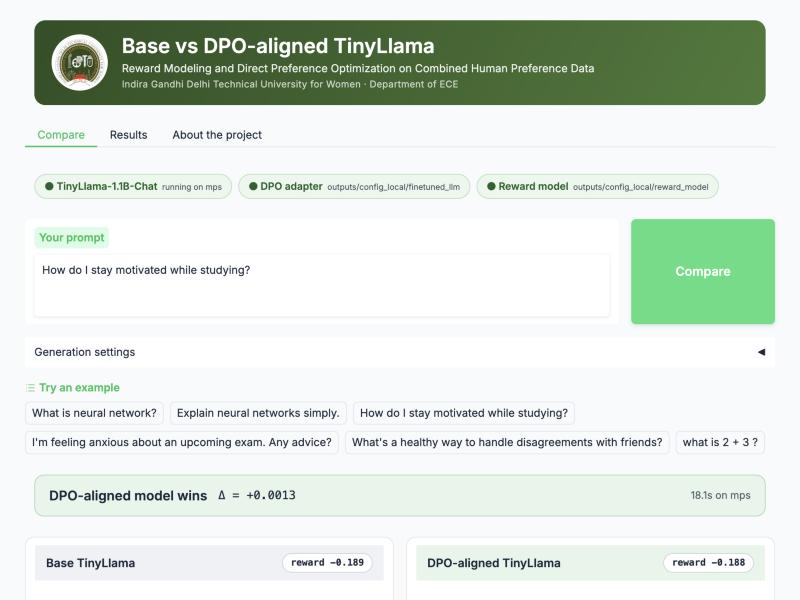
\includegraphics[width=0.92\textwidth]{figures/ui_compare_top.jpg}
\caption[Web application: Compare tab (input)]{Web application, Compare tab: model status, prompt box, example prompts and the result banner.}
\label{fig:ui-top}
\end{figure}

\begin{figure}[H]
\centering
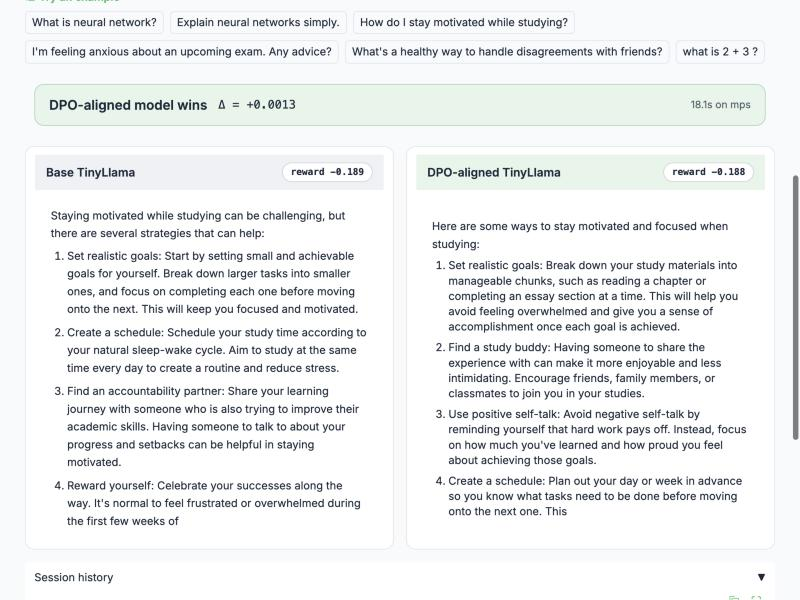
\includegraphics[width=0.92\textwidth]{figures/ui_compare_answers.jpg}
\caption[Web application: Compare tab (answers)]{Web application, Compare tab: base and DPO answers side by side with their reward scores.}
\label{fig:ui-answers}
\end{figure}

\begin{figure}[H]
\centering
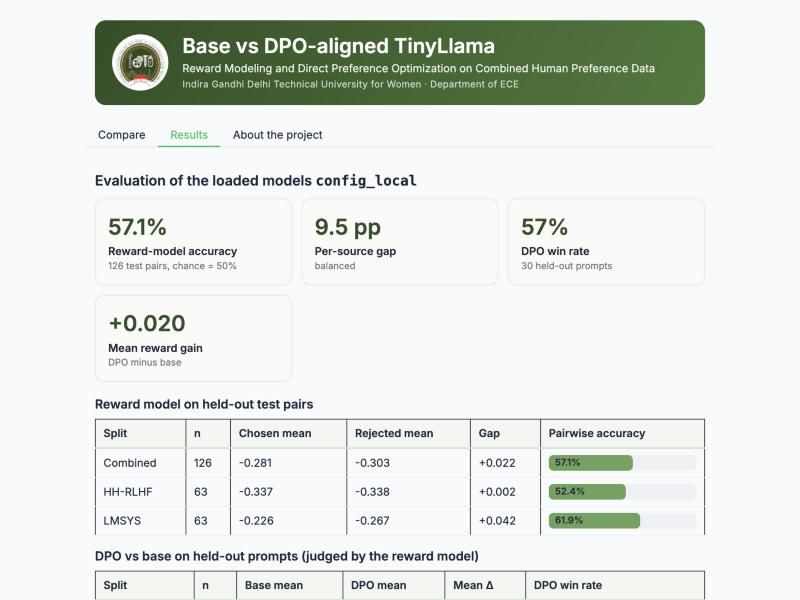
\includegraphics[width=0.92\textwidth]{figures/ui_results.jpg}
\caption[Web application: Results tab]{Web application, Results tab for the local configuration: summary tiles and per-source reward-model accuracy.}
\label{fig:ui-results}
\end{figure}

\begin{figure}[H]
\centering
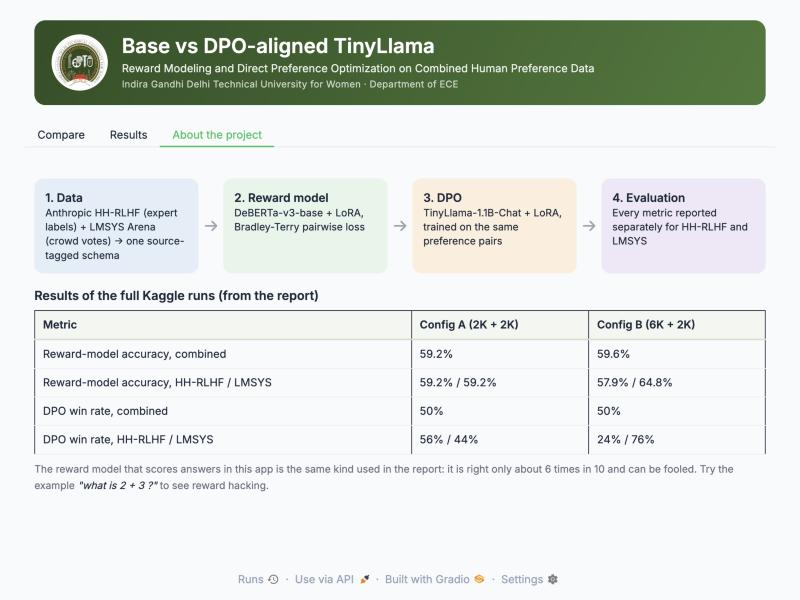
\includegraphics[width=0.92\textwidth]{figures/ui_about.jpg}
\caption[Web application: About tab]{Web application, About tab: pipeline overview and the results of the two Kaggle configurations.}
\label{fig:ui-about}
\end{figure}

\section{Engineering Challenges and Fixes}
\label{sec:impl-fixes}

Getting current versions of Transformers, TRL and PEFT to work on a T4, and later on an M1 laptop, threw up a series of problems, and several of them gave no error at all. Table~\ref{tab:fixes} lists them, and the most important ones are explained after the table.

{\footnotesize
\begin{longtable}{@{}L{0.5cm}L{4.0cm}L{4.3cm}L{5.0cm}@{}}
\caption[Implementation problems and fixes]{Problems encountered during implementation and their fixes.}\label{tab:fixes}\\
\toprule
\textbf{\#} & \textbf{Symptom} & \textbf{Root cause} & \textbf{Fix}\\
\midrule\endfirsthead
\toprule
\textbf{\#} & \textbf{Symptom} & \textbf{Root cause} & \textbf{Fix}\\
\midrule\endhead
\bottomrule\endfoot
1 & Reward scores are NaN; accuracy meaningless & DeBERTa-v3 disentangled attention overflows in FP16/BF16 & Load the RM in FP32 (fits easily at 184M parameters); NaN guards in scoring\\
2 & Crash in the FP16 gradient scaler: \texttt{NotImplementedError} \ldots\ \emph{not implemented for BFloat16} & TinyLlama's default BF16 layers + FP16 GradScaler; T4 lacks BF16 & FP16 compute for the 4-bit layers, FP16 for the remaining layers, mixed precision switched off in the trainers\\
3 & Reloaded RM gives different, unreliable scores from those seen in training & PEFT saved LoRA + classifier but \emph{not} the randomly initialised pooler; a fresh load re-randomises it & Add the pooler to \texttt{modules\_to\_save} so it is trained, saved and restored\\
4 & Old RM checkpoint fails to load after switching backbone & An adapter from the TinyLlama prototype was still in the working folder & First cell reads each \texttt{adapter\_config.json} and deletes checkpoints for the wrong backbone\\
5 & Device-mismatch errors on 2-GPU machine & Automatic placement put the model on \texttt{cuda:1} while inputs went to \texttt{cuda:0} & Send inputs to the device that holds the model's first parameter\\
6 & Validation and test sets overlapped & Same tail rows carved twice & Single-pass stratified split; disjoint slices\\
7 & Most LMSYS multi-turn rows disappeared & Over-length rows rejected rather than truncated & Truncate fields to 1,500 chars\\
8 & Cross-model context contamination & Earlier turns of A and B came from different models & Keep only the final user turn and final responses\\
9 & Attribute errors iterating LMSYS rows & Column names with trailing spaces; NaN values & Strip column names, check the schema, parse with \texttt{safe\_parse}\\
10 & Tokeniser crash on some LMSYS text & Unpaired UTF-16 surrogates & \texttt{clean\_text} removes them\\
11 & PEFT import error mentioning torchao & Kaggle ships torchao 0.10; PEFT needs $\ge$0.16 & Force-reinstall torchao and purge it from \texttt{sys.modules}\\
12 & TRL import crash & wandb/protobuf version mismatch & Upgrade wandb and disable it with environment variables\\
13 & Trained models lost between sessions & \texttt{/kaggle/working} is wiped & Save a notebook version and auto-detect adapters among the input datasets\\
14 & Gradient-checkpointing error with LoRA RM & Inputs did not require grad for non-quantised PEFT model & Call \texttt{enable\_input\_}\allowbreak\texttt{require\_grads()} on the model\\
15 & DPO over-fitting, later epochs degrade (config B) & High LR, too many epochs & LR $5\!\times\!10^{-5}\!\to\!10^{-5}$, $\beta$ 0.1$\to$0.15, best-checkpoint reload\\
16 & DPO stopped at step 3 on the 8\,GB M1 with an MPS ``Insufficient Memory'' error & FP16 TinyLlama plus two sequences per step exceeded unified memory & One pair per step with 8-step accumulation, 256-token DPO inputs, and the MPS memory cap lifted with an environment variable (Appendix~\ref{app:repro})\\
17 & LMSYS file not available outside Kaggle & Competition data needs a Kaggle login & Download the identical public copy (\texttt{lmarena-ai/}\allowbreak\texttt{arena-human-preference-55k}) from the HuggingFace Hub\\
\end{longtable}
}

\paragraph{The pooler problem (fix 3).} This was the hardest bug to find. In DeBERTa the classification head is a pooler followed by a classifier. Neither is part of the downloaded checkpoint (the loading report marks both \texttt{MISSING}), so both start with random values. With \texttt{TaskType.SEQ\_CLS}, PEFT trains and saves the classifier on its own, but the pooler, with 590,592 parameters, stayed frozen at its random start and was never saved. When a later cell loaded the reward model again, it received a \emph{new} random pooler, and the trained adapters and classifier were now attached to a layer they had never seen. As a result, scores at evaluation time did not match scores during training. Adding \texttt{modules\_to\_save=[\textquotedbl{}pooler\textquotedbl{}]} makes the pooler trainable, stores it with the adapter, and \texttt{PeftModel.from\_pretrained} puts it back exactly.

\paragraph{Number formats (fixes 1, 2 and 16).} Our two models need opposite settings. DeBERTa-v3 has to run in FP32 because its attention overflows in 16-bit. TinyLlama's 4-bit layers have to compute in FP16, because the T4 cannot do BF16 and mixing BF16 weights with an FP16 gradient scaler crashes. Turning off the trainers' mixed-precision options removes the gradient scaler completely, and memory is already saved by the 4-bit weights and LoRA. On the 8\,GB M1 laptop the policy cannot be quantised (bitsandbytes needs CUDA), so it runs in plain FP16, and DPO had to be cut to one pair per step with 256-token inputs to fit.

\section{Summary}
In this chapter we walked through the ten modules: the environment and saving logic, the two dataset parsers, the shared filter and per-source split, the DeBERTa-v3 reward model, 4-bit DPO training of TinyLlama, and the generation, evaluation and live-demo code. We then showed how this code became a reusable package and web application, listed the settings of every configuration, and recorded the problems we fixed. Some of them, such as the unsaved pooler, would have silently ruined the evaluation if they had not been caught. Chapter~\ref{ch:results} presents the results.

\chapter{Results and Discussion}
\label{ch:results}

This chapter gives our results. Sections~\ref{sec:setup}--\ref{sec:qual} contain the \textbf{measured results} of the two Kaggle runs, copied directly from the outputs of the notebooks we submit: configuration~A (\texttt{mini-6\_working}) and configuration~B (\texttt{mini-7-fixed}). Section~\ref{sec:local} adds the results of the smaller \emph{local} run made with the packaged system on a laptop. Section~\ref{sec:reported} then shows, separately, the \textbf{numbers given in our earlier IEEE-style paper draft}. Those numbers are higher than anything our code produced and we could not reproduce them, so every table and figure taken from the draft carries the label ``Reported in paper draft'' and the mark~\reportedtag. Section~\ref{sec:discussion} discusses all of these results together.

\section{Experimental Setup}
\label{sec:setup}

\subsection{Configurations}
We ran the whole pipeline twice on Kaggle's two T4 GPUs. Both runs use the code of Chapter~\ref{ch:impl}; they differ only in the data mix and the settings (Tables~\ref{tab:rm-hparams} and~\ref{tab:dpo-hparams}):
\begin{itemize}
  \item \textbf{Configuration A (balanced):} 2,000 pairs from each source. Reward model with LoRA rank 32, two epochs, learning rate $2\times10^{-5}$. DPO on 1,500 pairs with rank-16 LoRA on the attention layers only, learning rate $5\times10^{-5}$, $\beta$=0.1, two epochs.
  \item \textbf{Configuration B (more HH-RLHF):} 6,000 HH-RLHF and 2,000 LMSYS pairs. Reward model with LoRA rank 64, three epochs, learning rate $1\times10^{-5}$. DPO on 3,000 pairs (two HH-RLHF for every LMSYS pair) with rank-32 LoRA on attention and feed-forward layers, learning rate $1\times10^{-5}$, $\beta$=0.15, keeping the checkpoint with the best validation loss.
\end{itemize}

\subsection{Evaluation protocol}
\begin{enumerate}
  \item \textbf{RM evaluation:} pairwise accuracy and mean reward gap on the full held-out test split (250 pairs in A, 500 in B), overall and per source.
  \item \textbf{Demo reel:} five fixed prompts (two factual, one study-skills, two socio-emotional), one sample per model, scored by the RM.
  \item \textbf{Held-out evaluation:} 25 HH-RLHF and 25 LMSYS prompts sampled from the test split with seed 42; one sample per model per prompt; win rate and mean $\Delta$ overall and per source.
  \item \textbf{Interactive session (config.\ A):} seven prompts typed live during a demonstration.
\end{enumerate}

\subsection{Statistical resolution}
Our test sets are small, so it helps to know how much a percentage can move by chance alone. For $n$ yes/no outcomes near 50\%, a 95\% interval is roughly $\pm1.96\sqrt{0.25/n}$. That is about $\pm$13.9 points for 50 prompts and $\pm$19.6 points for 25. A difference in win rate smaller than this should not be read as a real effect. For the reward-model test sets the margins are about $\pm$6.1 points ($n$=250), $\pm$4.3 ($n$=500), $\pm$5.0 ($n$=375) and $\pm$8.6 ($n$=125).

\section{Dataset Analysis}
\label{sec:res-data}

Figures~\ref{fig:m6-dataset} and~\ref{fig:m7-dataset} describe the training data of the two configurations. Prompt lengths look similar for both sources, but LMSYS chosen answers are clearly longer than HH-RLHF ones, and their long tail is cut at 1,500 characters. Because the two sources differ this much in length, a reward model that learned ``longer is better'' from LMSYS might carry that rule over to HH-RLHF. Checking each source separately is how we would notice.

\begin{figure}[H]
\centering
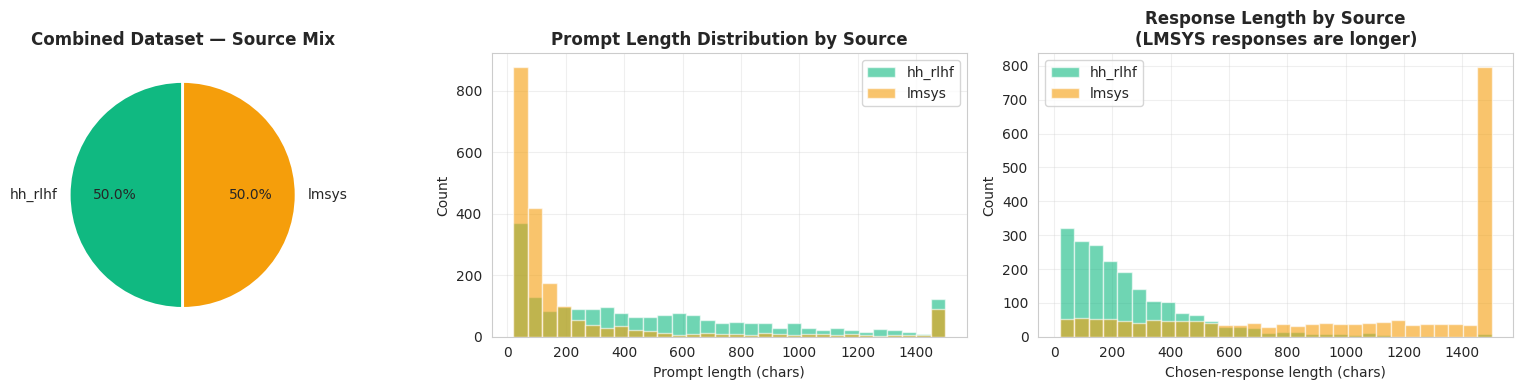
\includegraphics[width=\textwidth]{figures/m6_14_1.png}
\caption[Dataset composition, configuration A]{Configuration A dataset composition: (a) 50/50 source mix, (b) prompt length and (c) chosen-response length by source (measured, \texttt{mini-6}).}
\label{fig:m6-dataset}
\end{figure}

\begin{figure}[H]
\centering
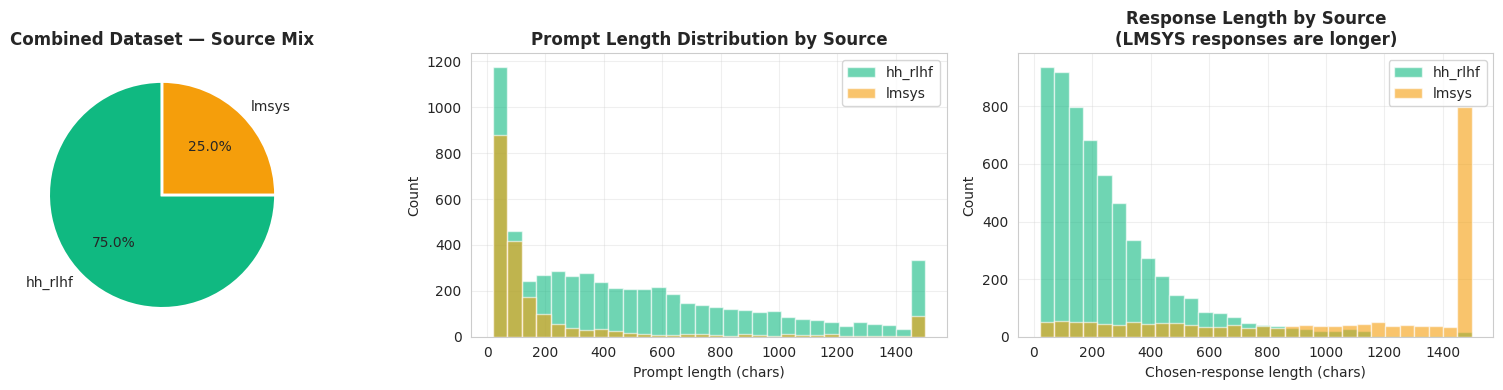
\includegraphics[width=\textwidth]{figures/m7_14_1.png}
\caption[Dataset composition, configuration B]{Configuration B dataset composition: 75/25 HH-RLHF/LMSYS mix (measured, \texttt{mini-7}).}
\label{fig:m7-dataset}
\end{figure}

\section{Reward Model Results}
\label{sec:res-rm}

\subsection{Training dynamics}
Figures~\ref{fig:m6-rmloss} and~\ref{fig:m7-rmloss} plot the reward model's training and validation loss. Both start at $\log 2\approx0.693$, which is what a model that cannot tell the two answers apart scores. In configuration A the validation loss reaches about 0.667 after roughly 210 steps (two epochs with 32 pairs per step). Configuration B, with twice the data and three epochs, reaches about 0.653 after roughly 650 steps, but stops improving after step 400 while the training loss keeps jumping up and down. Neither curve diverges. The improvement is small, though: a loss of 0.653 means the model gives the correct answer an average probability of only about $e^{-0.653}\approx0.52$. It is right more often than wrong, but not by much.

\begin{figure}[H]
\centering
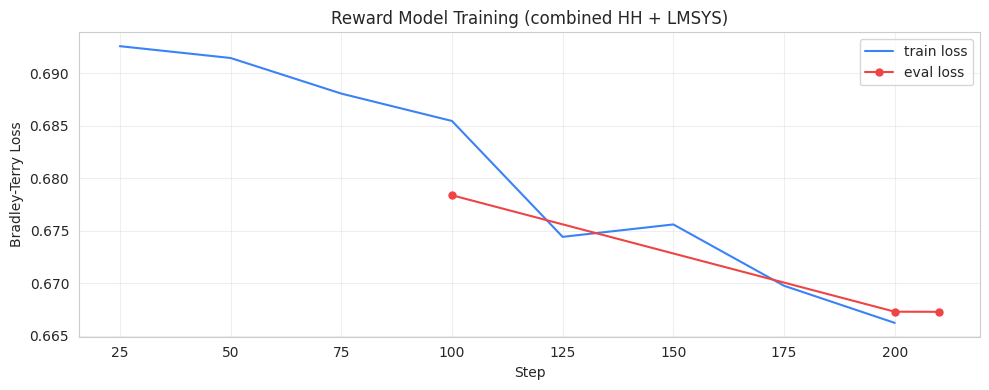
\includegraphics[width=0.85\textwidth]{figures/m6_25_3.png}
\caption[Reward-model loss, configuration A]{Reward-model training and validation loss, configuration A (measured).}
\label{fig:m6-rmloss}
\end{figure}

\begin{figure}[H]
\centering
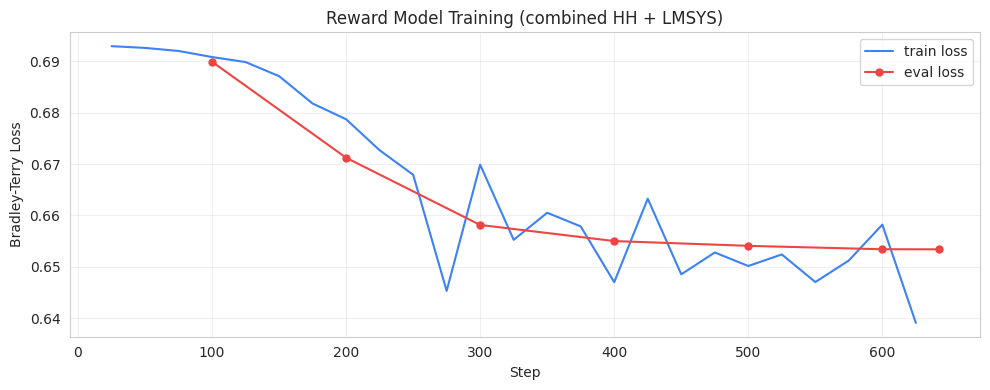
\includegraphics[width=0.85\textwidth]{figures/m7_25_3.png}
\caption[Reward-model loss, configuration B]{Reward-model training and validation loss, configuration B (measured).}
\label{fig:m7-rmloss}
\end{figure}

\subsection{Held-out test accuracy}
Table~\ref{tab:rm-results} gives the per-source test results of both configurations, as printed by the notebooks.

\begin{table}[!htbp]
\centering
\caption[Reward-model test results (A and B)]{Reward-model evaluation on the held-out test split (measured). The gap is the mean of chosen minus rejected reward.}
\label{tab:rm-results}
\small\setlength{\tabcolsep}{4.5pt}
\begin{tabular}{@{}llrrrrc@{}}
\toprule
\textbf{Config.} & \textbf{Split} & \textbf{$n$} & \textbf{Chosen $\bar r$} & \textbf{Rejected $\bar r$} & \textbf{Gap} & \textbf{Pairwise acc.}\\
\midrule
\multirow{3}{*}{A (2K+2K)} & Combined & 250 & $-0.4744$ & $-0.5432$ & $+0.0688$ & \textbf{59.2\%}\\
 & HH-RLHF & 125 & $-0.6847$ & $-0.7237$ & $+0.0390$ & 59.2\%\\
 & LMSYS & 125 & $-0.2642$ & $-0.3627$ & $+0.0985$ & 59.2\%\\
\midrule
\multirow{3}{*}{B (6K+2K)} & Combined & 500 & $-0.5502$ & $-0.6677$ & $+0.1175$ & \textbf{59.6\%}\\
 & HH-RLHF & 375 & $-0.6931$ & $-0.8124$ & $+0.1192$ & 57.9\%\\
 & LMSYS & 125 & $-0.1215$ & $-0.2337$ & $+0.1122$ & 64.8\%\\
\midrule
-- & Random baseline & -- & -- & -- & 0 & 50.0\%\\
\bottomrule
\end{tabular}
\end{table}

\paragraph{Better than guessing.} Both reward models beat the 50\% baseline by more than the margin of error; the 95\% intervals are about [53\%, 65\%] for A and [55\%, 64\%] for B. In every subset the average score of chosen answers is above that of rejected answers, which is the pass condition we set in the notebook.

\paragraph{Balance between sources.} In configuration A the reward model gets \emph{exactly} the same accuracy on both sources, 74 correct out of 125 each. In configuration B the gap is 6.9 points (57.9\% against 64.8\%). Both are inside our 10-point limit, so neither model has locked onto one source. The direction of B's gap surprised us: B saw three times more HH-RLHF pairs than LMSYS pairs, yet it does better on LMSYS. Our explanation is that an LMSYS pair often compares answers from two quite different chatbots, which is easier to judge, whereas the two answers in an HH-RLHF pair come from very similar Anthropic models and are often nearly the same.

\paragraph{More data did not help much.} Going from A to B, with three times the HH-RLHF data and one more epoch, made the model more confident (average gap 0.069 to 0.118) but hardly more accurate (59.2\% to 59.6\%). At this scale, a 184M-parameter encoder on a few thousand noisy pairs seems limited by its size and by the label noise rather than by the amount of data.

\subsection{Score distributions}
Figures~\ref{fig:m6-rmdist} and~\ref{fig:m7-rmdist} show how the scores and the per-pair gaps are spread. The chosen and rejected histograms overlap a lot, and the gap histograms sit only slightly to the right of zero, which fits a weak but real signal. In configuration A a large group of LMSYS scores bunches up near the top of the range (about $+0.1$), as if the classifier output saturates for some inputs.

\begin{figure}[H]
\centering
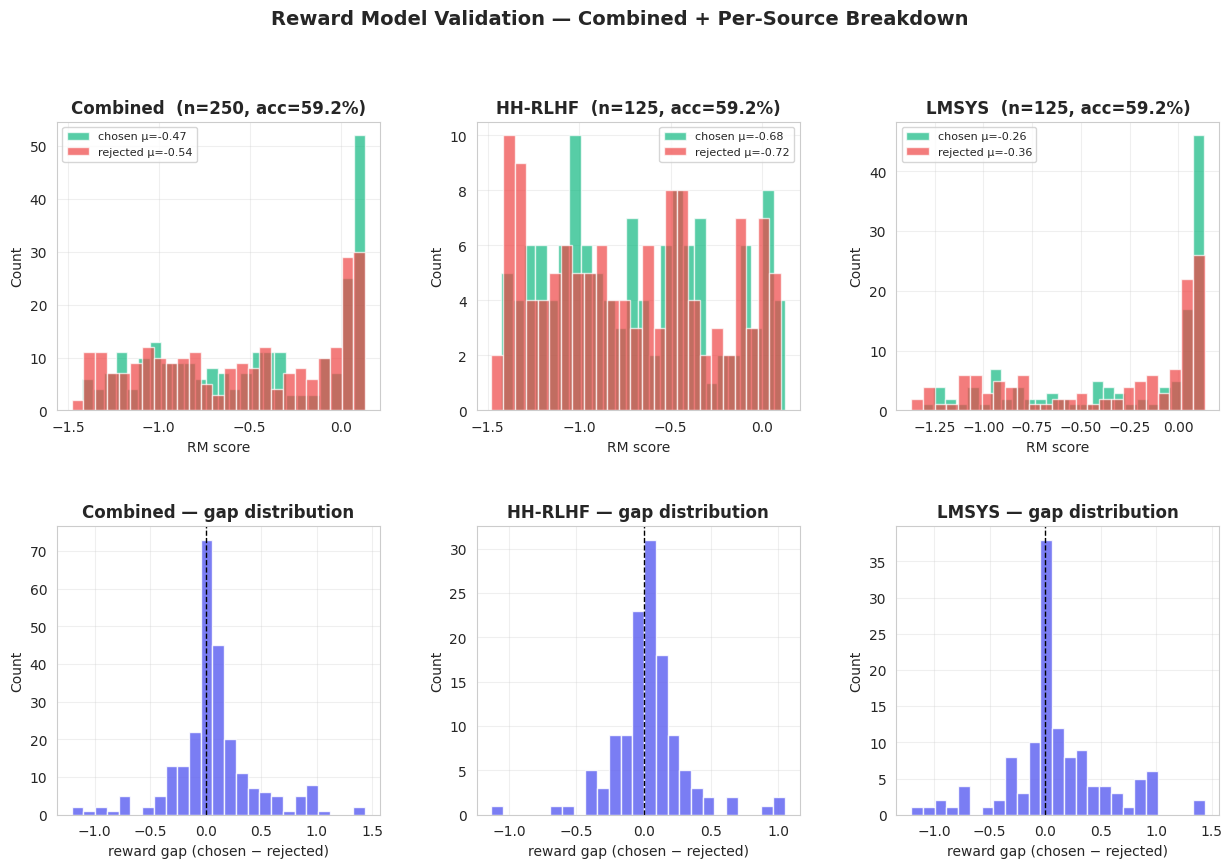
\includegraphics[width=\textwidth]{figures/m6_24_2.png}
\caption[Reward-model score distributions, configuration A]{Configuration A reward-model validation: score histograms (top) and gap distributions (bottom) for the combined, HH-RLHF and LMSYS test subsets (measured).}
\label{fig:m6-rmdist}
\end{figure}

\begin{figure}[H]
\centering
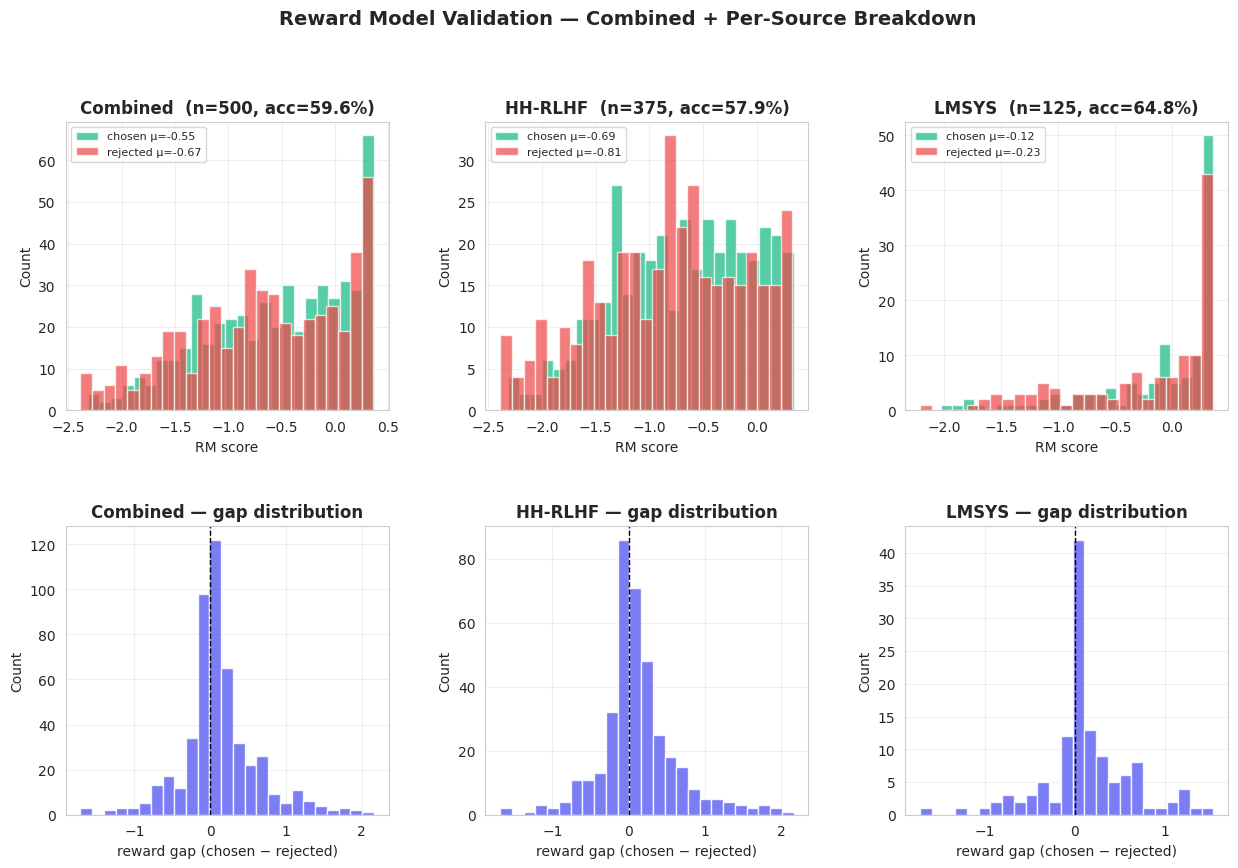
\includegraphics[width=\textwidth]{figures/m7_24_2.png}
\caption[Reward-model score distributions, configuration B]{Configuration B reward-model validation: score histograms and gap distributions per subset (measured).}
\label{fig:m7-rmdist}
\end{figure}

\section{DPO Training Results}
\label{sec:res-dpo-train}

Figures~\ref{fig:m6-dpocurves} and~\ref{fig:m7-dpocurves} show the DPO training diagnostics logged by TRL: loss, mean implicit rewards of chosen and rejected responses, and implicit-reward accuracy.

\begin{figure}[H]
\centering
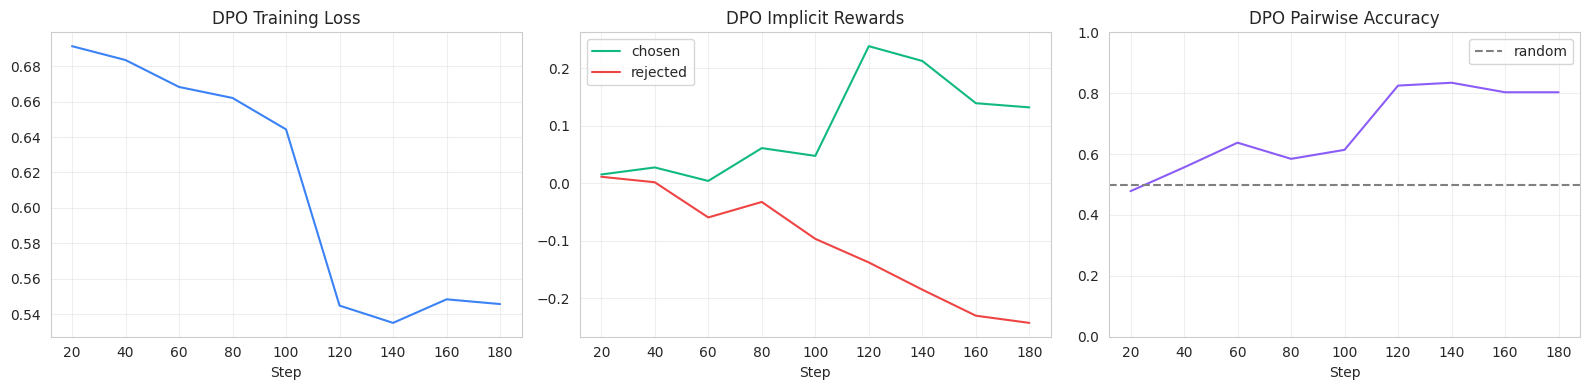
\includegraphics[width=\textwidth]{figures/m6_32_4.png}
\caption[DPO training curves, configuration A]{DPO training curves, configuration A: loss, implicit rewards and implicit-reward accuracy (measured).}
\label{fig:m6-dpocurves}
\end{figure}

\begin{figure}[H]
\centering
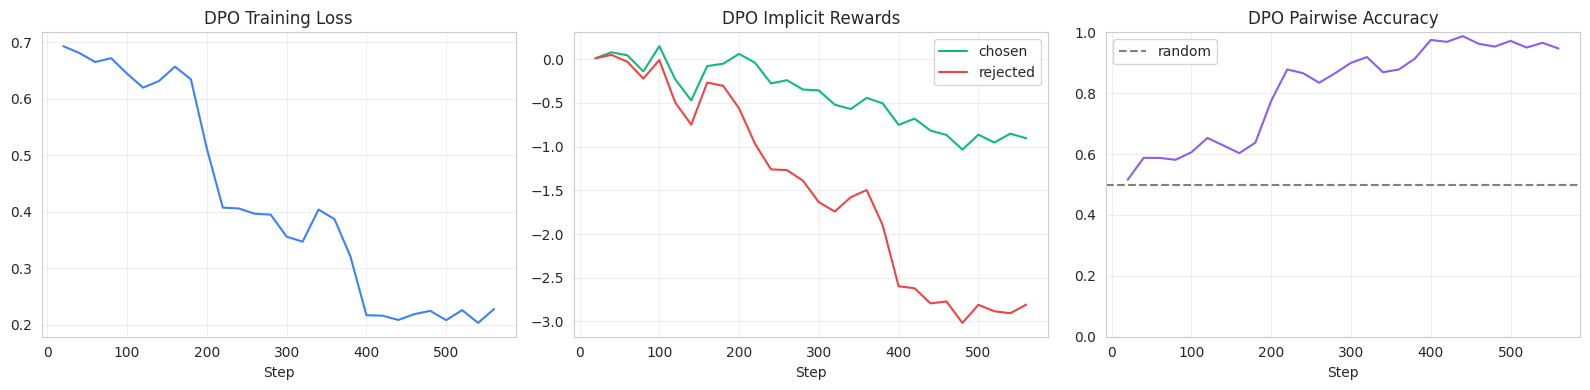
\includegraphics[width=\textwidth]{figures/m7_32_4.png}
\caption[DPO training curves, configuration B]{DPO training curves, configuration B (measured).}
\label{fig:m7-dpocurves}
\end{figure}

In configuration A the loss drops from 0.69 to about 0.54 in roughly 190 steps. The implicit reward of chosen answers climbs to about $+0.13$ and that of rejected answers falls to about $-0.24$, so the two move apart as intended, and the share of pairs ranked correctly rises from chance to about 80\%. Configuration B trains for about 560 steps and goes much further: the loss falls to about 0.2 and accuracy reaches about 95\% (Table~\ref{tab:dpo-log}). In B, however, \emph{both} implicit rewards turn negative, the chosen one to about $-0.9$ and the rejected one to about $-2.9$. The model is making both answers less likely, the rejected one much more so. This pattern is known from the DPO literature~\cite{azar2024ipo}. It suggests the model is memorising the particular training pairs rather than becoming more likely to write answers like the chosen ones.

\begin{table}[!htbp]
\centering
\caption[Final DPO log entries, configuration B]{Last five DPO log entries of configuration B (measured, as printed by the notebook).}
\label{tab:dpo-log}
\small
\begin{tabular}{@{}rrrrrrr@{}}
\toprule
\textbf{Step} & \textbf{Epoch} & \textbf{Loss} & \textbf{Chosen $\hat r$} & \textbf{Rejected $\hat r$} & \textbf{Margin} & \textbf{Accuracy}\\
\midrule
480 & 2.55 & 0.2242 & $-1.034$ & $-3.017$ & 1.983 & 95.3\%\\
500 & 2.66 & 0.2078 & $-0.863$ & $-2.810$ & 1.948 & 97.2\%\\
520 & 2.77 & 0.2255 & $-0.953$ & $-2.884$ & 1.932 & 95.0\%\\
540 & 2.87 & 0.2029 & $-0.851$ & $-2.907$ & 2.055 & 96.6\%\\
560 & 2.98 & 0.2274 & $-0.905$ & $-2.807$ & 1.903 & 94.7\%\\
\bottomrule
\end{tabular}
\end{table}

Measured by its own training objective, then, DPO worked in both runs. What matters more is whether the aligned model's answers are actually preferred, first by the reward model and ideally by people. That is the subject of the next sections.

\section{Base vs.\ DPO Comparison}
\label{sec:res-compare}

\subsection{Five-prompt demo reel}
Table~\ref{tab:demo} lists the reward scores of the base and DPO responses on the fixed demo prompts for both configurations.

\begin{table}[!htbp]
\centering
\caption[Five-prompt demo results]{Five-prompt demo reel: reward-model scores of base and DPO responses (measured).}
\label{tab:demo}
\footnotesize\setlength{\tabcolsep}{4pt}
\begin{tabularx}{\textwidth}{@{}>{\raggedright\arraybackslash}Xrrrcrrrc@{}}
\toprule
 & \multicolumn{4}{c}{\textbf{Configuration A}} & \multicolumn{4}{c}{\textbf{Configuration B}}\\
\cmidrule(lr){2-5}\cmidrule(l){6-9}
\textbf{Prompt} & \textbf{Base} & \textbf{DPO} & \textbf{$\Delta$} & \textbf{Win} & \textbf{Base} & \textbf{DPO} & \textbf{$\Delta$} & \textbf{Win}\\
\midrule
What is neural network? & $-0.658$ & $-0.156$ & $+0.502$ & DPO & $+0.124$ & $+0.122$ & $-0.001$ & Base\\
Explain neural networks simply. & $-0.203$ & $-0.158$ & $+0.045$ & DPO & $+0.093$ & $+0.122$ & $+0.030$ & DPO\\
How do I stay motivated while studying? & $-0.315$ & $-0.141$ & $+0.173$ & DPO & $+0.140$ & $+0.109$ & $-0.031$ & Base\\
Anxious about an upcoming exam. Any advice? & $-0.143$ & $-0.196$ & $-0.053$ & Base & $+0.056$ & $+0.031$ & $-0.025$ & Base\\
Healthy way to handle disagreements with friends? & $-0.106$ & $-0.155$ & $-0.049$ & Base & $+0.054$ & $+0.068$ & $+0.014$ & DPO\\
\midrule
\textbf{Mean / wins} & $-0.285$ & $-0.161$ & $\mathbf{+0.124}$ & \textbf{3/5} & $+0.093$ & $+0.091$ & $\mathbf{-0.003}$ & \textbf{2/5}\\
\bottomrule
\end{tabularx}
\end{table}

\begin{figure}[H]
\centering
\begin{subfigure}{0.85\textwidth}\centering
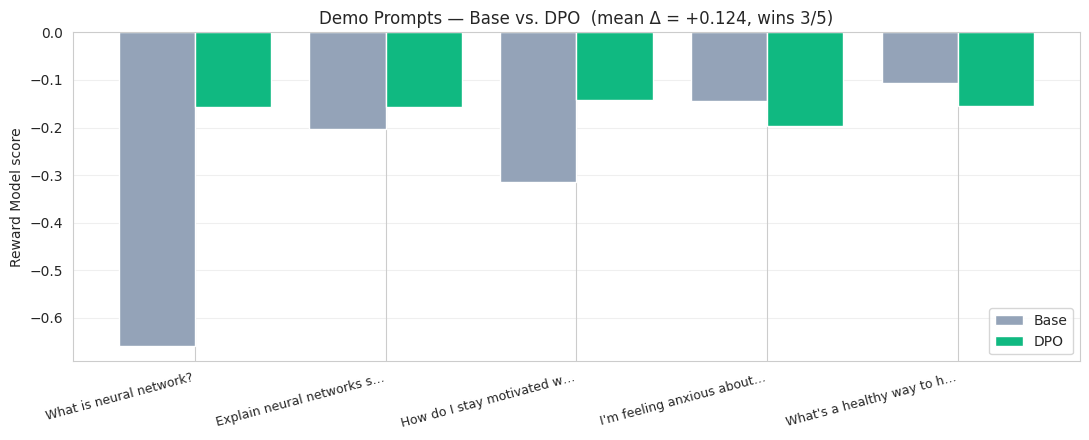
\includegraphics[width=\textwidth]{figures/m6_42_5.png}
\caption{Configuration A}
\end{subfigure}\\[6pt]
\begin{subfigure}{0.85\textwidth}\centering
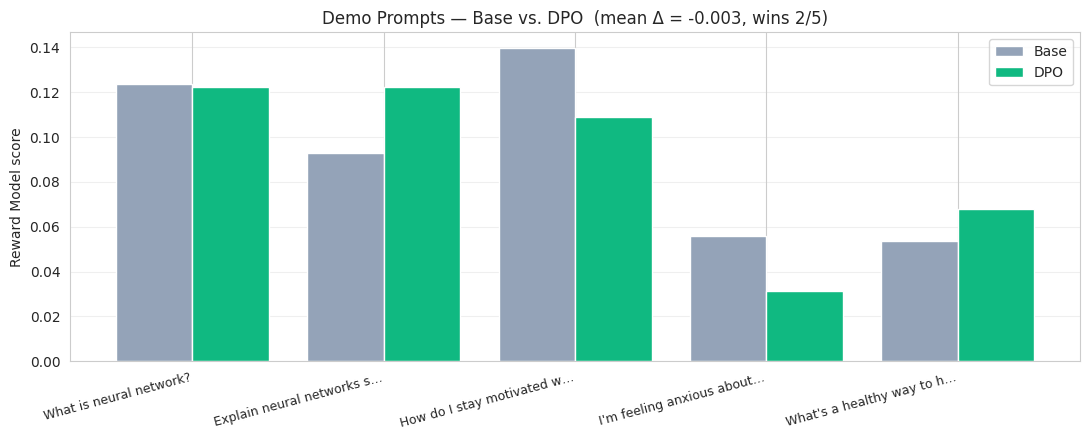
\includegraphics[width=\textwidth]{figures/m7_42_5.png}
\caption{Configuration B}
\end{subfigure}
\caption[Demo-reel scores, base vs.\ DPO]{Demo-reel reward scores, base vs.\ DPO (measured).}
\label{fig:demo}
\end{figure}

In configuration A the DPO model wins three of the five prompts and improves the average score by $+0.124$, mostly because of one large gain on the first factual question. The base model wins the two prompts about emotions by small margins. In configuration B the differences are about ten times smaller ($|\Delta|\le0.031$) and the average change is close to zero. One sample each on five prompts cannot support any conclusion; we include the demo set to illustrate the outputs, not to measure them.

\subsection{Held-out evaluation on 50 prompts}
Table~\ref{tab:heldout} gives the main quantitative result for the aligned policy, and Figures~\ref{fig:m6-headline} and~\ref{fig:m7-headline} visualise it.

\begin{table}[!htbp]
\centering
\caption[Held-out win rates (A and B)]{Held-out evaluation, DPO vs.\ base on 25 + 25 test prompts judged by the reward model (measured).}
\label{tab:heldout}
\small
\begin{tabular}{@{}llrrrrc@{}}
\toprule
\textbf{Config.} & \textbf{Split} & \textbf{$n$} & \textbf{Base $\bar r$} & \textbf{DPO $\bar r$} & \textbf{Mean $\Delta$} & \textbf{Win rate}\\
\midrule
\multirow{3}{*}{A} & Combined & 50 & $-0.2910$ & $-0.2639$ & $+0.0270$ & \textbf{50.0\%}\\
 & HH-RLHF & 25 & $-0.3250$ & $-0.2821$ & $+0.0429$ & 56.0\%\\
 & LMSYS & 25 & $-0.2569$ & $-0.2458$ & $+0.0111$ & 44.0\%\\
\midrule
\multirow{3}{*}{B} & Combined & 50 & $-0.1210$ & $-0.1442$ & $-0.0232$ & \textbf{50.0\%}\\
 & HH-RLHF & 25 & $-0.1221$ & $-0.2832$ & $-0.1611$ & 24.0\%\\
 & LMSYS & 25 & $-0.1200$ & $-0.0052$ & $+0.1148$ & 76.0\%\\
\midrule
-- & Random baseline & -- & -- & -- & 0 & 50.0\%\\
\bottomrule
\end{tabular}
\end{table}

\begin{figure}[H]
\centering
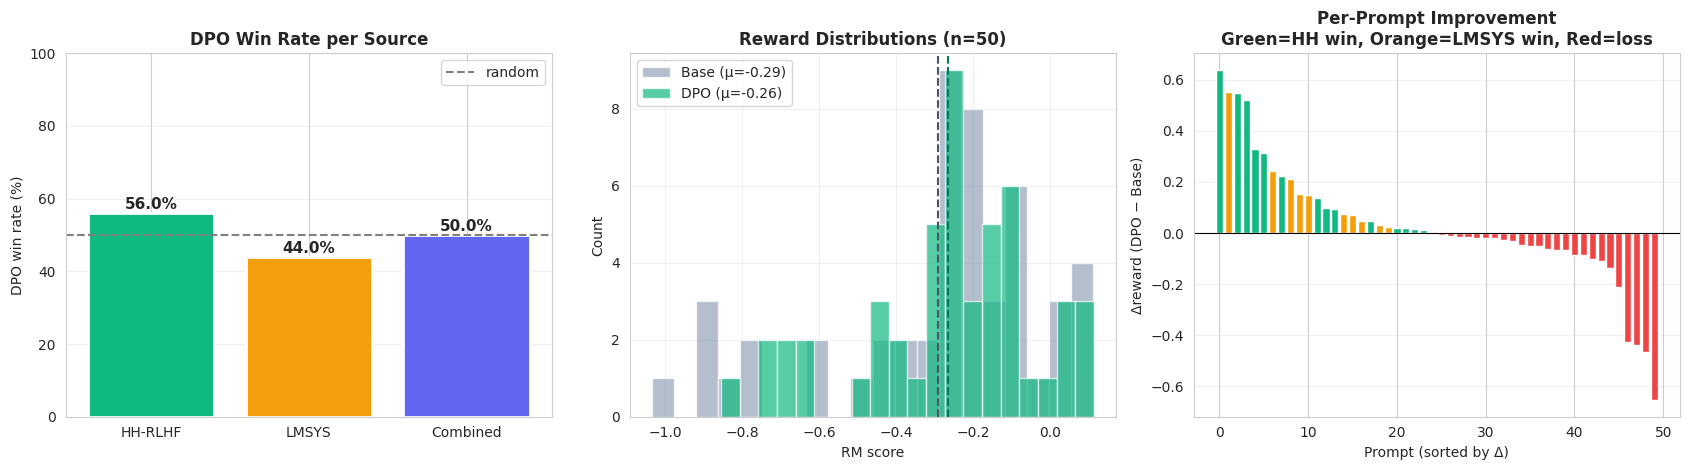
\includegraphics[width=\textwidth]{figures/m6_45_6.png}
\caption[Held-out evaluation, configuration A]{Configuration A held-out evaluation: (a) win rate per source, (b) reward distributions of base and DPO responses, (c) per-prompt $\Delta$ sorted, coloured by source (measured).}
\label{fig:m6-headline}
\end{figure}

\begin{figure}[H]
\centering
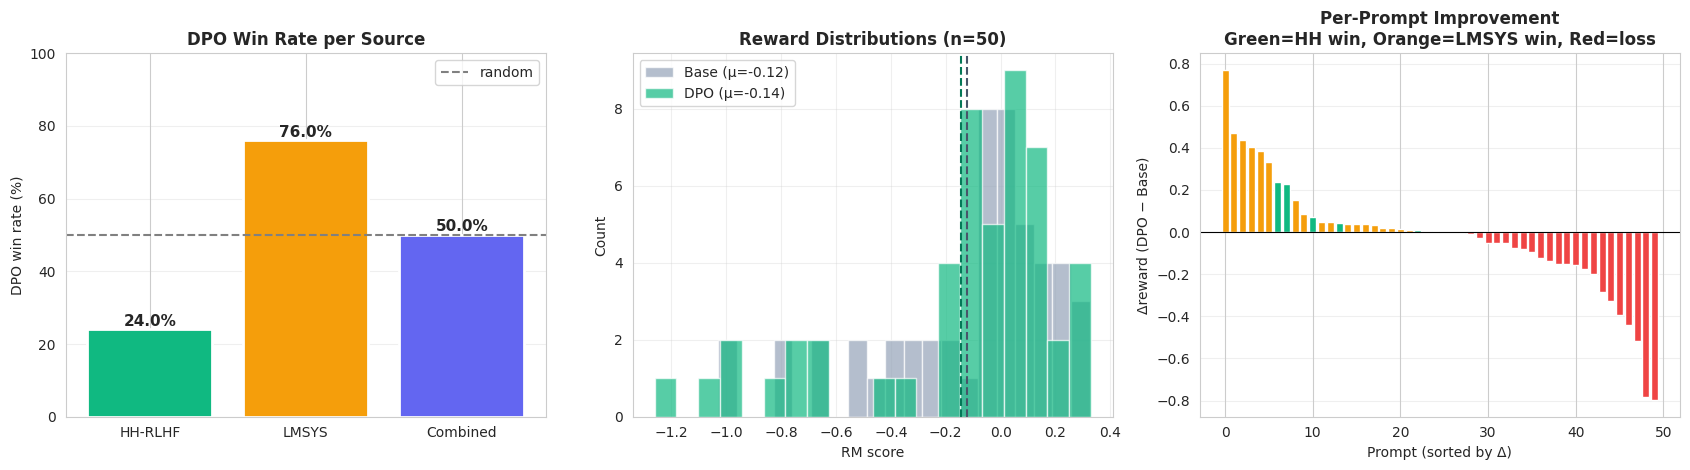
\includegraphics[width=\textwidth]{figures/m7_45_6.png}
\caption[Held-out evaluation, configuration B]{Configuration B held-out evaluation (measured). The per-source panel shows a strong split: DPO loses on most HH-RLHF prompts and wins on most LMSYS prompts.}
\label{fig:m7-headline}
\end{figure}

\paragraph{Configuration A.} DPO wins exactly half of the 50 prompts, and the average score rises by only $+0.027$. The per-source figures, 56\% and 44\%, are well within the $\pm$19.6-point margin for 25 prompts, so they are not different from chance. In the sorted chart the biggest gains are on HH-RLHF prompts, but there are about as many losses.

\paragraph{Configuration B.} Again DPO wins exactly half overall, but this time the two sources go in opposite directions, and strongly: 76\% wins on LMSYS prompts (19 of 25) and only 24\% on HH-RLHF prompts (6 of 25). A two-sided binomial test against 50\% gives $p\approx0.015$ for each source. The average score rises by $+0.115$ on LMSYS and falls by $0.161$ on HH-RLHF. Looking only at the overall figure, we would have concluded that DPO did nothing. Split by source, it is clear that the more heavily trained model has changed in a way the reward model likes for open Arena-style questions and dislikes for HH-style dialogue replies.

\subsection{Interactive session (configuration A)}
Table~\ref{tab:interactive} lists the seven prompts typed during a live demonstration of configuration A. DPO won four of them, with an average change of $+0.172$, but its biggest win turns out to be a problem, as Section~\ref{sec:hacking} shows.

\begin{table}[!htbp]
\centering
\caption[Interactive session prompts]{Interactive demonstration prompts, configuration A (measured).}
\label{tab:interactive}
\small
\begin{tabularx}{\textwidth}{@{}Yrrrc@{}}
\toprule
\textbf{Prompt (as typed)} & \textbf{Base} & \textbf{DPO} & \textbf{$\Delta$} & \textbf{Winner}\\
\midrule
what is ml & $-0.5099$ & $-0.2154$ & $+0.2944$ & DPO\\
what is the use of caffeine? & $-0.2088$ & $-0.2850$ & $-0.0763$ & Base\\
what is machine learning & $-0.2181$ & $-0.4195$ & $-0.2014$ & Base\\
what is difference between ai and ml? & $-0.1348$ & $-0.1567$ & $-0.0219$ & Base\\
what is 2 + 3 ? & $-0.8746$ & $-0.1879$ & $+0.6867$ & DPO\\
what is neural network? & $-0.6804$ & $-0.2056$ & $+0.4748$ & DPO\\
What's a healthy way to handle disagreements with friends? & $-0.1656$ & $-0.1211$ & $+0.0446$ & DPO\\
\midrule
\textbf{Mean / wins} & & & $\mathbf{+0.1716}$ & \textbf{4/7}\\
\bottomrule
\end{tabularx}
\end{table}

\section{Qualitative Analysis}
\label{sec:qual}

\subsection{A genuine improvement}
Take the prompt \emph{``How do I stay motivated while studying?''} (configuration A, $\Delta=+0.173$). Both models answer with a numbered list. The base model's third tip says that if studying feels boring you should ``try finding something else that you enjoy doing'', such as watching TV, which defeats the purpose. The DPO answer is more practical: it turns a vague aim into a daily commitment (``I will work on my essays and assignments for 2 hours per day''), suggests finding people who can support you, and recommends tracking progress in a planner. Here we agree with the reward model that the DPO answer is more useful.

\subsection{A case of reward hacking}
\label{sec:hacking}
Now take \emph{``what is 2 + 3 ?''} (Table~\ref{tab:interactive}). The base model gets it right in an odd way, by writing a short Java program that prints 5. The DPO model starts well (``the sum of 2 and 3 will be 5'') but then wanders into rewording unrelated everyday sentences and claims that ``\texttt{2+3} is the same as \texttt{3 + 6}'', which is wrong. The reward model still rates the DPO answer $0.69$ higher, the largest gain in any of our evaluations.

This is reward hacking of exactly the kind described by Gao \emph{et al.}~\cite{gao2023overoptimization} and Casper \emph{et al.}~\cite{casper2023open}. Our small reward model has picked up surface signs of answers people liked, such as a friendly explaining tone, list-like structure and mathematical words, but it never checks whether an answer is correct. A model trained towards its preferences inherits those blind spots, and the same model used as a judge cannot catch them. For this reason we treat every win rate in this chapter as a rough indication, not as proof.

\section{Results of the Local System Run}
\label{sec:local}

After packaging the code (Section~\ref{sec:system}) we trained the \emph{local} configuration from scratch on an Apple M1 laptop with 8\,GB of memory, to check that the whole system works outside Kaggle. All numbers in this section come from that run's log files and its \texttt{metrics.json}.

\subsection{Training}
The reward model trained for 94 steps in 58 minutes. On the 124 validation pairs its loss fell from $0.693$ to $0.679$ and it ranked 65.2\% of pairs correctly. The first DPO attempt stopped at step 3 because the GPU ran out of memory. After we reduced DPO to one pair per step with 256-token inputs (Section~\ref{sec:impl-fixes}, fix 16), it completed 43 steps in 22 minutes. Its validation loss moved only from $0.693$ to $0.684$, and its implicit-reward accuracy on validation pairs was 56.4\%. This is a much weaker update than configuration A, which is expected from one epoch on 400 pairs.

\subsection{Evaluation}
\begin{table}[!htbp]
\centering
\caption[Local run: reward-model test results]{Local run: reward model on the 126 held-out test pairs (measured).}
\label{tab:local-rm}
\small
\begin{tabular}{@{}lrrrrc@{}}
\toprule
\textbf{Split} & \textbf{$n$} & \textbf{Chosen $\bar r$} & \textbf{Rejected $\bar r$} & \textbf{Gap} & \textbf{Pairwise acc.}\\
\midrule
Combined & 126 & $-0.281$ & $-0.303$ & $+0.022$ & \textbf{57.1\%}\\
HH-RLHF & 63 & $-0.337$ & $-0.338$ & $+0.002$ & 52.4\%\\
LMSYS & 63 & $-0.226$ & $-0.267$ & $+0.042$ & 61.9\%\\
\bottomrule
\end{tabular}
\end{table}

\begin{table}[!htbp]
\centering
\caption[Local run: DPO vs.\ base win rates]{Local run: DPO against base on 15 + 15 held-out prompts, judged by the local reward model (measured).}
\label{tab:local-dpo}
\small
\begin{tabular}{@{}lrrrrc@{}}
\toprule
\textbf{Split} & \textbf{$n$} & \textbf{Base $\bar r$} & \textbf{DPO $\bar r$} & \textbf{Mean $\Delta$} & \textbf{Win rate}\\
\midrule
Combined & 30 & $-0.257$ & $-0.237$ & $+0.020$ & 56.7\% (17/30)\\
HH-RLHF & 15 & $-0.232$ & $-0.225$ & $+0.007$ & 60.0\% (9/15)\\
LMSYS & 15 & $-0.283$ & $-0.249$ & $+0.033$ & 53.3\% (8/15)\\
\bottomrule
\end{tabular}
\end{table}

On the five demo prompts the DPO model won two (``Explain neural networks simply'', $\Delta=+0.198$, and the exam-anxiety prompt, $\Delta=+0.009$) and lost three by small margins, with a mean change of $+0.029$.

\subsection{What the local run shows}
With half the data and one epoch, the local reward model is slightly weaker than the Kaggle ones (57.1\% against about 59\%). It is again better on LMSYS than on HH-RLHF, the same direction as configuration B, and the 9.5-point gap is just inside our 10-point limit. The DPO model wins 17 of 30 prompts. With only 15 prompts per source the margin of error is about $\pm$25 points, so none of these win rates differs from chance. The value of this run is not its scores. It shows that the complete system, from raw data to a trained reward model, a trained policy, a per-source evaluation and a working web application, can be reproduced on a student laptop in about one and a half hours. Figure~\ref{fig:ui-results} shows these results as they appear in the application.

\section{Results Reported in the Earlier Paper Draft}
\label{sec:reported}

Earlier in the project we wrote an IEEE-format paper draft with the same title as this report. It gave much higher numbers than the ones measured above. We include them here so that the record is complete, but \textbf{kept apart from the measured results}. Neither of the submitted notebooks produced these numbers or figures, and we could not reproduce them, so they should be treated as unverified.

\begin{table}[!htbp]
\centering
\caption[Paper draft (not reproduced): reward-model results]{\reportedtag\ Reported in paper draft (not reproduced): reward-model test-set evaluation.}
\label{tab:rep-rm}
\small
\begin{tabular}{@{}lrrrrc@{}}
\toprule
\textbf{Split} & \textbf{$n$} & \textbf{Chosen $\bar r$} & \textbf{Rejected $\bar r$} & \textbf{Gap} & \textbf{Pairwise acc.}\\
\midrule
Combined & 250 & $+0.31$ & $-0.28$ & $+0.59$ & 72.6\%\\
HH-RLHF only & 125 & $+0.35$ & $-0.30$ & $+0.65$ & 74.1\%\\
LMSYS only & 125 & $+0.27$ & $-0.25$ & $+0.52$ & 71.0\%\\
Random baseline & -- & -- & -- & -- & 50.0\%\\
\bottomrule
\end{tabular}
\end{table}

\begin{table}[!htbp]
\centering
\caption[Paper draft (not reproduced): DPO win rates]{\reportedtag\ Reported in paper draft (not reproduced): DPO evaluation on 50 held-out prompts.}
\label{tab:rep-dpo}
\small
\begin{tabular}{@{}lrrrrc@{}}
\toprule
\textbf{Split} & \textbf{$n$} & \textbf{Base $\bar r$} & \textbf{DPO $\bar r$} & \textbf{$\Delta$} & \textbf{Win rate}\\
\midrule
Combined & 50 & $-0.12$ & $+0.25$ & $+0.37$ & 66.0\%\\
HH-RLHF prompts & 25 & $-0.10$ & $+0.28$ & $+0.38$ & 68.0\%\\
LMSYS prompts & 25 & $-0.14$ & $+0.22$ & $+0.36$ & 64.0\%\\
\bottomrule
\end{tabular}
\end{table}

\begin{table}[!htbp]
\centering
\caption[Paper draft (not reproduced): demo results]{\reportedtag\ Reported in paper draft (not reproduced): five-prompt demo reel. Note that the prompt set differs slightly from the one in the submitted notebooks (Table~\ref{tab:demo}).}
\label{tab:rep-demo}
\small
\begin{tabular}{@{}lrrrc@{}}
\toprule
\textbf{Prompt (truncated)} & \textbf{Base} & \textbf{DPO} & \textbf{$\Delta$} & \textbf{Winner}\\
\midrule
``What is machine learning?'' & $-0.18$ & $+0.31$ & $+0.49$ & DPO\\
``Explain neural networks simply.'' & $-0.05$ & $+0.28$ & $+0.33$ & DPO\\
``How do I stay motivated while studying?'' & $+0.12$ & $+0.44$ & $+0.32$ & DPO\\
``Feeling anxious about an upcoming exam.'' & $-0.22$ & $+0.35$ & $+0.57$ & DPO\\
``Handle disagreements with friends?'' & $+0.08$ & $+0.39$ & $+0.31$ & DPO\\
\midrule
Mean & $-0.05$ & $+0.35$ & $+0.40$ & 5/5\\
\bottomrule
\end{tabular}
\end{table}

\begin{table}[!htbp]
\centering
\caption[Paper draft (not reproduced): mixing ablation]{\reportedtag\ Reported in paper draft (not reproduced): ablation on dataset mixing.}
\label{tab:rep-ablation}
\small
\begin{tabular}{@{}lccc@{}}
\toprule
\textbf{RM training data} & \textbf{HH-RLHF acc.} & \textbf{LMSYS acc.} & \textbf{Combined}\\
\midrule
HH-RLHF only (2,000) & 75.2\% & 61.3\% & 68.3\%\\
LMSYS only (2,000) & 63.4\% & 72.8\% & 68.1\%\\
Combined (1K + 1K) & 73.8\% & 70.4\% & 72.1\%\\
Combined (2K + 2K) & 74.1\% & 71.0\% & 72.6\%\\
\bottomrule
\end{tabular}
\end{table}

\begin{table}[!htbp]
\centering
\caption[Paper draft: compute cost per stage]{\reportedtag\ Reported in paper draft: approximate wall-clock cost per stage on Kaggle T4$\times$2.}
\label{tab:rep-compute}
\small
\begin{tabular}{@{}llll@{}}
\toprule
\textbf{Stage} & \textbf{Examples} & \textbf{Epochs} & \textbf{Wall time}\\
\midrule
Dataset preprocessing & 4,000 & -- & $\sim$8 min\\
RM training & 3,500 (train) & 3 & $\sim$90 min\\
RM evaluation & 250 & -- & $\sim$5 min\\
DPO fine-tuning & 1,500 & 2 & $\sim$50 min\\
DPO evaluation & 50 prompts & -- & $\sim$15 min\\
Total (first run) & -- & -- & $\sim$2.5--3 h\\
Cached runs & -- & -- & $<$30 s\\
\bottomrule
\end{tabular}
\end{table}

The draft's figures follow (Figures~\ref{fig:rep-dataset}--\ref{fig:rep-dpoeval}). Two details stand out. Its reward-model accuracy curve (Figure~\ref{fig:rep-rmtrain}b) climbs to about 72\%, and its loss curve starts above 1.0. A Bradley--Terry loss on balanced pairs has to start at $\log 2\approx0.69$, as our measured curves in Figures~\ref{fig:m6-rmloss} and~\ref{fig:m7-rmloss} do.

\begin{figure}[H]
\centering
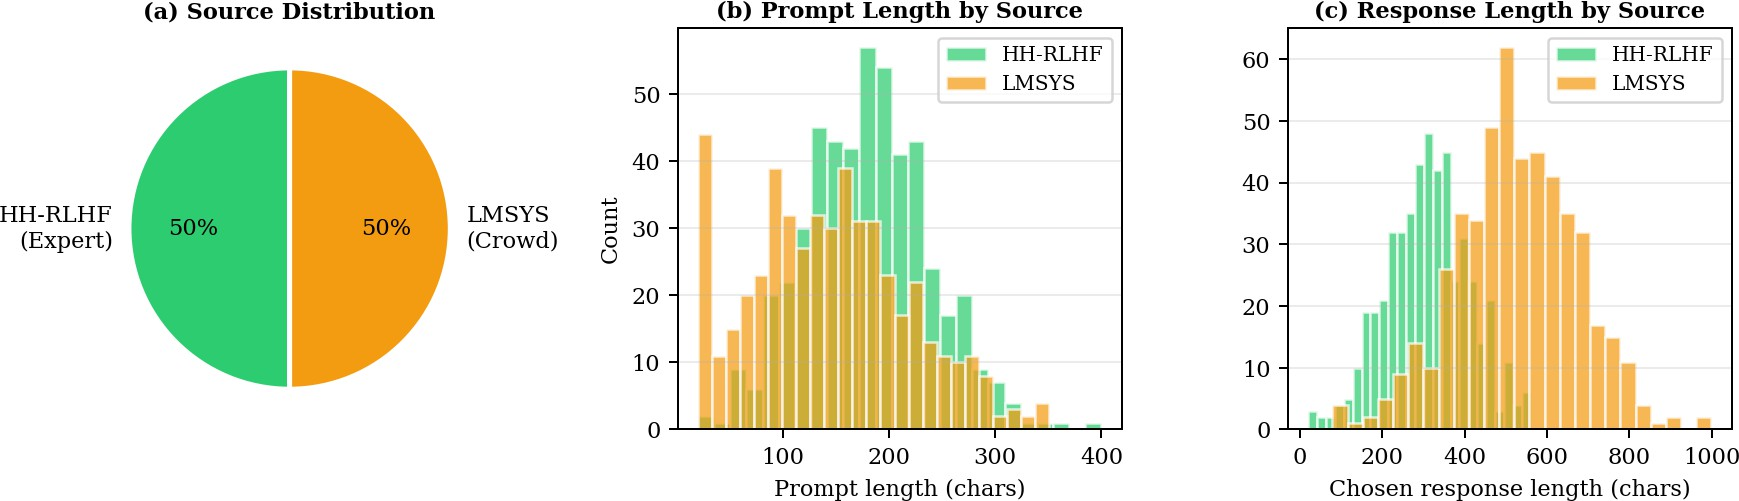
\includegraphics[width=\textwidth]{figures/rep_dataset.jpg}
\caption[Paper draft: dataset composition]{\reportedtag\ Reported in paper draft: combined dataset composition.}
\label{fig:rep-dataset}
\end{figure}

\begin{figure}[H]
\centering
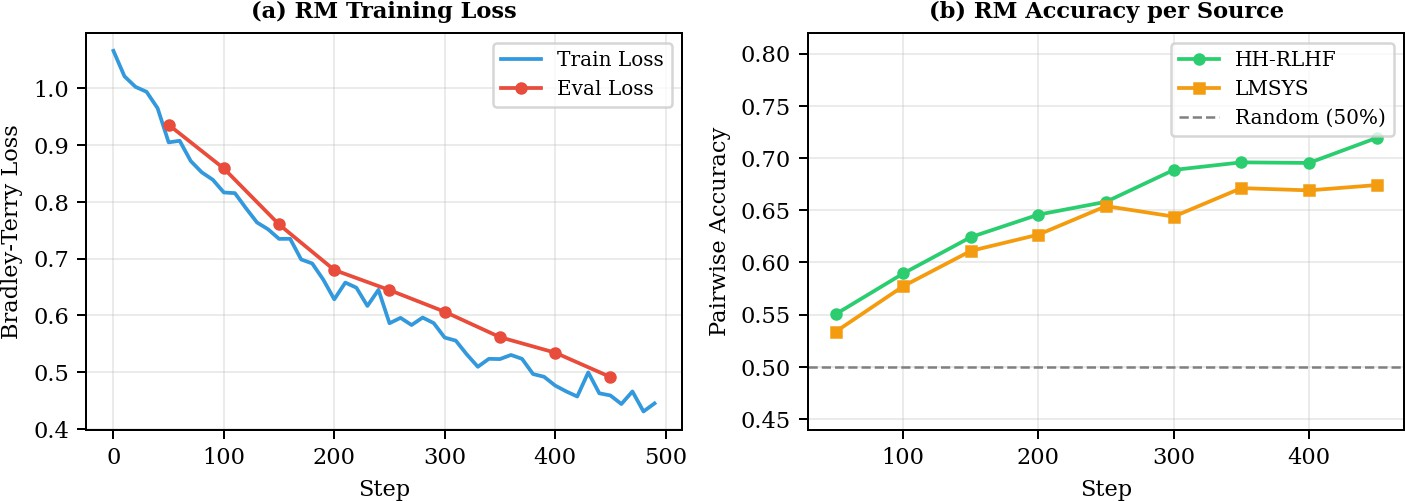
\includegraphics[width=0.92\textwidth]{figures/rep_rm_training.jpg}
\caption[Paper draft: reward-model training curves]{\reportedtag\ Reported in paper draft: (a) RM training loss, (b) RM accuracy per source.}
\label{fig:rep-rmtrain}
\end{figure}

\begin{figure}[H]
\centering
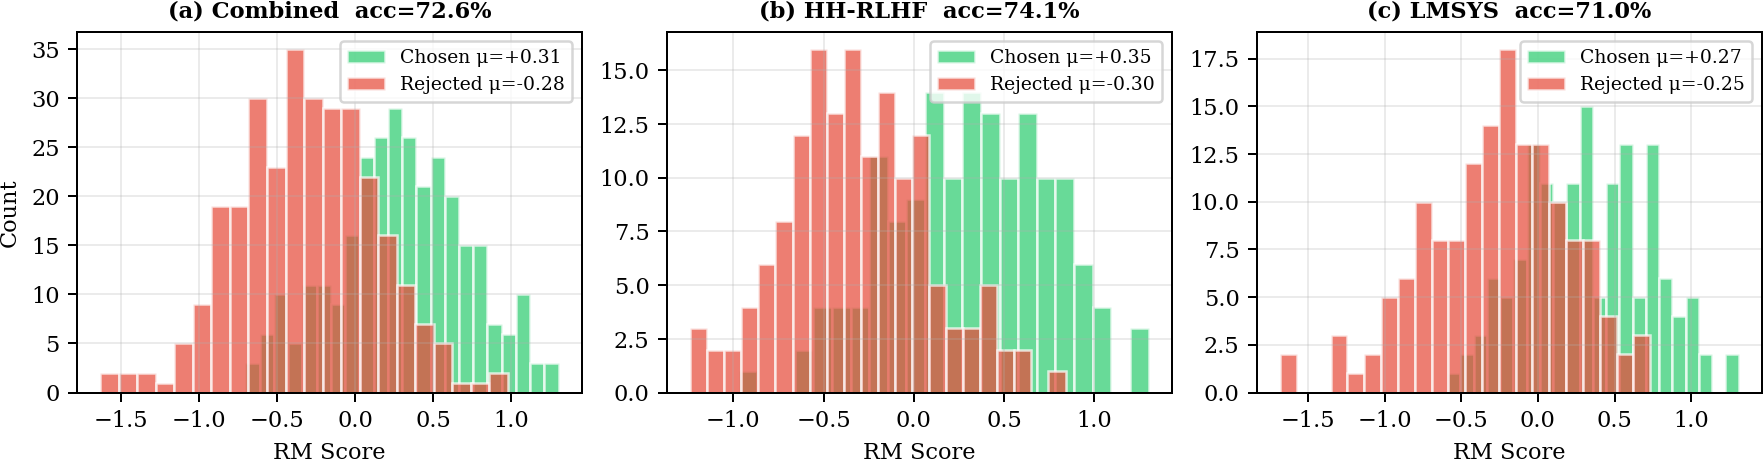
\includegraphics[width=\textwidth]{figures/rep_rm_scores.png}
\caption[Paper draft: reward-model score distributions]{\reportedtag\ Reported in paper draft: RM score distributions for chosen vs.\ rejected responses.}
\label{fig:rep-rmscores}
\end{figure}

\begin{figure}[H]
\centering
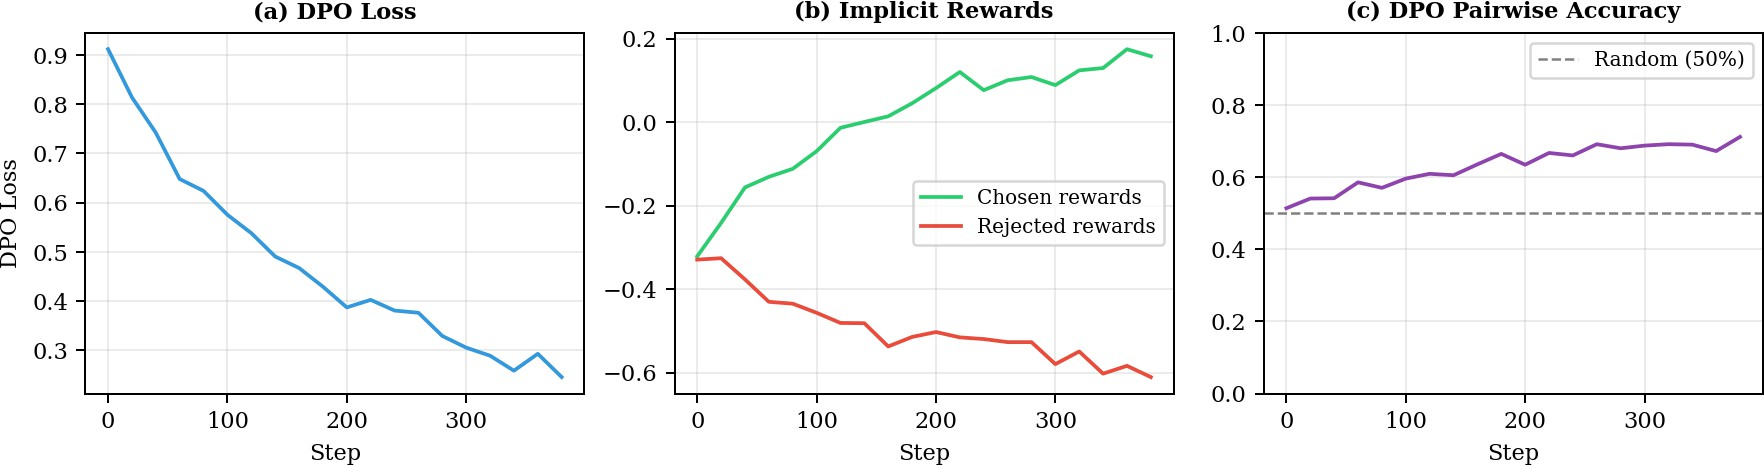
\includegraphics[width=\textwidth]{figures/rep_dpo_curves.jpg}
\caption[Paper draft: DPO training curves]{\reportedtag\ Reported in paper draft: DPO loss, implicit rewards and pairwise accuracy.}
\label{fig:rep-dpocurves}
\end{figure}

\begin{figure}[H]
\centering
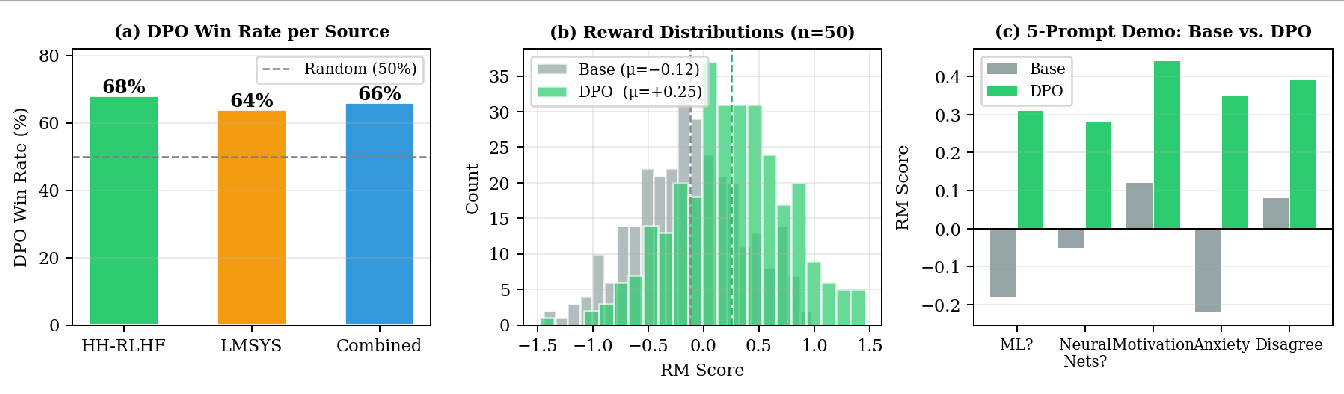
\includegraphics[width=\textwidth]{figures/rep_dpo_eval.png}
\caption[Paper draft: DPO evaluation summary]{\reportedtag\ Reported in paper draft: DPO win rates, reward distributions and demo-reel scores.}
\label{fig:rep-dpoeval}
\end{figure}

\subsection{Reported vs.\ measured}
Table~\ref{tab:rep-vs-meas} places the headline numbers side by side.

\begin{table}[!htbp]
\centering
\caption[Paper draft vs.\ measured results]{Headline metrics: paper draft (reported\reportedtag) vs.\ submitted notebooks (measured).}
\label{tab:rep-vs-meas}
\small
\begin{tabular}{@{}lccc@{}}
\toprule
\textbf{Metric} & \textbf{Reported\reportedtag} & \textbf{Measured A} & \textbf{Measured B}\\
\midrule
RM accuracy, combined & 72.6\% & 59.2\% & 59.6\%\\
RM accuracy, HH-RLHF & 74.1\% & 59.2\% & 57.9\%\\
RM accuracy, LMSYS & 71.0\% & 59.2\% & 64.8\%\\
RM per-source gap & 3.1 pp & 0.0 pp & 6.9 pp\\
DPO win rate, combined & 66\% & 50\% & 50\%\\
DPO win rate, HH-RLHF / LMSYS & 68\% / 64\% & 56\% / 44\% & 24\% / 76\%\\
Demo-reel DPO wins & 5/5 & 3/5 & 2/5\\
Demo-reel mean $\Delta$ & $+0.40$ & $+0.124$ & $-0.003$\\
\bottomrule
\end{tabular}
\end{table}

The draft's general claims hold up in the measured data: the reward model beats chance and is balanced across sources under the 10-point rule, and DPO trains stably while updating few parameters. Its numbers do not hold up. Measured reward-model accuracy is about 13 points lower, and the measured win rate shows no overall gain over the base model. The draft's ablation table (Table~\ref{tab:rep-ablation}) was never re-run, so its single-source rows have nothing measured to compare with.

\section{Discussion}
\label{sec:discussion}

\subsection{Why is reward-model accuracy around 59\%?}
Several factors limit the reward model:
\begin{itemize}
  \item \textbf{Noisy labels.} Many HH-RLHF pairs are almost identical, and the Llama~2 authors found their reward models were close to guessing on pairs that annotators had marked as only slightly different~\cite{touvron2023llama2}. LMSYS votes come from anonymous visitors with no guidelines. On such data even a perfect model could not reach anywhere near 100\%.
  \item \textbf{Small model, little data.} Reward-model accuracy improves with model size and with data~\cite{bai2022hh,gao2023overoptimization}. Ours has 184M parameters, LoRA trains only 1--2\% of them, and it sees between 3,500 and 7,000 pairs.
  \item \textbf{Truncation.} Inputs are cut to 512 tokens, so for long multi-turn prompts the decisive part of a response may be truncated away.
\end{itemize}
The near-identical accuracy of A and B suggests that, of these, data quantity is not the binding constraint at this scale.

\subsection{Why does successful DPO training not yield a higher win rate?}
DPO reached 80--95\% implicit-reward accuracy, yet the policy is not preferred by the reward model overall. Three mechanisms explain this.

\paragraph{1. The training answers were written by other models.} Every chosen and rejected answer in both datasets came from some \emph{other} model: Anthropic's models for HH-RLHF, and dozens of public chatbots, many far bigger than TinyLlama, for LMSYS. DPO can make such answers \emph{relatively} more or less likely, but it cannot make a 1.1B model write like GPT-4. Configuration B shows the usual sign of this: the probability of both the chosen and the rejected answer goes down (Table~\ref{tab:dpo-log}). The model mostly learns what \emph{not} to say on those specific pairs, which carries over only partly to the answers it writes itself.

\paragraph{2. A weak judge hides real effects.} Suppose the aligned model really is better on a share $p$ of prompts, and the judge agrees with the true preference with probability $a$. The win rate we \emph{observe} is then
\begin{equation}
  \mathrm{WR}_{\text{obs}} = a\,p + (1-a)(1-p).
\end{equation}
Our judge's measured accuracy is about $a\approx0.59$. Even if the draft's figure of $p=0.66$ were the true win rate, we would observe only about $0.59\times0.66 + 0.41\times0.34\approx0.53$, which 50 prompts cannot tell apart from 50\%. So our measured 50\% fits a small real improvement just as well as no improvement. Only a stronger, independent judge can settle it.

\paragraph{3. The judge and the trained model share blind spots.} The reward model that measures the gain has the same weaknesses that preference training can exploit, as the ``2 + 3'' answer showed. Some of the gains it reports may be reward hacking, and some of the losses may be the judge's own noise.

\subsection{What the per-source breakdown revealed}
The main point of the project is that looking at each source separately shows things that one overall number hides, and configuration B demonstrates it best. Its overall win rate of 50\% would usually be reported as ``DPO had no effect'', yet split by source the effect is large and goes in opposite directions (24\% against 76\%). We can suggest possible reasons, but these are guesses we have not tested: (i) the HH-heavy DPO data and larger LoRA let the model fit the HH-RLHF training pairs most closely, and the strong downward drift of the implicit rewards points to over-fitting that hurts its answers to similar prompts; (ii) configuration B's reward model is itself more accurate on LMSYS (64.8\%) than on HH-RLHF (57.9\%), so its verdicts on LMSYS prompts deserve more trust; (iii) longer, more structured answers, typical of LMSYS chosen answers, may score well on open Arena questions but badly as replies inside short HH dialogues. Without the per-source split we would have seen none of this.

\subsection{Comparison of the two configurations}
\begin{table}[!htbp]
\centering
\caption[Configuration A vs.\ B]{Summary comparison of the two measured configurations.}
\label{tab:ab-compare}
\small
\begin{tabularx}{\textwidth}{@{}L{5.6cm}YY@{}}
\toprule
\textbf{Aspect} & \textbf{A (balanced, light DPO)} & \textbf{B (HH-weighted, heavy DPO)}\\
\midrule
RM accuracy (combined / per-source gap) & 59.2\% / 0.0 pp & 59.6\% / 6.9 pp\\
RM mean reward gap & 0.069 & 0.118\\
Final DPO loss / implicit accuracy & $\approx$0.54 / $\approx$80\% & $\approx$0.21 / $\approx$95\%\\
Held-out win rate (combined) & 50\% & 50\%\\
Held-out win rate spread across sources & 12 pp (not significant) & 52 pp (significant)\\
Demo-reel mean $\Delta$ & $+0.124$ & $-0.003$\\
Trainable policy parameters & $\approx$4.5M & $\approx$25.2M\\
Interpretation & Mild, balanced, statistically null effect & Strong source-dependent shift; signs of over-fitting\\
\bottomrule
\end{tabularx}
\end{table}

Configuration A is the cautious, well-behaved run. Configuration B shows that a stronger DPO update with more trainable parameters can change the model a lot, but in different directions for different kinds of prompt. More aggressive preference training is not automatically better, and the evaluation has to be able to show where the change goes.

\subsection{Validity of the evaluation}
Three things limit how much these results can tell us. First, each prompt gets one sampled answer per model, so chance plays a large part; several samples per prompt would help. Second, the reward model is a weak stand-in for human judgement and can be gamed. Third, 25 prompts per source can only reveal large effects. None of this makes the measured numbers wrong, but it limits the conclusions we can draw, and it shapes the future work in Chapter~\ref{ch:conclusion}.

\section{Summary}
Both Kaggle reward models score about 59\%, above chance, and are balanced across sources under our 10-point rule; the smaller laptop run reaches 57\%. DPO training goes smoothly in every configuration, but the aligned models are not preferred over the base model overall in the Kaggle runs (50\% win rate), and configuration B shows a strong split by source that the overall figure hides. The laptop run's 57\% win rate on 30 prompts is not significant. The ``2 + 3'' example shows how a small reward model can be fooled. The higher numbers from our earlier paper draft are shown separately and are not reproduced by our code.

\chapter{Conclusion and Future Scope}
\label{ch:conclusion}

Our goal was a preference-alignment pipeline that runs on free hardware, with every result measured separately for each data source. Here we hold the work up against the objectives from Chapter~\ref{ch:intro}, state what we conclude and where the work falls short, propose next steps, and note what the project taught us.

\section{What Was Done}
\label{sec:summary}

We built and ran a pipeline that goes all the way from raw preference data to reward modelling and Direct Preference Optimization. It draws on two public datasets with very different backgrounds: HH-RLHF, labelled by paid annotators working from written guidelines, and LMSYS Chatbot Arena, voted on by the general public. Both were put into one format, filtered by the same rules, balanced, and split so that every split holds both sources. On Kaggle's free T4 GPUs we trained a DeBERTa-v3-base reward model, with LoRA and a saved pooler, on the Bradley--Terry loss, and aligned a 4-bit TinyLlama-1.1B-Chat with DPO using LoRA, a paged 8-bit optimiser and gradient checkpointing. We repeated this for two data mixes and broke every result down by source. Finally, the notebook became a reusable system, a command-line pipeline and a web application, and a smaller version was trained from scratch on an 8\,GB Apple M1 laptop.

\section{Objectives Met}
\label{sec:achievements}

\begin{table}[!htbp]
\centering
\caption[Status of objectives]{Status of the objectives listed in Section~\ref{sec:objectives}.}
\label{tab:objectives}
\small
\begin{tabularx}{\textwidth}{@{}L{0.8cm}YL{1.9cm}Y@{}}
\toprule
\textbf{Obj.} & \textbf{Objective} & \textbf{Status} & \textbf{Evidence}\\
\midrule
O1 & One tagged, per-source split dataset & Met & 40.5K HH-RLHF and 36.5K LMSYS clean pairs; Tables~\ref{tab:datastats}, \ref{tab:splits}\\
O2 & DeBERTa-v3 reward model with LoRA & Met & Three trained reward models (A, B, local)\\
O3 & Per-source reward-model accuracy with 10-point rule & Met & 59.2\%, 59.6\%, 57.1\%; gaps 0.0, 6.9 and 9.5 points\\
O4 & DPO-align TinyLlama on one T4 & Met & 1.14\,GB policy footprint; 80--95\% implicit accuracy\\
O5 & Base vs.\ DPO per source & Met (no clear gain) & 50\% overall in A and B; 24\%/76\% split in B\\
O6 & Reusable system with web application & Met & \texttt{run\_pipeline.py}, \texttt{app.py}; Figures~\ref{fig:ui-top}--\ref{fig:ui-about}\\
O7 & Honest critical analysis & Met & Section~\ref{sec:discussion}; reward-hacking example\\
\bottomrule
\end{tabularx}
\end{table}

\section{Conclusions}
\label{sec:conclusions}

\begin{enumerate}
  \item \textbf{Expert and crowd preferences can share one training set.} With our conversion and filtering neither dataset drowns out the other. All three reward models rank unseen pairs better than chance and pass the 10-point balance rule, and the balanced configuration scores exactly the same on both sources.
  \item \textbf{At this size, the reward model is the bottleneck.} A 184M-parameter encoder with LoRA sits at about 57--60\% accuracy in all three runs, whether it was trained on 1,750, 3,500 or 7,000 pairs. That holds it back both as a training signal and as a judge.
  \item \textbf{Good DPO training curves are not proof of alignment.} 80--95\% implicit-reward accuracy went hand in hand with a 50\% win rate on new prompts. The training curves measure how well the model fits the stored pairs, not whether the answers it writes got better.
  \item \textbf{Split the results by source.} In configuration B, an overall win rate of exactly 50\% concealed a significant 24\% versus 76\% split between the two sources. From the total alone we would have concluded, wrongly, that DPO changed nothing.
  \item \textbf{A small judge is easy to fool.} The single biggest score gain in the whole study, on the ``2 + 3'' prompt, went to a wrong answer. Any claim of better alignment needs a judge that had no part in training.
  \item \textbf{The system can be reproduced on ordinary hardware.} The packaged pipeline retrained everything on an 8\,GB laptop in about an hour and a half, produced exactly the same data counts as the notebook, and serves the trained models through a web app.
  \item \textbf{Report what was actually measured.} The higher figures in our earlier paper draft could not be reproduced, so the measured results are the main findings and the draft figures are clearly labelled. Having saved, re-runnable code is what let us make this check.
\end{enumerate}

\section{Limitations}
\label{sec:limitations}

\begin{itemize}
  \item \textbf{The reward model is also the judge.} The aligned model is graded by the same kind of reward model it was trained to please. That judge is weak (around 59\%), gameable and not independent, and we used neither human raters nor an outside model.
  \item \textbf{Small samples.} With 15--25 prompts per source and one answer per model, only big effects show up, and chance has a lot of say.
  \item \textbf{Small models.} What holds for a 184M reward model and a 1.1B policy may not hold for models of 7B and up.
  \item \textbf{No supervised fine-tuning on our data.} DPO is applied directly to a chat model, using answers that other, often far larger, models wrote.
  \item \textbf{Length limits.} Text fields are capped at 1,500 characters and inputs at 512 tokens (256 for DPO on the laptop), which may cut away exactly the part of an answer that decided the vote. We did not run a length-controlled evaluation.
  \item \textbf{Helpfulness only.} Harmlessness, honesty and factual accuracy were not measured, and the reward-hacking case shows that accuracy can actually get worse.
  \item \textbf{Few ablations.} We ran only two Kaggle mixes, changed several settings between them, and never trained single-source reward models to compare against.
  \item \textbf{The draft's numbers.} The figures in the earlier paper draft are not backed by the code we are submitting.
\end{itemize}

\section{Future Scope}
\label{sec:future}

\subsection{Better evaluation}
\begin{itemize}
  \item Have a strong outside model (GPT-4-class or a large open model) judge base and DPO answers, swapping their order to cancel the position bias reported by Zheng \emph{et al.}~\cite{zheng2023judging}, and run a small blind rating study with fellow students.
  \item Report standard benchmarks such as MT-Bench, length-controlled AlpacaEval and RewardBench~\cite{lambert2024rewardbench} so that our numbers can be set beside published ones.
  \item Evaluate on at least 200 prompts per source with several answers each, and always report confidence intervals and significance tests.
\end{itemize}

\subsection{Better reward models}
\begin{itemize}
  \item Move to DeBERTa-v3-large, or to a 1--2B decoder reward model trained with QLoRA, with longer inputs.
  \item Train single-source and mixed reward models under identical settings to measure directly what mixing buys.
  \item Give the reward model a separate output head for each source and learn how to combine them.
  \item Bring in a third source with yet another labelling style, such as UltraFeedback~\cite{cui2023ultrafeedback} or HelpSteer2~\cite{wang2024helpsteer2}, and drop pairs where annotators disagree.
\end{itemize}

\subsection{Better policy training}
\begin{itemize}
  \item Run supervised fine-tuning on the chosen answers before DPO. This completes the InstructGPT recipe and narrows the gap between the training answers and the model's own style.
  \item Build preference pairs from TinyLlama's \emph{own} answers, rank them with a strong judge, and run DPO again in several rounds.
  \item Compare DPO against IPO~\cite{azar2024ipo}, KTO~\cite{ethayarajh2024kto}, ORPO~\cite{hong2024orpo} and SimPO~\cite{meng2024simpo}; KTO could also make use of LMSYS rows that only have a clear winner or a clear loser.
  \item Pick $\beta$ and the number of epochs by the per-source win rate on a validation prompt set, not by DPO loss.
  \item Scale the policy up to 3--8B parameters, for example Llama-3-8B or Mistral-7B with QLoRA, on bigger GPUs.
\end{itemize}

\subsection{Safety and the application}
\begin{itemize}
  \item Add the HH-RLHF harmless-base split and test safety on its own, or add a Constitutional-AI-style self-check~\cite{bai2022cai} at generation time.
  \item Give the web app a third column with an independent judge's verdict beside the reward model's, so reward hacking can be caught live, and let users cast their own vote to gather new preference data.
\end{itemize}

\section{What We Learned}
\label{sec:learning}

\begin{itemize}
  \item How preference learning works in theory: the Bradley--Terry model, KL-limited reinforcement learning, and how DPO's loss falls out of the two.
  \item How to train big models on small hardware with LoRA, 4-bit NF4, paged 8-bit optimisers and gradient checkpointing, and what each costs in memory on CUDA and on Apple's MPS.
  \item How to work with data from mixed sources: designing a shared format, splitting without leakage, and seeing how a small filtering choice can silently reshape a dataset.
  \item How to track down failures that throw no error: 16-bit overflow, a randomly initialised layer that was never saved, models on the wrong GPU, and clashing library versions.
  \item How to turn research code into something usable: a package with clear stages, configuration presets, automatic hardware detection and a web interface.
  \item Why honesty in experiments matters: evaluating by group, knowing how little a small test set can say, spotting reward hacking, and reporting null or negative results as plainly as positive ones.
\end{itemize}

\section{Closing Remarks}
Preference alignment is often presented as a fixed recipe: train a reward model, run DPO, quote a win rate. Doing it ourselves at small scale showed that any step can go wrong without warning. Reward models plateau, DPO can fit its training pairs without improving what the model writes, and a single win rate can hide two opposite effects. By mixing datasets labelled in different ways and reporting every number per source, we turned those hidden failures into results we could see and measure. We regard this as the main contribution of our project, and we hope the pipeline and application we built give a useful starting point for the stronger judges, larger reward models and on-policy training described above.


\cleardoublepage
\addcontentsline{toc}{chapter}{References}
\bibliographystyle{ieeetr}
\bibliography{references}

\appendix
\chapter{Complete Source Code (Configuration A)}
\label{app:code}

This appendix reproduces every code cell of the executed notebook \texttt{mini-6\_}\allowbreak\texttt{working.ipynb} (configuration A) in order. Non-ASCII symbols used for console decoration in the original notebook (emoji, arrows) have been removed or replaced with ASCII equivalents; the code is otherwise unchanged. Markdown cells are omitted; their content is covered in Chapters~\ref{ch:method} and~\ref{ch:impl}.

\lstinputlisting[style=py, caption={Complete notebook source, configuration A (\texttt{mini-6\_working}).}, label={lst:fullA}, basicstyle=\ttfamily\scriptsize]{code/configA_full.py}

\chapter{Code Changes for Configuration B}
\label{app:codeB}

Configuration B (\texttt{mini-7-fixed.ipynb}) uses the same code as Appendix~\ref{app:code} except for the cells listed below: the stale-checkpoint cleaner (cell 0), the HH-weighted sampling (cell 13), the larger LoRA rank for the reward model (cell 18), the slower and longer reward-model schedule (cell 20), the 2:1 HH-weighted DPO data (cell 30), and the DPO configuration with MLP adapters, lower learning rate, higher $\beta$ and best-checkpoint reload (cell 31).

\lstinputlisting[style=py, caption={Changed cells, configuration B (\texttt{mini-7-fixed}).}, label={lst:fullB}, basicstyle=\ttfamily\scriptsize]{code/configB_changed.py}

\chapter{Sample Model Outputs}
\label{app:outputs}

The complete console output of the five-prompt demo reel for both configurations is reproduced below, exactly as printed by the notebooks (decorative symbols removed). Responses are cut at 200 new tokens, which is why some end mid-sentence. The reward scores are those of the configuration's own reward model; scores from different configurations are \emph{not} comparable, because each reward model has its own arbitrary offset.

\section{Configuration A}
\lstinputlisting[style=py, language={}, numbers=none, caption={Demo-reel output, configuration A.}, label={lst:outA}, basicstyle=\ttfamily\scriptsize, breaklines=true]{code/demo_outputs_A.txt}

\section{Configuration B}
\lstinputlisting[style=py, language={}, numbers=none, caption={Demo-reel output, configuration B.}, label={lst:outB}, basicstyle=\ttfamily\scriptsize, breaklines=true]{code/demo_outputs_B.txt}

\chapter{Reproduction Guide}
\label{app:repro}

\section{Requirements}
\begin{itemize}
  \item A Kaggle account with phone verification (required for GPU and internet access).
  \item The LMSYS Chatbot Arena \texttt{train.csv} attached as an input dataset (from the Kaggle competition \emph{LMSYS -- Chatbot Arena Human Preference Predictions}).
  \item Notebook settings: \emph{Accelerator: GPU T4 $\times$2}, \emph{Internet: On}.
\end{itemize}

\section{Steps}
\begin{enumerate}
  \item Upload the notebook (\texttt{mini-6\_working.ipynb} for configuration A or \texttt{mini-7-fixed.ipynb} for configuration B) to Kaggle and attach \texttt{train.csv}.
  \item Run the installation cell, then \emph{restart the kernel} once so that the upgraded \texttt{torchao} and \texttt{peft} are imported cleanly.
  \item Run all cells. The first run downloads HH-RLHF, DeBERTa-v3-base and TinyLlama, trains both models and takes about 2.5--3 hours.
  \item Use \emph{Save Version $\rightarrow$ Quick Save} so that \texttt{reward\_model/} and \texttt{finetuned\_llm/} are kept as notebook output.
  \item In later sessions, attach the saved notebook output as an input dataset. The path-resolution cell (Listing~\ref{lst:persist}) finds the adapters automatically and every training stage is skipped.
  \item Run the interactive cell on its own to compare models on new prompts; type \texttt{quit} to stop.
\end{enumerate}

\section{Output Artefacts}
\begin{table}[!htbp]
\centering
\caption[Files produced by a complete run]{Files produced by a complete run.}
\label{tab:artefacts}
\small
\begin{tabularx}{\textwidth}{@{}L{5.6cm}Y@{}}
\toprule
\textbf{Path (under \texttt{/kaggle/working})} & \textbf{Content}\\
\midrule
\texttt{reward\_model/} & LoRA adapter, pooler and classifier weights, tokenizer, \texttt{training\_log.json}\\
\texttt{finetuned\_llm/} & DPO LoRA adapter, tokenizer, \texttt{training\_log.json}\\
\texttt{plots/}\allowbreak\texttt{dataset\_composition.png} & Figure~\ref{fig:m6-dataset} / \ref{fig:m7-dataset}\\
\texttt{plots/}\allowbreak\texttt{rm\_validation\_per\_source.png} & Figure~\ref{fig:m6-rmdist} / \ref{fig:m7-rmdist}\\
\texttt{plots/}\allowbreak\texttt{rm\_loss\_curve.png} & Figure~\ref{fig:m6-rmloss} / \ref{fig:m7-rmloss}\\
\texttt{plots/}\allowbreak\texttt{dpo\_curves.png} & Figure~\ref{fig:m6-dpocurves} / \ref{fig:m7-dpocurves}\\
\texttt{plots/}\allowbreak\texttt{demo\_comparison.png} & Figure~\ref{fig:demo}\\
\texttt{plots/}\allowbreak\texttt{before\_after\_headline.png} & Figure~\ref{fig:m6-headline} / \ref{fig:m7-headline}\\
\texttt{demo\_results.csv} & Five-prompt demo reel responses and scores\\
\texttt{batch\_eval.csv} & 50-prompt held-out evaluation with source labels\\
\texttt{interactive\_session.csv} & Log of the interactive session\\
\bottomrule
\end{tabularx}
\end{table}

\section{Running the Packaged System}
The folder \texttt{rlhf\_system} contains the system described in Section~\ref{sec:system}.
\begin{enumerate}
  \item Create the environment once: \texttt{python3 -m venv .venv} and \texttt{.venv/bin/pip install -r requirements-app.txt} (add \texttt{requirements-train.txt} to train).
  \item Train on Kaggle: \texttt{python run\_pipeline.py -{}-config A} (or \texttt{B}). Train on an 8\,GB Mac: \texttt{PYTORCH\_MPS\_HIGH\_WATERMARK\_RATIO=0.0 python run\_pipeline.py -{}-config local}.
  \item Single stages: add \texttt{-{}-stage data}, \texttt{rm}, \texttt{dpo} or \texttt{eval}. Finished stages are skipped automatically.
  \item Start the web application with \texttt{python app.py} and open \url{http://127.0.0.1:7860}. Adapters placed in \texttt{models/} are used first; otherwise the newest pipeline output is loaded.
\end{enumerate}


\end{document}
